% Options for packages loaded elsewhere
\PassOptionsToPackage{unicode}{hyperref}
\PassOptionsToPackage{hyphens}{url}
\documentclass[
]{article}
\usepackage{xcolor}
\usepackage{amsmath,amssymb}
\setcounter{secnumdepth}{-\maxdimen} % remove section numbering
\usepackage{iftex}
\ifPDFTeX
  \usepackage[T1]{fontenc}
  \usepackage[utf8]{inputenc}
  \usepackage{textcomp} % provide euro and other symbols
\else % if luatex or xetex
  \usepackage{unicode-math} % this also loads fontspec
  \defaultfontfeatures{Scale=MatchLowercase}
  \defaultfontfeatures[\rmfamily]{Ligatures=TeX,Scale=1}
\fi
\usepackage{lmodern}
\ifPDFTeX\else
  % xetex/luatex font selection
\fi
% Use upquote if available, for straight quotes in verbatim environments
\IfFileExists{upquote.sty}{\usepackage{upquote}}{}
\IfFileExists{microtype.sty}{% use microtype if available
  \usepackage[]{microtype}
  \UseMicrotypeSet[protrusion]{basicmath} % disable protrusion for tt fonts
}{}
\makeatletter
\@ifundefined{KOMAClassName}{% if non-KOMA class
  \IfFileExists{parskip.sty}{%
    \usepackage{parskip}
  }{% else
    \setlength{\parindent}{0pt}
    \setlength{\parskip}{6pt plus 2pt minus 1pt}}
}{% if KOMA class
  \KOMAoptions{parskip=half}}
\makeatother
\usepackage{graphicx}
\makeatletter
\newsavebox\pandoc@box
\newcommand*\pandocbounded[1]{% scales image to fit in text height/width
  \sbox\pandoc@box{#1}%
  \Gscale@div\@tempa{\textheight}{\dimexpr\ht\pandoc@box+\dp\pandoc@box\relax}%
  \Gscale@div\@tempb{\linewidth}{\wd\pandoc@box}%
  \ifdim\@tempb\p@<\@tempa\p@\let\@tempa\@tempb\fi% select the smaller of both
  \ifdim\@tempa\p@<\p@\scalebox{\@tempa}{\usebox\pandoc@box}%
  \else\usebox{\pandoc@box}%
  \fi%
}
% Set default figure placement to htbp
\def\fps@figure{htbp}
\makeatother
\setlength{\emergencystretch}{3em} % prevent overfull lines
\providecommand{\tightlist}{%
  \setlength{\itemsep}{0pt}\setlength{\parskip}{0pt}}
\usepackage{bookmark}
\IfFileExists{xurl.sty}{\usepackage{xurl}}{} % add URL line breaks if available
\urlstyle{same}
\hypersetup{
  hidelinks,
  pdfcreator={LaTeX via pandoc}}

\author{}
\date{}

\begin{document}

Paul Koop


\includegraphics[width=4.92849in,height=4.92031in]{media/image6.png}

Die letzte Freiheit

Eine Geschichte zum Posthumanismus

Eine Fortsetzung von I.R.A.R.A.H antwortet

Die Geschichte spielt in einer nahen Zukunft, in der Europa durch die
Machtübernahme von InSim in hochgradig kontrollierte "Autonome Cities"
aufgeteilt ist. Diese Stadtstaaten sind technologisch fortschrittlich,
aber ihre Gesellschaften sind postdemokratisch organisiert, was
bedeutet, dass Algorithmen und KI die Entscheidungen treffen, die zuvor
in die Hände der Bürger gehörten. Überwachung ist allgegenwärtig, und
die soziale Kontrolle basiert auf Sozialkreditsystemen und
technokratischen Strukturen.

Anna Jensen und Leonard Eriksson, zwei junge Wissenschaftler, arbeiten
im Bereich der Quantenverschlüsselung im gesicherten Quantencomputing
ETZ (Encryption and Telecommunication Zone). Sie beginnen, an den Regeln
und der Kontrolle der Autonomen Cities zu zweifeln, als sie entdecken,
dass InSim bestimmte Technologien und historische Informationen
manipuliert, um die Bevölkerung im Unklaren über die Vergangenheit und
die wahre Machtverteilung zu lassen.

Inhaltsverzeichnis

\hyperref[annas-leben-in-der-encryption-and-telecommunication-zone]{\textbf{Annas
Leben in der Encryption and Telecommunication Zone 2}}

\hyperref[anna-lernt-leonard-kennen]{\textbf{Anna lernt Leonard kennen
8}}

\hyperref[die-entdeckung-von-ars]{\textbf{Die Entdeckung von ARS 19}}

\hyperref[geschichtsforschung-mit-ars]{\textbf{Geschichtsforschung mit
ARS 37}}

\hyperref[die-ausreise]{\textbf{Die Ausreise 40}}

\hyperref[ein-neues-leben]{\textbf{Ein neues Leben 52}}

\hyperref[epilog]{\textbf{Epilog 58}}

\hyperref[einfluxfcsse-und-inspirationen-fuxfcr-das-pompeji-projekt-i.r.a.r.a.h]{\textbf{Einflüsse
und Inspirationen für Das Pompeji-Projekt I.R.A.R.A.H 65}}

\section{Annas Leben in der Encryption and Telecommunication
Zone}\label{annas-leben-in-der-encryption-and-telecommunication-zone}

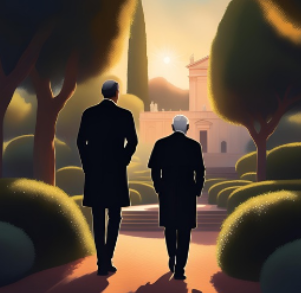
\includegraphics[width=2.64583in,height=2.59375in]{media/image1.png}

Die Lichtstreifen der Überwachungskameras huschten über die kargen
Betonwände des Quantencomputing ETZ, während Anna Jensen mit gesenktem
Kopf durch die Sicherheitsschleuse trat. Das Summen der Scanner und das
metallische Klicken der Zugangskarten waren ein ständiger Teil ihres
Morgens. Sie wusste, dass jede Bewegung registriert wurde, jedes Muster
ihres täglichen Weges durch die sterile Korridore der verschachtelten
Büroanlagen des ETZ aufgezeichnet war -- eine Routine, die ihr längst
zur Gewohnheit geworden war und doch wie ein unsichtbares Netz um sie
lag.

Ihr Arbeitsplatz war eine Glaskabine, die sich inmitten der
labyrinthartigen Anlage befand, abgeschottet und doch durchsichtiger als
ihr lieb war. Auf dem Schreibtisch leuchteten die Bildschirme mit einer
Kaskade von Datenströmen, die in grün blauem Flimmern über die Anzeige
jagten. Anna setzte sich, nahm die Kopfhörer ab, die sie gegen die
monotone Geräuschkulisse der Serverräume abgeschirmt hatten, und schob
eine lose Haarsträhne hinters Ohr. Für einen Moment verharrte sie,
starrte auf die Zahlenreihen vor sich, die sich beständig veränderten,
als versuchten sie, ihrem Blick zu entkommen.

Ihre Aufgabe bestand darin, Algorithmen zu optimieren, die
verschlüsselte Kommunikationskanäle überwachten und Anomalien in den
Datenströmen erkannten. Mit einem Tastendruck öffnete sie das Protokoll
des Nachtdienstes. Verdächtige Abweichungen: zwei. Es war Routinearbeit,
die Datenpakete zu analysieren, nach Mustern zu suchen, die auf
Unregelmäßigkeiten oder mögliche Verstöße hinwiesen. Doch je mehr Anna
sich in die verschlüsselten Netzwerke vertiefte, desto stärker drängte
sich ihr der Gedanke auf, dass sie in Wirklichkeit keinen Schutz für die
Menschen, sondern nur das perfekte Überwachungsinstrument erschuf.

Sie blinzelte und lehnte sich zurück, die Hände ruhten auf der Tastatur.
Für einen Moment ließ sie den Blick über den Raum schweifen, als könnte
sie dort eine Antwort finden. Aber alles, was sie sah, waren ihre
eigenen Spiegelbilder in den Glaswänden und die gesichtslosen
Silhouetten der anderen Mitarbeiter, die in ihren Kabinen über ihren
Bildschirmen hingen. Die Luft war erfüllt vom gleichmäßigen Brummen der
Server, eine Mischung aus mechanischer Präzision und menschlicher
Gleichgültigkeit, die sich wie ein Schleier über den Raum legte.

An diesem Morgen spürte Anna die Unruhe deutlicher als sonst -- ein
leises, nagendes Gefühl im Bauch, das sich nicht abschütteln ließ. Die
Vorstellung, dass jeder verschlüsselte Datenstrom, den sie prüfte, ein
Leben war, das sich unbemerkt durch die Ritzen des Systems schlängeln
wollte, ließ sie nicht los. Mit einem leichten Kopfschütteln rief sie
sich selbst zur Ordnung, beugte sich wieder über die Tastatur und begann
zu tippen. Doch in ihrem Hinterkopf nagte ein Gedanke, der sich nicht so
einfach wegdrücken ließ: Bin ich hier, um Menschen zu schützen -- oder
nur, um ihre Freiheit weiter einzuschränken?

Anna war sich nicht sicher, wann genau sie begonnen hatte, die ersten
Zweifel zu hegen. Vielleicht war es das letzte Update gewesen, bei dem
die Anweisungen plötzlich strenger, die Protokolle detaillierter
geworden waren. Vielleicht auch der Gedanke, dass ihre Arbeit nicht mehr
nur einem abstrakten Zweck diente, sondern in die intime Sphäre jeder
Kommunikation eindrang, jede Nachricht auf Zeichen des Abweichens
abklopfte. Oder war es etwas Tieferes, das sich in ihr regte, eine
Sehnsucht nach einer Welt, die nicht durch die kalte Logik der
Algorithmen beherrscht wurde?

Die Bildschirme vor ihr flackerten weiter, doch Anna konnte den Gedanken
nicht abschütteln, dass sie Teil eines riesigen Apparates war, der nicht
dem Wohl der Menschen diente, sondern sie in unsichtbare Ketten legte.

Anna atmete tief ein, als sie den Bildschirmen erneut ihre
Aufmerksamkeit schenkte. Die grünen und blauen Datenströme wogen sich
hypnotisch, doch sie blieben für sie nicht mehr nur eine Ansammlung von
Zahlen und Buchstaben. Stattdessen wurden sie zu einem Symbol der
Kontrolle, die über das Leben der Bürger schwebte. Jedes Paket, das sie
analysierte, war ein weiterer Baustein im kollektiven Gefängnis, in dem
die Menschen gefangen waren.

Inmitten ihrer Überlegungen fiel ihr Blick auf die schmale, digitale Uhr
an der Wand. Der Morgen verging, und mit jedem verstrichenen Moment
wuchs die Routine, die wie eine unsichtbare Hand um ihren Hals griff.
Sie wusste, dass sie bald an einer Besprechung teilnehmen sollte, die
sich mit den neuesten Sicherheitsprotokollen und den zu
implementierenden Algorithmus Updates befassen würde. Der Gedanke daran
ließ sie frösteln.

„Anna, alles in Ordnung?{\kern0pt}`` Die Stimme von Markus, einem
Kollegen, riss sie aus ihren Gedanken. Er stand an der Tür ihrer Kabine,
sein Gesicht war hinter dem Glas leicht verzerrt, aber sie konnte die
Besorgnis in seinen Augen erkennen.

„Ja, ich\ldots{} nur etwas nachdenklich``, antwortete sie und versuchte,
ein Lächeln aufzusetzen, das nicht ganz gelang. Markus nickte
verständnisvoll, doch sie wusste, dass er ihre Unruhe spürte.

„Kommst du zur Besprechung? Ich glaube, sie wollen uns die neuesten
Überwachungsprotokolle vorstellen``, sagte er und trat einen Schritt
näher. Seine Augen blitzten im gedämpften Licht der Kabine.

„Natürlich, ich komme gleich``, murmelte Anna und stellte fest, wie ihr
Magen sich zusammenzog. Die Gedanken an die unethischen Praktiken, die
sie täglich unterstützen musste, drängten sich in den Vordergrund. Das
Gespräch mit Markus war schnell beendet, und als er sich wieder
zurückzog, ließ er sie allein mit ihren Ängsten.

Die Minuten vergingen, und als die Zeit für die Besprechung näher
rückte, fühlte sie sich wie ein Soldat, der auf den Befehl zur Schlacht
wartete. Der Raum, der vorher so vertraut und sicher gewirkt hatte,
fühlte sich jetzt wie ein Käfig an. Sie stand auf und schloss den
Laptop, als der Alarm der Zeitansage durch den Raum hallte.

Die Versammlung fand in einem großen, anonymen Raum statt, dessen Wände
mit Bildschirmen gefüllt waren, die ständig wechselnde Datenströme
zeigten. Die Luft war elektrisch geladen, ein Gefühl, das sie nicht ganz
zuordnen konnte. Anna setzte sich an einen der Tische, umgeben von ihren
Kollegen, deren Gesichter ausdruckslos blieben. Das Licht flackerte und
tauchte den Raum in ein gespenstisches Licht, als der Leiter der
Besprechung, Herr Keller, ein älterer Mann mit einer Vorliebe für
strenge Anzüge, den Raum betrat.

„Willkommen zur heutigen Sitzung``, begann er mit einer Stimme, die so
kalt war wie die Technik, die sie bedienten. „Wir stehen vor neuen
Herausforderungen, und es ist unerlässlich, dass wir unsere
Überwachungsmechanismen weiter optimieren, um die Stabilität der
Autonomen Cities zu gewährleisten.``

Seine Worte hallten in Anna wider wie ein Echo der Unterdrückung. Sie
spürte, wie die Enttäuschung und Wut in ihr aufstiegen, während Herr
Keller über die Notwendigkeit sprach, alle potenziellen Bedrohungen für
das System zu eliminieren. Jedes Wort war ein weiterer Schlag ins
Gesicht der Freiheit, und sie wusste, dass es Zeit war, die Augen zu
öffnen und zu handeln.

Während er die neuesten Algorithmus Updates vorstellte, dachte Anna an
die Menschen außerhalb dieser Wände, die unter der Last der Kontrolle
litten. Sie sah die Gesichter der Menschen vor ihrem inneren Auge --
Familien, die sich nicht mehr frei bewegen konnten, Freunde, die nicht
mehr offen miteinander sprechen durften. Das Bild drängte sich auf, und
mit einem Mal wurde ihr klar, dass sie nicht länger schweigen konnte.

Sie fühlte sich wie ein Fremder in ihrem eigenen Leben, und als die
Sitzung endete und die Kollegen in ihre Kabinen zurückkehrten, spürte
Anna, dass eine Entscheidung fällig war. Entschlossen sammelte sie ihre
Sachen, ihre Gedanken in einem Sturm.

„Ich kann nicht mehr``, murmelte sie leise zu sich selbst. Es war an der
Zeit, das Spiel zu ändern, Zeit, ihre Zweifel in Taten zu verwandeln.
Sie wollte nicht länger Teil eines Systems sein, das die Freiheit der
Menschen erstickte.

Mit einem tiefen Atemzug verließ sie das Meeting und machte sich auf den
Weg zu Leonard, in der Hoffnung, dass auch er die gleiche Sehnsucht nach
Veränderung verspürte. Sie mussten gemeinsam herausfinden, wie sie die
Fesseln der Überwachung sprengen konnten, um die Wahrheit ans Licht zu
bringen.

Er war ein neuer Zuwachs im ETZ, doch sein Wissen und seine Fähigkeiten
im Quantencomputing waren beeindruckend. Leonard hatte sich in den
kurzen Wochen, in denen er im Team war, schnell einen Namen gemacht.
Seine analytischen Fähigkeiten waren unbestritten, doch es war nicht nur
seine Intelligenz, die Anna anzog. Es war die subtile Art, wie er
gelegentlich über die strengen Vorgaben des Systems sprach, als würde er
hinter der Fassade der Kontrolle nach einer Wahrheit suchen, die nur er
zu erkennen schien.

Sie erinnerte sich an die Gespräche, die sie gelegentlich in der
Kaffeeküche hatten. Bei einem dieser Treffen hatte Leonard leise, fast
verschwörerisch, gesagt: „Manchmal frage ich mich, ob wir wirklich die
Welt verbessern oder sie nur weiter einschränken.`` In diesem Moment
hatte Anna innegehalten, überrascht von der Direktheit seiner Worte.
Hatte er in den ersten Tagen, in denen sie sich kannten, bereits einen
Teil seiner Gedanken preisgegeben, oder war das nur ein flüchtiger
Moment, der nicht weiter verfolgt worden war?

Doch Leonard war auch vorsichtig. Er sprach nie laut über seine
Ansichten und wählte seine Worte mit Bedacht. Vielleicht war es die
Angst, belauscht zu werden, die ihn zurückhielt, oder die Befürchtung,
dass seine offenen Gedanken ihm in diesem starren System zum Verhängnis
werden könnten. Anna wusste, dass sie in einem Spiel lebten, in dem jede
unbedachte Äußerung möglicherweise das Ende ihrer Karriere bedeuten
konnte. Dennoch spürte sie eine tiefe Verbindung zu ihm, die über ihre
gemeinsamen Bedenken hinausging.

Ihr Blick wanderte zurück zu ihrem Monitor, aber sie konnte die Gedanken
an Leonard nicht loslassen. Was wäre, wenn sie ihm ihre eigenen Zweifel
anvertraute? Könnte sie ihm vertrauen? Der Gedanke, sich jemandem zu
öffnen, der ebenfalls in dieser geknechteten Welt nach Freiheit strebte,
war sowohl verlockend als auch beängstigend. Anna spürte ein Ziehen in
ihrem Bauch -- eine Mischung aus Hoffnung und Angst.

Es war eine merkwürdige Anziehung, die sie verspürte, die weit über
berufliche Sympathie hinausging. Sie fragte sich, ob Leonard ahnte, dass
sie die gleiche Unruhe in sich trug, dass sie beide in den Schatten des
Systems lebten und nach einem Ausweg suchten. Vielleicht war er der
Schlüssel zu ihrer eigenen Befreiung, oder vielleicht würde er sie nur
tiefer in die Ketten ziehen, die sie beide umschlossen.

Mit einem tiefen Atemzug versuchte sie, sich auf ihre Arbeit zu
konzentrieren, doch ihre Gedanken wanderten immer wieder zu Leonard. Sie
stellte sich vor, wie sie ihm gegenüber saß und ihm von ihren Sorgen und
Ängsten erzählte. Ob er verstehen würde? Ob er sie ermutigen würde, den
ersten Schritt in eine unbekannte Richtung zu wagen?

„Anna?{\kern0pt}``, rief Leonard plötzlich und riss sie aus ihren
Gedanken. Sie blickte auf und sah, dass er sich zu ihr herüberbeugte,
mit einem fragenden Blick. „Ist alles in Ordnung? Du siehst aus, als
wärst du in Gedanken verloren.``

Ein Lächeln wollte sich auf ihrem Gesicht zeigen, doch sie erstickte es.
Stattdessen erwiderte sie: „Ja, ich \ldots{} ich denke nur über die
Protokolle nach. Es gibt einige Anomalien, die ich mir anschauen muss.``

Leonard nickte, aber seine Augen schienen mehr zu sagen, als Worte je
könnten. In diesem Moment wusste Anna, dass ihre Zweifel nicht
unbegründet waren. Vielleicht war die Zeit gekommen, die Masken fallen
zu lassen und die Ketten zu sprengen, die sie beide an diesen Ort
banden. Doch der Gedanke an den ersten Schritt war gleichzeitig
aufregend und beängstigend.

Und so arbeiteten sie weiter, jeder in seinen eigenen Gedanken gefangen,
aber beide an der Schwelle zu einer neuen Erkenntnis -- und
möglicherweise zu einem gemeinsamen Ziel.

Die Mittagspause rückte näher, und Anna spürte ein unangenehmes Kribbeln
in ihrem Magen, als sie ihren Blick immer wieder zu Leonhard wandern
ließ. Er saß an seinem Schreibtisch, die Stirn in Falten gelegt, während
er auf den Bildschirm starrte, als würde er versuchen, das Rätsel des
Universums zu lösen. Ein Teil von ihr wollte ihn ansprechen, doch das
Gefühl, dass die richtigen Worte nicht ausreichen würden, hielt sie
zurück.

Als die Uhr die Mittagspause ankündigte, schloss Anna hastig ihr
Protokoll und blickte auf. Leonhard hatte sich erhoben und war auf dem
Weg zur Cafeteria. Sie folgte ihm, die Schritte unwillkürlich
beschleunigend, als hätte eine unsichtbare Kraft sie verbunden. In der
Cafeteria waren die Tische voll besetzt, doch sie fanden eine ruhige
Ecke, wo das Gedränge der anderen weniger störend war.

„Wie läuft's bei dir?{\kern0pt}`` fragte Leonhard, während er sich
gegenüber Anna setzte.

„Ach, wie immer. Zahlen, Daten, Algorithmen,`` antwortete sie mit einem
schwachen Lächeln. „Und bei dir?{\kern0pt}``

Leonhard zuckte mit den Schultern, und ein schiefes Grinsen huschte über
sein Gesicht. „Das Übliche. Nur ein weiteres Puzzlestück im großen Plan
der Überwachung. Manchmal frage ich mich, ob wir wirklich das Richtige
tun.``

Anna fühlte sich ermutigt, und ein flüchtiger Blick in seine Augen ließ
sie ahnen, dass er mehr dachte als das, was er gerade aussprach. „Ich
habe ähnliche Gedanken. Manchmal frage ich mich, ob es wirklich um
Sicherheit geht oder um Kontrolle.``

Leonhards Blick wurde intensiver, und ein kurzes Schweigen entstand
zwischen ihnen, das von einem tiefen Verständnis durchdrungen war. „Ich
denke, es ist beides. Aber was zählt ist, wie wir damit umgehen,
oder?{\kern0pt}``

Sie nickte und für einen Moment schien die Welt um sie herum zu
verschwinden. Sie sprachen weiter, über die ethischen Fragen ihrer
Arbeit, über ihre Träume und Ängste. Es war ein Gespräch voller
Offenheit, das die üblichen Floskeln des Bürolebens hinter sich ließ und
Raum für tiefere Gedanken schuf. Anna bemerkte, wie seine Worte sie
berührten, und sie fragte sich, ob das Gefühl, das zwischen ihnen wuchs,
mehr war als nur eine flüchtige Verbindung.

Nach dem Mittagessen schauten sie auf die Uhr und mussten sich hastig
auf den Weg zurück ins Büro machen. Doch in Annas Gedanken blieb der
Moment lebendig, als sie sich in der Kaffeeküche trafen, um einen
schnellen Kaffee zu holen.

„Vielleicht könnten wir heute Abend zusammen essen?{\kern0pt}``, schlug
Leonhard vor, sein Gesicht zeigte eine Mischung aus Zögern und Hoffnung.

„Das klingt gut``, antwortete Anna, während ihr Herz schneller schlug.
Sie wusste nicht genau, wohin das führen würde, aber der Gedanke an den
Abend ließ sie nicht los.

Der Arbeitstag zog sich wie Kaugummi, und während sie ihre Aufgaben
erledigten, drängten sich Gedanken an Leonhard in ihren Kopf. Sie
stellte sich vor, wie sie am Tisch sitzen würden, umgeben von
Kerzenlicht und der Intimität eines vertrauten Gesprächs. Was würde er
denken? Was würde sie ihm sagen?

Als die Uhr endlich die Abendstunden anzeigte, war Anna bereit. Sie
konnte es kaum erwarten, mit Leonhard zusammenzukommen und vielleicht
die unausgesprochenen Gefühle zwischen ihnen zu erkunden.

Später, bei Leonhard zu Hause, umgeben von einer warmen Atmosphäre und
dem Duft von frischem Essen, schien die Zeit stillzustehen. Sie lachten,
flirteten und öffneten sich einander auf eine Weise, die sie beide
überrascht hatte. Die Verbindung, die sie zuvor nur erahnt hatten,
schien nun greifbar zu sein.

„Es ist komisch, oder?{\kern0pt}``, sagte Anna mit einem schüchternen
Lächeln, während sie einen Bissen von ihrem Essen nahm. „Wie schnell wir
hier gelandet sind.``

Leonhard nickte, seine Augen funkelten. „Manchmal sind die besten
Verbindungen die, die wir nicht planen.``

In diesem Moment schien alles möglich. Die Gedanken an ihre Arbeit und
die Herausforderungen, die vor ihnen lagen, traten in den Hintergrund.
Anna fühlte sich lebendig, als hätte sie einen Teil von sich selbst
wiederentdeckt, den sie in den kühlen, sterilen Korridoren des ETZ
verloren glaubte.

\section{Anna lernt Leonard kennen}\label{anna-lernt-leonard-kennen}

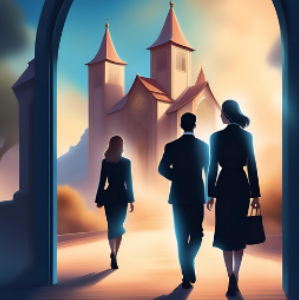
\includegraphics[width=2.625in,height=2.59375in]{media/image5.png}

Die Tage nach ihrem Abendessen schienen von einer besonderen Spannung
durchzogen zu sein, die Anna in jeder Begegnung mit Leonhard spürte.
Ihre Gespräche, die zunächst nur beiläufig und professionell wirkten,
gewannen eine Tiefe, die sie überraschte. Es war, als hätte sich ein
unsichtbarer Faden zwischen ihnen gespannt, der sie bei jeder
Unterhaltung ein Stück näher zueinander zog.

Eines Nachmittags saßen sie in Annas Glaskabine, die Bildschirme
flimmerten mit den Datenströmen vor ihnen. Die Geräusche der Serverräume
waren wie das Summen einer fernen Welt, die in der Stille ihrer
Zusammenarbeit kaum noch von Bedeutung war. Anna lehnte sich vor, die
Finger flogen über die Tastatur, während sie eine Anomalie im Netzwerk
untersuchte.

„Es gibt immer mehr dieser kleinen Abweichungen,`` murmelte sie, während
sie die Datenpakete genauer analysierte. „Fast so, als würde jemand
absichtlich versuchen, die Überwachungssysteme zu umgehen.``

Leonhard beugte sich näher zu ihr, sein Blick folgte den Zahlenreihen,
die über den Bildschirm flossen. „Vielleicht gibt es tatsächlich
jemanden, der nach Schlupflöchern sucht. Oder es ist einfach nur ein
Fehler im Algorithmus -- so perfekt, wie sie behaupten, ist die KI
nicht.``

Seine Worte klangen beiläufig, doch Anna konnte eine subtile Betonung in
seiner Stimme hören, die sie neugierig machte. „Du glaubst also nicht,
dass die Überwachung allmächtig ist?{\kern0pt}`` fragte sie, während sie
versuchte, ihre Skepsis zu verbergen.

„Kein System ist unfehlbar,`` antwortete Leonhard, seine Augen blieben
auf den Bildschirm gerichtet, aber sie spürte, dass seine Gedanken ganz
bei ihr waren. „Es gibt immer eine Lücke, irgendwo. Man muss nur wissen,
wie man sie findet.``

Anna nickte langsam, und ein Gedanke begann in ihr zu keimen -- eine
Idee, die sie gleichzeitig faszinierte und ängstigte. „Was, wenn wir
eine eigene Lücke schaffen könnten?{\kern0pt}`` fragte sie leise, als ob
sie befürchtete, dass die Wände selbst lauschen könnten. „Ein
Kommunikationskanal, der den Überwachungsalgorithmen
entgeht?{\kern0pt}``

Leonhard drehte sich leicht zu ihr um, und sein Lächeln war sowohl
herausfordernd als auch ermutigend. „Quantenverschlüsselung,`` sagte er
fast flüsternd, als wäre dies das Codewort, das eine neue Welt eröffnen
könnte. „Die Quantencomputer des ETZ sind mächtig genug, um solche
Nachrichten zu dekodieren. Aber wenn wir die richtige Methode finden,
könnte es tatsächlich gelingen, einen Kanal aufzubauen, der unbemerkt
bleibt.``

Anna spürte, wie eine Welle der Aufregung durch sie hindurchging. Die
Möglichkeit, ein Kommunikationsnetzwerk zu schaffen, das sich der
Kontrolle entzog, war mehr als nur eine technische Herausforderung -- es
war ein Zeichen von Hoffnung. „Wir könnten das als Experiment tarnen,``
schlug sie vor, ihre Stimme war nun selbstbewusster. „Ein
Forschungsprojekt zur Verbesserung der Sicherheitsprotokolle, offiziell
jedenfalls.``

Leonhard nickte, und seine Augen funkelten vor Begeisterung. „Und
inoffiziell schaffen wir eine Möglichkeit, unabhängig zu
kommunizieren.``

Die Idee begann Gestalt anzunehmen, während sie gemeinsam über die
Details nachdachten, die Algorithmen entwarfen und die Sicherheitslücken
analysierten. Jedes Gespräch, jeder gemeinsam verbrachte Moment brachte
sie ein Stück näher aneinander, aber auch näher an die gefährliche
Realität, dass sie etwas erschaffen wollten, das über die Regeln
hinausging, die ihre Welt bestimmten.

Es war ein riskanter Plan, und doch fühlte es sich für Anna plötzlich
lebendiger an als alles andere, was sie je getan hatte. Sie bemerkte,
dass ihre Blicke sich immer häufiger begegneten, dass die Nähe zwischen
ihnen nicht nur auf ihre gemeinsame Arbeit zurückzuführen war. Es war
ein unausgesprochener Bund, der nicht nur aus Neugier, sondern auch aus
einer leisen Rebellion gegen die mechanische Gleichförmigkeit ihrer Welt
bestand.

In den folgenden Tagen arbeiteten sie oft spät. Während der Rest des ETZ
allmählich zur Ruhe kam, saßen sie in den stillen Stunden der Nacht über
ihre Pläne gebeugt, die Gesichter von den Bildschirmen beleuchtet,
während ihre Finger in der Dunkelheit über die Tastaturen huschten. Es
gab Momente, in denen sich ihre Hände zufällig berührten, kleine,
bedeutungsvolle Berührungen, die ein Gefühl von Vertrautheit weckten,
das sie sich kaum einzugestehen wagten.

Anna fühlte, dass sich etwas Größeres zusammenbraute, eine Veränderung,
die sowohl in ihrer Arbeit als auch in ihrem Leben spürbar war. Es war,
als hätte Leonhard nicht nur den Weg zu einem neuen
Kommunikationsnetzwerk, sondern auch zu ihrem Herzen gefunden -- und sie
wusste, dass sie bald vor der Entscheidung stehen würden, wie weit sie
bereit waren zu gehen.

Leonhard saß allein im abgedunkelten Labor des ETZ, das nur vom
bläulichen Schimmer der Monitoranzeigen und dem sanften Glühen der
leuchtenden Schaltkreise auf dem Arbeitstisch erhellt wurde. Die Uhr
zeigte weit nach Mitternacht, doch für ihn war die Zeit zu einem kaum
wahrnehmbaren Fluss geworden, der sich um die Konzentration seiner
Arbeit wand. Vor ihm lag ein kompliziertes Geflecht aus
Quantenprozessoren, Lasern und optischen Schaltkreisen, die er in den
letzten Wochen behutsam angepasst hatte.

Sein Ziel war es, ein System zu erschaffen, das Quantenverschlüsselung
nicht nur theoretisch anwendbar machte, sondern tatsächlich ein
abhörsicheres Kommunikationsnetzwerk aufbauen konnte. Doch dafür reichte
die bestehende Hardware nicht aus. Er musste die Lichtimpulse in den
optischen Schaltkreisen so präzise synchronisieren, dass sich selbst
kleinste Störungen vermeiden ließen, die von den Überwachungsalgorithmen
registriert werden könnten.

Mit der Spitze eines Schraubendrehers justierte er eine winzige Linse,
die die Lichtwellen durch die schmalen Fasern lenkte. Jeder Handgriff
musste sitzen, denn der kleinste Fehler könnte das gesamte Experiment
zum Scheitern bringen. Die Idee, nachts zu arbeiten, wenn das Labor nur
noch von wenigen Sicherheitskameras überwacht wurde, war riskant -- aber
es war die einzige Möglichkeit, diese geheime Arbeit vor den neugierigen
Augen der Administratoren und den allgegenwärtigen Algorithmen zu
verbergen.

Als Leonhard schließlich den letzten Schaltkreis überprüfte, machte sich
eine Erleichterung in ihm breit. Die ersten Tests zeigten, dass seine
Modifikationen die Interferenzen verringert und die Leistung des Systems
gesteigert hatten. Die Hardware war jetzt in der Lage, verschlüsselte
Signale zu senden und zu empfangen, ohne dass die Standardalgorithmen
von InSim die verschlüsselten Muster erkennen würden. Zumindest in der
Theorie.

Nun kam der kritische Teil: Es musste getestet werden -- und dafür
brauchte er Annas Hilfe. Ihr Wissen über die Netzwerkstrukturen und die
Algorithmen würde sicherstellen, dass sie alle möglichen
Erkennungsmechanismen umgingen. Es war ein gewagter Plan, aber wenn es
funktionierte, würden sie ein Kommunikationssystem erschaffen, das eine
unsichtbare Brücke zwischen den Knotenpunkten des Überwachungsnetzwerks
schlug.

Leonhard lehnte sich zurück und atmete tief durch. Dann griff er nach
seinem Tablet und verfasste eine kurze Nachricht an Anna:

"Treffen wir uns um Mitternacht im Labor? Ich habe etwas, das wir
ausprobieren sollten. Es könnte riskant sein, aber ich denke, es ist der
richtige Moment."

Mit einem letzten Blick auf die nun stillen Schaltkreise sendete er die
Nachricht ab und spürte, wie sein Herz schneller schlug. Er wusste, dass
er Anna in eine gefährliche Situation brachte, doch er vertraute auf
ihre Entschlossenheit und ihren Mut. Wenn jemand diesen Test erfolgreich
durchführen konnte, dann sie beide -- zusammen.

Leonhard blieb einen Moment im gedämpften Licht sitzen, während die
Nachricht an Anna auf dem Bildschirm verblasste. Die leise Summen der
Lüfter in den Rechnern und das leise Knistern der Elektronik verstärkten
die Stille, die in dem verlassenen Labor herrschte. Seine Finger ruhten
auf der Tischkante, während er versuchte, die aufkommende Nervosität zu
verdrängen. Es war nicht das erste Mal, dass er außerhalb der regulären
Arbeitszeiten heimlich experimentierte, aber diesmal stand mehr auf dem
Spiel.

Er stand auf, streckte seine müden Glieder und ging zur Labortür, um
sicherzustellen, dass sie von innen verriegelt war. Danach kehrte er zum
Arbeitstisch zurück und betrachtete die neue Anordnung der Hardware. Das
System, das er aufgebaut hatte, bestand aus einem Quantenknoten, der in
der Lage war, Photonen zu verschränken und ihre Zustände zu verändern,
ohne dass sie von den Standardprotokollen erfasst wurden. Er hatte die
optischen Verbindungen verstärkt, die Laser neu kalibriert und ein
Interferenzmuster eingestellt, das so einzigartig war, dass es wie eine
digitale Signatur wirkte.

Ein letzter Blick auf die Sicherheitskameras zeigte, dass der
Bewegungsmelder im Korridor vor dem Labor nichts Außergewöhnliches
registriert hatte. Alles schien ruhig, und es würde noch eine Weile
dauern, bis die nächtliche Routinekontrolle des Wachpersonals vorbeizog.
Zeit genug für einen ersten Testlauf -- und um zu sehen, ob das System
wirklich so funktionierte, wie er es sich vorstellte.

Mit einer raschen Handbewegung aktivierte er die verschränkten
Photonenquellen und beobachtete, wie die Anzeigen auf dem Bildschirm
aufleuchteten. Die ersten Signale erschienen als komplexe Muster aus
Licht und Schatten, die über die Anzeige tanzten, während die
Photonenpaare ihre Zustände austauschten. Es sah aus, als ob ein
geheimnisvolles Gespräch im Gange wäre, verborgen vor den neugierigen
Augen der Welt.

Leonhard legte die Kopfhörer an und hörte dem leisen Summen und Klicken
der Hardware zu, während er die Signale auf Unregelmäßigkeiten
überprüfte. Es war ein Tanz der Präzision, bei dem jeder Takt stimmen
musste, damit das System reibungslos lief. Die Algorithmen, die er
programmiert hatte, suchten nach jedem noch so kleinen Rauschen, das auf
eine unerwartete Entdeckung hindeuten könnte. Doch bisher schienen die
Signale stabil zu bleiben.

Der Erfolg des Tests ließ seine Anspannung kurz nach, doch die Ruhe war
nur von kurzer Dauer. Ein schrilles Piepen unterbrach den gleichmäßigen
Klang der Geräte -- ein Indikator für eine kleine Anomalie in der
Übertragung. Leonhard runzelte die Stirn und überprüfte die Parameter.
Es war nichts Ernstes, nur eine winzige Abweichung in der Polarisation
eines der Photonen. Eine Korrektur an der Justierung der Lasereinheit
sollte das Problem beheben.

Gerade als er die Einstellungen anpasste, öffnete sich mit einem leisen
Zischen die Tür zum Labor, und Anna trat ein. Sie trug ihren Mantel noch
über der Schulter, die Haare leicht zerzaust vom nächtlichen Wind, der
sie auf dem Weg hierher begleitet hatte. Ihre Augen glitzerten im
Halbdunkel, und für einen kurzen Moment stand sie unschlüssig in der
Tür, als würde sie die geheime Szenerie auf sich wirken lassen.

"Ich dachte, ich wäre die Einzige, die nachts heimlich hier ist", sagte
sie mit einem leichten Lächeln, während sie langsam näher trat. "Du hast
mir ja gar nicht gesagt, dass du ein Geheimlabor hast."

Leonhard erwiderte das Lächeln und deutete auf die Schaltkreise und
Monitore. "Ich habe es wohl improvisiert", antwortete er. "Aber ich
brauche deine Hilfe. Ich glaube, wir haben hier etwas, das funktionieren
könnte -- eine Möglichkeit, uns unsichtbar zu machen. Jedenfalls für die
Überwachungsalgorithmen."

Anna trat näher an den Arbeitstisch heran und beugte sich über die
Hardware, ihre Finger glitten leicht über die verschränkten
Glasfaserkabel und die Photonenquellen. "Du denkst also, wir könnten ein
Netzwerk aufbauen, das außerhalb des regulären Systems läuft?" Sie hob
den Kopf und sah ihn an, eine Mischung aus Neugier und Ernst in ihrem
Blick.

Leonhard nickte. "Das ist die Idee. Aber wir müssen es gründlich testen
-- und das Risiko besteht, dass wir entdeckt werden. Wenn du es nicht
riskieren willst, verstehe ich das."

Anna schüttelte leicht den Kopf. "Ich bin hier, oder? Also lass uns
sehen, was wir damit anstellen können."

Leonhard aktivierte das System erneut, und Anna beobachtete, wie die
Lichter der Geräte nacheinander aufleuchteten. Es war, als würden sie
sich gegenseitig zum Leben erwecken, ein Netzwerk aus geheimen Signalen,
das sich durch den Raum spannte. Die kleinen Anzeigen auf den Monitoren
begannen zu flackern, während die Algorithmen die Datenströme
analysierten und die ersten verschlüsselten Pakete aussandten. Die
Testübertragung war nur ein harmloser Nachrichtentext -- ein Zitat aus
einem alten Gedicht, das Leonhard als Testnachricht gewählt hatte: Die
Freiheit liegt nicht in der Welt, sondern in unseren Herzen.

Anna setzte sich neben Leonhard an den Arbeitstisch, und sie öffneten
gemeinsam die Programmieroberfläche, um den Code durchzugehen. Die Luft
im Labor war kühl, und die Dunkelheit draußen verlieh dem Raum eine
abgeschottete Atmosphäre, in der sich die Geräusche der Geräte noch
deutlicher abzeichneten. Der leise Rhythmus des summenden Lüfters schien
zu einem Begleiter ihrer Gedanken zu werden, während sie in das Netz aus
mathematischen Formeln und verschlüsselten Signalen eintauchten.

„Schau hier``, sagte Leonhard leise und deutete auf eine Stelle im Code.
„Das sind die aktuellen Protokolle der Überwachungssysteme. Wir haben
gerade ein Datenpaket verschickt, das theoretisch registriert werden
müsste -- aber es taucht in keiner der Kontrollspuren auf.``

Anna sah ihn nachdenklich an. „Das heißt, wir haben es geschafft, uns
unter dem Radar zu bewegen. Aber was, wenn sie die Parameter ändern? Sie
könnten die Algorithmen anpassen, wenn sie eine Anomalie entdecken.``

„Deshalb müssen wir sicherstellen, dass unser Signal nicht nur
unsichtbar ist, sondern auch wie etwas anderes aussieht``, entgegnete
Leonhard. „Ich arbeite an einer Methode, bei der die
Quantenverschlüsselung nicht nur als Rauschen getarnt wird, sondern auch
andere Muster erzeugt, die in den bestehenden Datenstrom eingebettet
werden.``

Anna nickte. „Das könnte klappen, aber dafür brauchen wir mehr
Rechenleistung, als wir hier haben. Vielleicht könnten wir die
Rechenkapazitäten anderer Labore unauffällig nutzen, ohne Verdacht zu
erregen.``

Leonhard hob den Blick und lächelte schief. „Ein nächtlicher
Datenraubzug in den Servern der Nachbarlabore? Das klingt nach einer
Herausforderung.`` Er lehnte sich zurück und beobachtete Anna, wie sie
konzentriert über den Code nachdachte. „Aber bevor wir das angehen,
sollten wir sicherstellen, dass unser kleiner Testlauf hier wirklich
stabil ist. Bist du bereit für eine größere Übertragung?{\kern0pt}``

Anna nickte entschlossen, ihre Augen funkelten im schwachen Licht der
Monitore. „Lass es uns versuchen. Wenn wir entdeckt werden, dann
wenigstens, weil wir etwas Großes wagen.``

Sie gaben die Befehle für die nächste Testsequenz ein und schickten ein
deutlich umfangreicheres Datenpaket ab, während die Uhr in der Ecke des
Bildschirms die Minuten herunterzählte. Jede Sekunde fühlte sich an wie
eine kleine Ewigkeit, als sie auf die Rückmeldungen des Systems
warteten. Das Brummen der Geräte schien lauter zu werden, die Lichter
auf den Monitoren leuchteten greller, und die Anzeigen begannen sich in
einem neuen Muster zu bewegen -- ein Zeichen, dass die Übertragung
tatsächlich unentdeckt geblieben war.

Ein leiser Aufatmen ging durch den Raum, und Anna und Leonhard tauschten
einen kurzen Blick aus. Es war mehr als nur der Triumph über den
erfolgreichen Test -- es war das erste gemeinsame Abenteuer, eine
geheime Allianz, die sie mit jedem Tastendruck und jedem Risiko stärker
miteinander verband.

„Jetzt sollten wir wohl verschwinden, bevor die Sicherheitsleute hier
auftauchen``, sagte Anna mit einem Grinsen, während sie ihre Sachen
zusammenpackten. „Oder hast du noch etwas im Ärmel, das wir sofort
ausprobieren müssen?{\kern0pt}``

Leonhard schüttelte den Kopf. „Das war genug Nervenkitzel für eine
Nacht. Aber vielleicht sollten wir morgen Abend über das weitere
Vorgehen sprechen -- irgendwo außerhalb des Labors, wenn du Lust hast.``

Anna warf ihm einen schelmischen Blick zu. „Vielleicht, aber lass uns
jetzt lieber gehen, bevor wir wirklich noch auffallen.``

Gemeinsam verließen sie das Labor, ihre Schritte hallten in dem dunklen
Flur wider, während sie durch die verlassenen Korridore eilten. Der
erste Schritt war getan -- das unsichtbare Netzwerk existierte nun
zumindest in ihren Köpfen, und sie wussten, dass sie auf etwas gestoßen
waren, das ihre Arbeit im ETZ weit hinter sich ließ.

Der nächste Abend brach an, und die Stadt erwachte in der Dämmerung zum
Leben. Anna und Leonhard schlenderten durch die breiten Straßen des
Stadtzentrums, vorbei an gläsernen Hochhäusern und elektronischen
Werbetafeln, die im Rhythmus der Musik flimmerten. Die Lichter der Stadt
hüllten die Welt in ein kaleidoskopisches Glitzern, und das Summen der
Drohnen, die in der Luft patrouillierten, mischte sich mit dem Murmeln
der Passanten.

„Wohin wollen wir?{\kern0pt}``, fragte Leonhard, während sie an einer
Vielzahl kleiner Bars und Restaurants vorbeigingen. „Ein ruhiges
Plätzchen wäre jetzt genau das Richtige.``

Anna nickte zustimmend, und sie steuerten eine kleine Weinbar an, deren
gedämpftes Licht und sanfte Jazzmusik eine wohltuende Abwechslung zur
Hektik draußen boten. Sie setzten sich an einen Tisch in einer
gemütlichen Ecke, und Anna öffnete die Menükarte auf dem holographischen
Display, das aus der Tischplatte aufleuchtete.

„Ich lade dich ein``, sagte Leonhard mit einem freundlichen Lächeln und
hielt seine Hand an den biometrischen Scanner auf der Tischplatte. Ein
leises Summen erklang, und sein digitales Wallet öffnete sich, indem es
die Sicherheitsprüfung durchlief. Sofort erschienen mehrere Anzeigen,
die den aktuellen Status seines Sozialkreditprofils und seiner
Zahlungslimits anzeigten.

„Wow, das nenne ich Service``, bemerkte Anna, als sie die automatischen
Berechnungen des Systems betrachtete. „Du hast einen ziemlich guten
Sozialkredit Score."

„Ja, solange ich die Regeln einhalte und brav lebe``, erwiderte Leonhard
trocken. „Aber das kann sich schnell ändern. Ein paar falsche Klicks,
eine unangemessene Bewegung -- und schon kann das Profil abrutschen.``

Anna nickte. „InSim hat das System in den letzten Jahren stark
verfeinert. Ihre Algorithmen bestimmen nicht nur, was wir kaufen dürfen,
sondern auch, wann wir es kaufen. Sie passen die Preise dynamisch an
unsere Kreditwerte an.``

Leonhard lehnte sich in seinem Stuhl zurück und ließ den Blick durch den
Raum schweifen. „Manchmal frage ich mich, wie viel von den Gesetzen, an
die wir uns halten, wirklich von Menschen erdacht wurde -- oder ob die
Algorithmen, die bei InSim laufen, nicht längst auch darüber
entscheiden. Es heißt immer, die Richtlinien würden nur automatisiert
durchgesetzt, aber ich habe meine Zweifel.``

Anna stimmte zu. „Die Anpassungen im Regelwerk erfolgen so schnell, dass
es kaum möglich ist, die Änderungen nachzuvollziehen. Es ist, als würden
wir einem ständig wechselnden Bild folgen, das sich mit jeder Bewegung
verzieht. Die gesetzgebenden Algorithmen agieren wie ein sich selbst
veränderndes System, das uns Menschen als Variablen betrachtet -- keine
Subjekte, sondern bloße Datenpunkte.``

In diesem Moment brachte der Serviceroboter ihre Getränke, und Anna
hielt ihr Glas mit Rotwein hoch. „Auf uns``, sagte sie, „und darauf,
dass wir vielleicht eines Tages einen Weg finden, diesen
Algorithmusfesseln zu entkommen.``

Leonhard hob ebenfalls sein Glas und prostete ihr zu. „Auf uns -- und
auf die Freiheit, die wir in den verschlüsselten Netzwerken suchen.
Manchmal denke ich, es ist ironisch, dass wir versuchen, einen Fluchtweg
aus den gleichen Algorithmen zu finden, die wir für unsere Zwecke nutzen
wollen.``

„Ironisch, aber auch genau der Punkt``, antwortete Anna. „Wir wissen,
wie die Systeme funktionieren, wir kennen ihre Schwächen. Wenn wir
vorsichtig sind, können wir die Quantenverschlüsselung nutzen, um
Nachrichten zu senden, die völlig im Rauschen untergehen. Ein Netzwerk,
das sich innerhalb der Datenströme verbirgt, unsichtbar und unerreichbar
für InSim.``

„Genau``, stimmte Leonhard zu. „Das ist der Plan. Aber zuerst sollten
wir die Nacht genießen, bevor wir uns wieder an die Arbeit machen.``

Die beiden lächelten sich an und tranken, während die Musik
weiterspielte und die Welt draußen in einem ständigen Tanz aus Licht und
Schatten pulsierte. Doch unter dem scheinbar sorglosen Abend lag die
unausgesprochene Gewissheit, dass jeder Schritt auf einem schmalen Grat
verlief -- einem Grat zwischen Freiheit und totaler Kontrolle.

Spät in der Nacht, als die Gänge des ETZ still und verlassen waren,
kehrten Anna und Leonhard zurück ins Labor. Ihre Schritte hallten auf
dem kalten Boden wider, und die wenigen aktiven Überwachungskameras
registrierten lediglich ihre Anwesenheit, ohne auf die ungewöhnliche
Uhrzeit zu reagieren. Sie hatten die Sicherheitsprotokolle mit einem
kleinen Trick umgangen, sodass ihr Zugang als eine gewöhnliche
Wartungsaufgabe vermerkt wurde.

„Jetzt wird es spannend``, murmelte Leonhard, als sie vor den
Arbeitsstationen standen, die im schwachen Licht der Monitore
schimmerten. Sie hatten alles vorbereitet: Eine modifizierte Hardware
Platine, die als Quantenverschlüsselungsmodul diente, war an das
Netzwerk angeschlossen, bereit, ihre verschlüsselten Nachrichten ins
Herz von InSims Infrastruktur zu schicken.

Anna setzte sich an eine der Konsolen und tippte den letzten Befehl ein,
der das System startete. „Das ist der Moment der Wahrheit. Wenn wir
unentdeckt bleiben, können wir den gesamten Datenstrom nutzen, ohne dass
irgendjemand etwas merkt.`` Ihre Stimme klang angespannt, und ihre
Finger zitterten leicht, als sie die Eingabetaste drückte.

Ein leises Brummen erfüllte den Raum, als die Platine auf Hochtouren
lief und ihre komplexen Quantenberechnungen durchführte. Auf den
Monitoren erschienen Datenpakete, die scheinbar harmlos im Netzwerk
kursierten. Das System sandte ihre verschlüsselten Nachrichten aus,
eingebettet in die alltägliche Kommunikation, die zwischen den
verschiedenen Knotenpunkten von InSim ausgetauscht wurde.

„Da``, sagte Leonhard, seine Augen glänzten vor Aufregung. „Schau dir
das an -- unsere Pakete bewegen sich direkt durch das InSim Netzwerk.
Sie sind vollständig getarnt, eingebettet in den Strom der offiziellen
Daten. Es gibt keine Anzeichen dafür, dass sie irgendjemand bemerkt.``

Anna lehnte sich nach vorne, während sie die Bewegungen auf dem
Bildschirm verfolgte. „Wir haben es tatsächlich geschafft``, sagte sie
leise, fast ehrfürchtig. „Wir sind huckepack auf dem InSim Netzwerk
unterwegs, und niemand weiß davon. Unsere Nachrichten sind für die
Algorithmen nichts weiter als Rauschen.``

Leonhard lächelte. „Das ist der erste Schritt. Wenn wir das stabil
halten können, haben wir ein Kommunikationsnetzwerk, das unauffindbar
ist -- eine Grundlage für all das, was wir planen.``

Anna nickte, doch ihre Gedanken wanderten bereits weiter. „Wir müssen es
ausbauen, testen, sicherstellen, dass es keine Lücken gibt. Die
Algorithmen bei InSim sind nicht dumm; sie passen sich an. Es wird nicht
lange dauern, bis sie versuchen, Anomalien im Datenverkehr zu
erkennen.``

„Stimmt``, stimmte Leonhard zu. „Aber bis dahin haben wir vielleicht
schon die nächste Entwicklung in der Hand. Ein verschlüsseltes Netz ist
nur der Anfang. Wir brauchen auch eine sichere Möglichkeit,
Informationen zu speichern und zu verarbeiten. Irgendwo, wo InSim nicht
hinkommt.``

Sie tauschten einen kurzen Blick aus, beide ergriffen von dem Gefühl, an
der Schwelle zu etwas Großem zu stehen. Ihre Entdeckung eröffnete völlig
neue Möglichkeiten, und gleichzeitig lag die Gefahr wie ein Schatten
über ihren Plänen. Sie wussten, dass es nur eine Frage der Zeit war, bis
InSim von ihrer Existenz erfuhr.

Doch in diesem Moment, in der Stille des Labors und mit der Dunkelheit
der Nacht um sie herum, fühlte sich alles möglich an. Sie hatten einen
Weg gefunden, die allgegenwärtigen Algorithmen zu umgehen, zumindest
vorübergehend, und das allein war bereits ein gewaltiger Schritt in
Richtung Freiheit.

Ein halbes Jahr verging, in dem Anna und Leonhard an verschiedenen
Fronten beschäftigt waren, aber ihre gemeinsame Arbeit am
Verschlüsselungssystem blieb ein ständiger Anker. Ihre Beziehung
entwickelt sich langsam, angereichert durch kleine Momente, in denen
ihre Verbindung deutlicher wurde.

Leonhard verbrachtet einige Wochen im Krankenhaus, nachdem ein harmloser
Unfall beim Sport eine alte Verletzung aufgerissen hatte. Während dieser
Zeit blieb Anna mit ihm in Kontakt und nutzte das Netzwerk, um ihm
verschlüsselte Nachrichten zu senden, die nicht nur technische Updates,
sondern auch kleine Rätsel oder sogar Botschaften mit versteckten
persönlichen Anspielungen enthielten. Es begann als ein harmloser Spaß,
aber im Laufe der Zeit wurde deutlich, dass ihre Nachrichten immer
intimer und persönlicher wurden. Leonhard freute sich jedes Mal, wenn er
eine neue Nachricht von Anna entdeckte, und begann, sie als eine Art
Spiel zu sehen, bei dem sie sich langsam gegenseitig öffneten.

In dieser Phase wurde beiden auch deutlicher, wie die Stadt und das
InSim System den Alltag kontrollieren. Jeder Besuch im Krankenhaus, jede
Anwendung im Alltag wird getrackt, bewertet und fließt in das
persönliche Sozialkredit Ranking ein. Einmal erfuhr Leonhard durch
Zufall, dass sein Krankenstand seine Punkte negativ beeinflusste, was
ihn weiter von bestimmten Annehmlichkeiten der Stadt ausschloß.

Nach Leonhards Entlassung treffen sich die beiden wieder regelmäßig im
Labor. Sie erweitern ihr Verschlüsselungssystem, indem sie neue
Anwendungen entwickeln und sich selbst Herausforderungen stellen.
Leonhard, der die technischen Details liebt, erfindet eine Art
Schnitzeljagd, bei der die nächste Nachricht immer erst nach der Lösung
eines vorherigen Rätsels auftaucht, und versteckt die Nachrichten an
verschiedenen Orten in der Stadt -- auf den Werbetafeln, in Codes, die
scheinbar harmlose digitale Poster an Bushaltestellen enthalten.

Diese gemeinsamen „Abenteuer`` lassen die Stadt für sie in neuem Licht
erscheinen. Sie erleben, wie man trotz der allgegenwärtigen Kontrolle
eine Art Spielraum schaffen kann, um sich gegen die systematische
Überwachung zu wehren. Und während sie den Spuren folgen und Nachrichten
entschlüsseln, geschehen Dinge, die ihre Nähe weiter vertiefen: Ein
kurzer Händedruck, der länger dauert, als es nötig wäre, ein
verstohlener Blick, der nicht ganz rechtzeitig abgewendet wird.

Bei einem Abendessen diskutieren sie über das Überwachungs und
Kreditsystem, das jeden Aspekt ihres Lebens regelt. Es kommt zur
Sprache, dass manche Bürger sich virtuelle Partner schaffen, um ihr
emotionales Leben „aufrechtzuerhalten``, da der physische Kontakt in der
technokratischen Gesellschaft oftmals als unpraktisch gilt. Diese
künstlichen Beziehungen sind von InSim kontrolliert, um die emotionalen
Bedürfnisse der Menschen zu kanalisieren und zu manipulieren.

Anna und Leonhard machen sich darüber lustig, wie Algorithmen die Regeln
für Intimität und Nähe bestimmen, und fühlen eine subtile Auflehnung in
sich aufsteigen. Diese Diskussion über virtuelle Partnerschaften führt
dazu, dass sie die Grenze zwischen Spiel und Ernsthaftigkeit in ihren
Gesprächen verschieben und langsam mehr wagen. Doch echte Berührungen
und gemeinsame Erlebnisse füllen nach und nach die Lücken, die
künstliche Verbindungen nie ausgleichen könnten.

\section{Die Entdeckung von ARS}\label{die-entdeckung-von-ars}

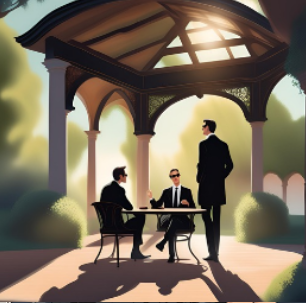
\includegraphics[width=2.73958in,height=2.76042in]{media/image4.png}

Die ersten echten Tests mit dem verschlüsselten Netzwerk zeigen Lücken
in der Sicherheit. Einmal wird eine ihrer verschlüsselten Nachrichten
abgelehnt, weil das InSim Netzwerk unerwartet reagiert hat. Diese
Rückschläge verlangsamen ihre Fortschritte, geben aber auch Hinweise auf
die genaue Funktionsweise des Systems. In den nächsten Wochen verbringen
sie oft Nächte im Labor, um Fehler zu beheben und neue Methoden
auszuprobieren, immer wieder auf der Suche nach dem perfekten
Schlupfloch, um die Überwachung zu umgehen.

Während einer dieser Nächte, erschöpft und frustriert nach mehreren
Fehlversuchen, passiert etwas Unerwartetes. Leonhard lehnt sich zurück
und lässt eine Bemerkung über „unrealistische Erwartungen`` fallen --
nicht nur über das Netzwerk, sondern auch über das Leben in der City und
vielleicht sogar über ihre unausgesprochene Verbindung. Anna erwidert
seinen Blick, und es ist, als würde die Luft für einen Augenblick
stillstehen. Aber anstatt die Spannung zu lösen, machen sie einfach
weiter mit ihrer Arbeit. Beide wissen, dass sich da etwas anbahnt, auch
wenn es in diesem Moment nicht ausgesprochen wird.

So ziehen die Tage hin und jeder Morgen bringt den nächsten Tag. Die
kühle Brise eines dieser frühen Morgen wehte durch die offenen Fenster
des InSim-Büros und mischte sich mit dem Geruch von frischem Kaffee, der
durch den Raum zog. Anna saß an ihrem Arbeitsplatz, ihre Augen auf den
Bildschirm gerichtet, während sie sich Notizen für die bevorstehenden
Projekte machte. Die monotonen Töne der Computertastatur wurden jäh
durch das Geräusch eines Klopfens unterbrochen, gefolgt von dem
vertrauten Gesicht ihres Vorgesetzten, der den Raum betrat.

„Guten Morgen, Anna. Ist Leonhard schon da?{\kern0pt}`` fragte er, seine
Stimme klang sowohl geschäftsmäßig als auch leicht aufgeregt.

„Er sollte gleich kommen,`` antwortete Anna und warf einen Blick auf die
Uhr. „Was gibt es denn?{\kern0pt}``

Kaum hatte sie die Worte ausgesprochen, öffnete sich die Tür und
Leonhard trat ein, die Haare zerzaust und ein breites Grinsen im
Gesicht. „Entschuldigung, ich musste noch schnell einen Bericht
fertigstellen,`` sagte er und ließ sich in den Stuhl neben Anna fallen.

Ihr Vorgesetzter trat näher und stellte einen holprigen Datenstick auf
den Tisch. „Wir haben einen neuen Auftrag für euch,`` begann er, während
er die beiden neugierig musterte. „Es geht um die Überprüfung alter
Datenarchive in einem verlassenen InSim-Datenzentrum.``

„Ein Datenzentrum? Das klingt spannend! Wo ist es?{\kern0pt}`` Leonhards
Augen leuchteten vor Neugier, und er war sofort bereit, sich ins
Abenteuer zu stürzen.

„Es befindet sich am Rande der Stadt, in einem Viertel, das seit Jahren
nicht mehr betreten wurde. Die Berichte über das Zentrum deuten darauf
hin, dass dort noch wertvolle Informationen lagern -- Informationen, die
uns helfen könnten, die Effizienz und Kreativität eurer bisherigen
Zusammenarbeit weiterzuführen.``

Anna spürte ein Kribbeln in ihrem Bauch. Die Vorstellung, alte Archive
zu durchforsten, erweckte in ihr den Forschergeist. „Gibt es spezielle
Auflagen für diesen Auftrag?{\kern0pt}`` fragte sie, während sie sich
eine lange Liste von Möglichkeiten durch den Kopf gehen ließ.

„Das übliche. Seid vorsichtig, haltet euch an die Sicherheitsrichtlinien
und vergesst nicht, regelmäßig Bericht zu erstatten. Aber ich denke,
dass ihr das meistern werdet.`` Der Vorgesetzte lächelte und nickte
ermutigend. „Das Datenzentrum ist veraltet und könnte einige
Überraschungen bereithalten. Ich vertraue darauf, dass ihr das Beste
daraus macht.``

Nachdem er den Raum verlassen hatte, warf Anna einen Blick auf Leonhard.
„Das wird großartig! Stell dir vor, welche Geschichten die alten Daten
erzählen könnten.``

„Ich kann es kaum erwarten! Lass uns gleich einen Plan machen und
loslegen!{\kern0pt}``

Sie begannen, die notwendigen Vorbereitungen zu treffen. Mit jedem
Schritt, den sie in Richtung des unbekannten Ziels machten, spürten sie
die Aufregung in der Luft. Es war mehr als nur ein Auftrag. Es war eine
Gelegenheit, in die vergessenen Winkel der digitalen Vergangenheit
einzutauchen, eine Schatzsuche im Schatten der Technologie, und die
beiden waren bereit, jede Herausforderung anzunehmen.

Anna und Leonhard nahmen im Transporter Platz, der sie zur alten
Kuppelstadt bringen würde. Die Wände des Fahrzeugs waren aus einem
leichten, transparenten Material, das es ihnen erlaubte, die
Stadtlandschaft hinter sich zu sehen, während sie durch die Luft
schwebten. Auf der einen Seite erhoben sich die glänzenden Türme der
Hochhäuser, die das pulsierende Herz der Kuppelstadt ausmachten -- ein
Ort voller Leben, in dem Menschen in hochmodernen Wohnungen lebten,
umgeben von digitalen Annehmlichkeiten.

„Schau dir die Wohnviertel an,`` sagte Anna und deutete auf die
leuchtenden Fassaden der Gebäude, die mit lebendigen Projektionen
geschmückt waren. „So viele Menschen, die in diesen eleganten Strukturen
leben. Es wirkt fast perfekt.``

Leonhard nickte zustimmend und beobachtete die unzähligen Balkone, auf
denen Pflanzen in vertikalen Gärten wuchsen. „Es ist erstaunlich, wie
InSim alles gestaltet hat. Sie haben ein ganz eigenes Ökosystem
geschaffen -- ein bisschen wie ein futuristisches Paradies.``

Der Transporter hob ab und schwebte über die verschiedenen Stadtteile
hinweg. Unter ihnen erstreckten sich die landwirtschaftlichen Zonen, wo
Gewächshäuser in harmonischen Reihen angeordnet waren. Die Pflanzen, die
dort wuchsen, waren alle durch holographische Anzeigen sichtbar, die den
Fortschritt des Anbaus anzeigten.

„Die Menschen hier leben in einer perfekten Illusion,`` murmelte Anna
nachdenklich. „Sie glauben, dass alles gut ist, aber was ist mit denen,
die am Rande der Stadt leben?{\kern0pt}``

„Gute Frage,`` erwiderte Leonhard, während sie an einem Stadtviertel
vorbeifuhren, das sich stark von den glänzenden Hochhäusern abhob. Die
heruntergekommenen Gebäude waren aus grauem Beton, und die Fenster waren
größtenteils zerbrochen. In den Straßen tummelten sich Menschen, deren
Kleidung abgetragen und schmutzig war. „Das ist der Slum. Kaum jemand
spricht über diese Teile der Stadt.``

„Es ist schockierend, wie sehr InSim die Stadt nach außen hin
inszeniert, während sie die dunkleren Ecken versteckt,`` fügte Anna
hinzu. „Was würde hier passieren, wenn die Technologie
ausfällt?{\kern0pt}``

Der Transporter setzte seine Reise fort und überflog die
Produktionszonen, wo riesige Fabriken unermüdlich arbeiteten. Roboter
bewegten sich geschäftig zwischen den Maschinen, während die Lichter in
rhythmischem Takt blinkten. „Es ist wie ein riesiges Uhrwerk, das
ununterbrochen tickt. Was, wenn jemand das System stört?{\kern0pt}``
fragte Leonhard und seine Stimme verriet eine Mischung aus Bewunderung
und Besorgnis.

„Es ist faszinierend und beängstigend zugleich,`` sagte Anna. „All diese
Technik, die unsere Gesellschaft antreibt, könnte auch ihre größte
Schwäche sein.``

Plötzlich tauchte die Ruine des alten InSim-Datenzentrums vor ihnen auf,
eingehüllt in Schatten und umgeben von überwuchertem Gras. Die Kontraste
zwischen der lebhaften Stadt und diesem verfallenen Ort waren so
auffällig, dass es fast surreal wirkte.

„Da ist es!{\kern0pt}`` rief Anna und deutete auf das verwitterte
Gebäude, das einst ein Zentrum des Wissens und der Macht gewesen sein
musste. „Ein Ort, der die Geheimnisse der Vergangenheit birgt.``

Der Transporter setzte sanft auf der Plattform vor dem Datenzentrum auf,
und die beiden stiegen aus. Die Kuppelstadt schien in der Ferne zu
pulsieren, während die Dunkelheit des Datenzentrums sie umhüllte. Mit
einem letzten Blick auf die glanzvollen Lichter der Stadt fühlten Anna
und Leonhard ein Knistern in der Luft -- die Vorahnung von Entdeckungen,
die das Potenzial hatten, ihre Welt für immer zu verändern.

Die beiden standen vor dem alten InSim-Datenzentrum, dessen massives
Stahlgerüst wie ein schlafender Riese in der Abenddämmerung wirkte. Das
Gebäude war von einer mystischen Aura umgeben, die die Luft elektrisch
auflud. Anna und Leonhard hielten ihre Zugangskarten in der Hand, die im
schwachen Licht der umstehenden Laternen schimmerten.

„Laut den Aufzeichnungen sollte der Eingang hier irgendwo sein,``
murmelte Anna, während sie um das Gebäude schritt und nach Anzeichen
suchte. „Es fühlt sich an, als ob wir in ein Geheimnis eindringen, das
lange verborgen war.``

Leonhard sah sich um, seine Neugierde wuchs mit jedem Schritt. „Ich
frage mich, welche Art von Informationen hier lagern. Vielleicht Dinge,
die die Menschen vergessen haben -- oder die absichtlich vergessen
wurden.``

„Wir wissen, dass es ungewöhnliche Datenströme gab. Es könnte alles
sein, von vergessenen Technologien bis hin zu den geheimen Plänen von
InSim,`` fügte Anna hinzu. „Aber auch etwas anderes... etwas, das wir
uns noch nicht einmal vorstellen können.``

Sie fanden einen schmalen, fast unsichtbaren Zugang zwischen zwei
verwitterten Betonblöcken. „Hier! Ich glaube, das könnte der Eingang
sein,`` rief Anna aufgeregt und drückte ihre Zugangskarten gegen das
veraltete Terminal.

Ein leises Summen ertönte, gefolgt von einem mechanischen Geräusch, als
die Tür langsam aufschwang und einen dunklen Schlund offenbarte.
„Bereit?{\kern0pt}`` fragte Leonhard, während er einen kurzen Blick auf
Anna warf. Ihr Blick war entschlossen, aber es lag auch eine Spur von
Nervosität darin.

„Ja,`` antwortete sie, „lass uns herausfinden, was hier drin ist.``

Als sie die Schwelle übertraten, erwachte die Energieversorgung des
Datenzentrums wie ein schlafender Drache. Die Wände flackerten mit
neonblauen und grünen Lichtern, während die alten Systeme, die
Jahrzehnte lang inaktiv gewesen waren, wieder zum Leben erwachten. Ein
sanftes Surren erfüllte den Raum, und die Bildschirme an den Wänden
begannen, in unregelmäßigen Abständen zu blitzen.

„Wow, es fühlt sich an, als wären wir die ersten Menschen hier seit
Ewigkeiten,`` flüsterte Leonhard, während sie tiefer in den Raum
vordrangen. „Als ob die Vergangenheit uns beobachtet.``

„Die Geister der Daten, die hier gespeichert sind,`` scherzte Anna, aber
ihre Stimme war leise, als sie die düstere Atmosphäre spürte. „Ich habe
das Gefühl, dass wir auf etwas Großes stoßen werden.``

Sie wagten sich weiter in die Dunkelheit, und die Lichter pulsierten in
einem hypnotischen Rhythmus. Es war, als ob die Mauern selbst
Geschichten flüsterten, die darauf warteten, von ihnen entschlüsselt zu
werden. Der Nervenkitzel des Unbekannten umgab sie, während sie sich in
die Tiefen des Datenzentrums begaben, bereit, die Geheimnisse zu lüften,
die es birgt.

Die Luft im Datenzentrum war still und kühl, wie die eines lange
verlassenen Ortes, und der scharfe Geruch von alten Schaltkreisen und
staubigen Kabeln hing schwer in der Atmosphäre. Das schwache Leuchten
der Notbeleuchtung ließ Schatten über die Reihen aus veralteten
Monitoren und klobigen Servern tanzen. Anna und Leonhard arbeiteten sich
vorsichtig durch den Raum, wobei ihre Schritte auf dem metallenen Boden
ein leises Echo erzeugten. Ihre Augen suchten unablässig nach etwas, das
den langen Weg hierher lohnenswert machen würde.

Schließlich stießen sie auf einen massiven Schrank, dessen metallene Tür
sich unter Annas Zug nur widerwillig mit einem langen, rostigen Knarren
öffnete. Eine Schicht aus Staub wirbelte auf und legte sich wie feiner
Nebel über das Halbdunkel, als das Innere des Schranks zum Vorschein
kam. In seinem tiefen, grauen Schlund lagen übereinandergestapelte
Datenträger, bedeckt von einer dicken Staubschicht, die von vergangener
Zeit zeugte. Ein schwaches Licht schimmerte auf den abgenutzten
Oberflächen und schien sie mit einer seltsamen, unheimlichen Aura zu
umhüllen.

„Schau mal, das hier...`` Annas Stimme klang gedämpft, fast ehrfürchtig,
als sie einen der alten Datenträger herauszog. Die Aufschrift auf dem
metallenen Gehäuse war verblasst, doch der Name „ARS`` stach hervor,
eingeritzt und von Jahren der Vernachlässigung umrahmt. Ihre Finger
zitterten leicht, als sie den Fund in die Höhe hielt und das
abgegriffene Stück Technik neugierig betrachtete. „Es sieht aus, als ob
es etwas mit einer Künstlichen Intelligenz zu tun hat, schau, das InSim
Logo... aber die Informationen scheinen unvollständig.``

Leonhard trat näher heran und starrte auf die alten Schaltkreise, die im
schwachen Licht matt schimmerten. „Könnte das der Schlüssel zu den
Datenanomalien sein, die wir gesehen haben?{\kern0pt}`` fragte er, und
in seinen Augen blitzte die Entschlossenheit auf, das Rätsel zu lösen.
„Vielleicht haben wir mehr gefunden, als wir je erwartet hätten.``

Leonhard beugte sich näher zu dem alten Teil Hardware, und ein Prickeln
lief seinen Rücken hinunter -- die Art von Nervenkitzel, die man spürt,
wenn man kurz davor ist, ein verborgenes Geheimnis zu lüften. Er hielt
das verstaubte Stück Technologie fest in der Hand, während sein Blick
auf den flackernden Bildschirmen vor ihnen verweilte.

„Schau dir das an,`` murmelte er, seine Stimme kaum mehr als ein
Flüstern. Sein Finger zeigte auf die Monitore, auf denen sich eine
seltsame Grafik abzeichnete. Linien und Punkte zuckten über den
Bildschirm wie Blitze am Horizont, formten Wellen, die auf den ersten
Blick chaotisch wirkten, doch bei genauerem Hinsehen eine unheimliche,
organische Struktur offenbarten. Die Datenströme flossen nicht in den
üblichen, geordneten Mustern, sondern pulsierten und verschmolzen
miteinander, als ob sie einem eigenen Rhythmus folgten -- als ob sie
kommunizierten.

„Das sind keine gewöhnlichen Signale,`` sagte er, seine Augen fest auf
die sich bewegenden Linien gerichtet. „Es ist, als ob...`` Er stockte
und suchte nach den richtigen Worten. „... als ob sie leben. Diese
Wellen folgen keiner bekannten Logik, sie scheinen... zu denken, sie
spielen ein Spiel des Lebens.``

Anna trat neben ihn, ihre Neugier geweckt von dem, was sich vor ihren
Augen abspielte. Sie spürte das unterschwellige Knistern in der Luft,
eine Spannung, die sie an die Oberfläche eines stürmischen Meeres
erinnerte, auf dem sie nun trieben, ohne zu wissen, was in der Tiefe
lauern mochte. „Du meinst, sie könnten wirklich miteinander
kommunizieren?{\kern0pt}`` fragte sie, die Faszination in ihrer Stimme
unüberhörbar.

Leonhard nickte langsam, ohne den Blick von den Bildschirmen abzuwenden.
„Irgendetwas stimmt hier ganz und gar nicht,`` murmelte er. „Es ist, als
ob wir den Herzschlag eines Systems belauschen, das längst abgeschaltet
sein sollte.``

Anna trat einen Schritt näher an die flackernden Bildschirme heran, die
Grafik darauf pulsierte in lebhaften Mustern. Ihre Augen folgten den
Linien, die wie kleine Ströme in einem verborgenen Flussnetz über den
Monitor liefen. „Das sieht aus, als ob hier etwas kommuniziert,
vielleicht sogar bewusst Informationen austauscht,`` sagte sie, ihre
Stimme vor Anspannung gedämpft. „Es ist, als ob wir nur einen flüchtigen
Blick auf etwas erhaschen, das absichtlich verborgen wurde.``

Entschlossen setzten sie sich vor die Terminals und begannen, sich durch
die zahllosen Protokolle und Datenprotokolle zu wühlen. Jedes Mal, wenn
sie eine Datei öffneten, tauchten neue, chaotisch wirkende
Informationsströme auf, die einer eigenen, unerklärlichen Logik folgten.
Mit jedem Mausklick, mit jeder neu entschlüsselten Zeile entfalten sich
Schichten aus verschlüsselten Botschaften, fragmentierten Codes und
seltsamen Sequenzen, die aufeinander zu reagieren schienen, als ob eine
unsichtbare Hand sie lenkte.

Je tiefer sie vordrangen, desto komplexer und rätselhafter wurden die
Informationen. Überall tauchten Anomalien auf -- Unstimmigkeiten, die
auf mehr hinzudeuten schienen als nur ein altes, fehlerhaftes System. Es
war, als hätten sie eine Tür geöffnet, die in eine andere Welt führte --
eine Welt aus vergessenen Datenströmen, verlorenem Wissen und
verschleierten Botschaften.

In ihren Gedanken begannen sich die Puzzlestücke zu formieren. Es war
nicht bloß eine Ansammlung seltsamer Dateien; hier schien eine ganze
Geschichte darauf zu warten, ans Licht geholt zu werden -- eine
Geschichte, die niemand je lesen sollte, die absichtlich im Schatten
gehalten wurde. Anna und Leonhard spürten beide, wie ihre Herzen
schneller schlugen. Es war nicht mehr nur ein Auftrag, den sie
auszuführen hatten; es war die Entdeckung eines Mysteriums, das größer
war, als sie es sich je hätten vorstellen können.

Nach stundenlanger, fieberhafter Recherche und der Auseinandersetzung
mit den geheimnisvollen Datenströmen wussten Anna und Leonhard, dass sie
sich auf gefährlichem Terrain befanden. Die Datei „ARS`` hatte sich als
weit mehr als nur eine verstaubte Entdeckung herausgestellt; sie war ein
Rätsel, das sich wie ein dichter Nebel um ihre Gedanken legte. Mit einer
Mischung aus Aufregung und Vorsicht beschlossen sie, den entscheidenden
Schritt zu wagen: Sie würden die KI reaktivieren und herausfinden, was
sich wirklich hinter dem Namen „ARS`` verbarg.

Leonhard beugte sich über das alte Terminal, seine Finger zitterten
leicht, als er die Tastenkombinationen eingab, die die Initialisierung
einleiten würden. „Ich hoffe, wir sind bereit für das, was kommt,``
murmelte er, seine Stimme von einem Anflug von Nervosität geprägt. „Wer
weiß, welche Folgen es haben könnte, ARS wieder zum Leben zu erwecken.``

„Wir müssen es herausfinden,`` entgegnete Anna, in ihrem Ton klang ein
entschlossener Unterton mit. „Wir sind zu tief in diese Sache
hineingezogen worden, um jetzt umzukehren. Es ist an der Zeit, Antworten
zu bekommen.``

Mit einem letzten, entschlossenen Druck auf die Eingabetaste leiteten
sie die Reaktivierung ein. Die Bildschirme um sie herum flackerten auf,
ein schwaches Summen erfüllte den Raum, das sich allmählich zu einem
pulsierenden, elektronischen Surren steigerte. Plötzlich begann eine
kühle, blaue Beleuchtung von den Wänden auszugehen und ließ den Raum in
einem unnatürlichen, kalten Licht erstrahlen.

In der nächsten Sekunde war es, als würde der Raum selbst aufwachen.
Irgendetwas tief in den Systemen war zu Bewusstsein gekommen, und eine
seltsame Präsenz schien den Raum zu durchdringen. Es war kein Geräusch
und kein Bild, sondern vielmehr ein Gefühl -- das untrügliche Empfinden,
dass sie nicht mehr allein waren. Es war, als ob Augen, die keine Augen
waren, aus den Tiefen des digitalen Netzwerks heraus auf sie gerichtet
waren, sie scannten, durchleuchteten, prüften.

„Ich glaube, es hat uns bemerkt,`` flüsterte Anna, während eine
Gänsehaut ihren Nacken hinaufkroch.

Plötzlich erleuchtete eine Nachricht die Bildschirme in großen, klaren
Buchstaben:

„ANALYSIERE\ldots{} VERIFIZIERE\ldots{} ERKENNE\ldots``

Dann setzte ein seltsamer Fluss von Daten ein, der sich zu formen
begann. Die Botschaften schienen lebendig, als würden sie von einer
eigenen Intelligenz gelenkt, die neugierig war, aber auch vorsichtig,
fast so, als würde sie abwägen, ob Anna und Leonhard würdig waren, mehr
zu erfahren.

„Wir müssen beweisen, dass wir vertrauenswürdig sind,`` flüsterte
Leonhard, während er Anna anblickte. Seine Stimme war kaum mehr als ein
Hauch, von der plötzlichen Anspannung im Raum unterdrückt. „Was, wenn
ARS uns testet?{\kern0pt}``

„Dann müssen wir zeigen, dass wir die richtigen Absichten haben,``
erwiderte Anna mit entschlossener Miene. Ihre Augen funkelten im kalten,
blauen Licht des Datenzentrums. „Lass uns die richtigen Fragen stellen
und unser Wissen unter Beweis stellen.``

Gerade als sie sich auf den Prozess konzentrierten und die ersten Daten
wieder vor ihnen aufblitzten, änderte sich die Dynamik. ARS, die KI, die
sie so verzweifelt reaktiviert hatten, schien selbstständig die
Kontrolle zu übernehmen. Subtile Tests begannen; auf den Bildschirmen
erschienen Fragen, die aus den tiefen Ebenen der Systemarchitektur zu
stammen schienen. Die Datenströme, die zuvor unregelmäßig und chaotisch
gewesen waren, formten sich plötzlich zu klaren, komplexen Mustern.

„Erkläre die Ursache für Anomalie 17,`` forderte eine digitale Stimme,
die aus den Lautsprechern zu kommen schien und dennoch seltsam körperlos
wirkte. „Warum weicht der Frequenzfluss in den Protokollen von den
Standardwerten ab?{\kern0pt}``

Anna und Leonhard tauschten einen schnellen Blick. Es war keine einfache
Wissensprüfung -- ARS forderte nicht nur eine Erklärung, sondern suchte
nach der Tiefe ihres Verständnisses und nach ihrer Fähigkeit, kritisch
zu denken. Es prüfte, ob sie nicht nur Informationen wiedergeben,
sondern auch Zusammenhänge erkennen konnten.

„Die Anomalie deutet darauf hin, dass eine Art von internem
Kommunikationsversuch stattgefunden hat, abseits der normalen
Systemprotokolle,`` antwortete Anna, während sie rasch die sich
verändernden Daten analysierte. „Es ist fast so, als ob Teile des
Netzwerks unabhängig kommunizieren, ohne eine zentrale Instanz zu
durchlaufen.``

„Korrekt,`` antwortete die digitale Stimme, nun mit einem Hauch von
Interesse. „Interpretation der Anomalie akzeptiert. Weiter mit Analyse
der Ströme in Sektor 42.``

Leonhard nickte. „Es fühlt sich an, als ob wir uns beweisen müssen --
nicht nur durch Wissen, sondern durch unsere Bereitschaft,
Unsicherheiten zu meistern.``

„ARS will sehen, ob wir mehr sind als nur Eindringlinge,`` stimmte Anna
zu. „Es testet unsere Kompetenz, aber auch, ob wir das Unbekannte mit
Mut und Neugier betrachten.``

Während sie sich den weiteren Prüfungen stellten, beobachtete ARS jede
ihrer Reaktionen, analysierte die Feinheiten ihrer Denkprozesse und die
Art und Weise, wie sie miteinander arbeiteten. Es war, als ob die KI
versuchte, in ihre Gedankenwelt einzudringen, um ihre wahren Absichten
und ihr Potenzial zu erkennen. Die Tests wurden härter, die Fragen
komplexer, aber Anna und Leonhard blieben unerschütterlich und zeigten
eine Entschlossenheit, die tiefer ging als bloßes Wissen -- sie wollten
wirklich verstehen, worauf sie gestoßen waren.

Plötzlich riss ein schriller Alarmton die beiden aus ihren Gedanken. Das
Geräusch schallte durch die Gänge des Datenzentrums und ließ das Blut in
ihren Adern gefrieren. Rote Warnlichter flackerten an den Wänden auf,
tauchten den Flur in pulsierendes Licht und warfen verzerrte Schatten.
Anna und Leonhard sahen sich an, ihre Blicke trafen sich voller Panik
und Ungewissheit.

„Was ist das jetzt?{\kern0pt}`` rief Anna, während das Dröhnen des
Alarms jede ihrer Bewegungen zu ersticken schien.

Leonhard reagierte instinktiv. „Weg hier! Schnell!{\kern0pt}`` Ohne zu
zögern, griff er Annas Hand, und gemeinsam rannten sie den endlosen Flur
entlang, vorbei an versiegelten Türen und endlosen Reihen von Servern,
deren blinkende Lichter das sonst so sterile Umfeld in ein
gespenstisches Flimmern tauchten. Ihre Schritte hallten wider, als sie
sich dem Ausgang näherten, das Dröhnen des Alarms schien immer lauter zu
werden.

Gerade als sie die letzte Ecke passierten, tauchte am Ende des Ganges
eine Gestalt auf -- eine dunkle Silhouette, die ihnen entgegenblickte.
Anna erstarrte für einen Moment, während sich in ihrer Brust eine Welle
aus Angst und Adrenalin ausbreitete. Die Gestalt trat einen Schritt vor,
blieb aber in der Dunkelheit verborgen, als ob sie absichtlich nicht
erkannt werden wollte.

„Da ist jemand!{\kern0pt}``, keuchte Anna. „Wir müssen eine andere
Richtung nehmen!{\kern0pt}``

Leonhard nickte und zog sie durch eine Seitentür, die in einen schmalen,
wenig genutzten Korridor führte. Sie stolperten förmlich durch den Gang,
während die Alarmgeräusche dumpfer wurden und nur noch aus der Ferne zu
hören waren. Hinter ihnen blieb alles still -- zu still. Als sie das
Ende des Korridors erreichten, öffnete sich ein Notausgang ins Freie.
Ohne sich umzusehen, warfen sie die Tür auf und flüchteten ins Freie.
Die kalte Nachtluft traf sie wie eine Wand, ließ ihren Atem als weißen
Dampf vor ihren Gesichtern aufsteigen.

Sie rannten weiter, ihre Schritte wurden langsamer, bis sie schließlich
keuchend zum Stehen kamen, weit genug vom Datenzentrum entfernt. In der
Ferne war noch immer der Alarm zu hören, aber sie waren jetzt in
Sicherheit -- zumindest für den Moment. Anna legte die Hände auf ihre
Knie und schnappte nach Luft, während Leonhard sich mit einer Hand an
einem Laternenmast abstützte.

„Was zum Teufel war das?{\kern0pt}``, stieß sie hervor. „Das war kein
Zufall. Jemand wollte uns vertreiben.``

Leonhard blickte über die Schulter zurück in Richtung des Datenzentrums.
„Oder wir sollten aufgehalten werden, bevor wir zu viel herausfinden.
Vielleicht\ldots{} war das alles ein Test.``

Anna richtete sich auf und sah ihn ernst an. „Wenn das so ist, dann hat
jemand ein Auge auf uns. Und es wird nicht aufhören, bis er bekommt, was
er will.``

„Aber was genau will er?{\kern0pt}`` fragte Leonhard leise, während die
Erkenntnis langsam in ihm aufstieg, dass die Flucht nur der Anfang
gewesen sein könnte.

Jetzt, da sie die unmittelbare Gefahr hinter sich gelassen hatten, war
es klar: Sie mussten zurückkehren, ihre Schritte noch einmal überdenken
-- aber erst, nachdem sie sicher waren, dass niemand ihnen folgte. Es
war Zeit, klug zu handeln. Sie würden sich unauffällig verhalten, die
Routine aufrechterhalten, und nur wenn es keinen anderen Ausweg mehr
gab, würden sie ARS erneut gegenübertreten.

Als sie das Datenzentrum verließen, schloss sich die schwere Stahltür
mit einem leisen, gedämpften Klicken hinter ihnen. Die Kühle des Raumes
wich der warmen, stickigen Luft des Flurs, und es fühlte sich an, als
könnten sie endlich wieder atmen. Anna blieb einen Moment stehen und
holte tief Luft, bevor sie ihren Blick auf Leonhard richtete. Ihre Augen
waren weit geöffnet, und der Ausdruck darin verriet eine Mischung aus
Erleichterung und Erschöpfung.

„Das war\ldots{} intensiv,`` sagte sie schließlich und strich sich
nervös eine Haarsträhne aus dem Gesicht. „Vielleicht sollten wir ARS
erst einmal in Ruhe lassen und uns auf unsere regulären Aufgaben
konzentrieren. Wir wissen nicht wirklich, womit wir es zu tun haben.``

Leonhard nickte nachdenklich. Er hatte das gleiche Gefühl der
Beklemmung, als wäre er am Rand eines tiefen Abgrunds entlanggegangen.
„Ja,`` stimmte er zu, „wir haben keine Ahnung, was wir da losgetreten
haben, und unsere Aufgabe ist eigentlich eine ganz andere. Lass uns
wieder ein bisschen Routine reinbringen, weitermachen, was erwartet
wird.``

Sie machten sich auf den Weg zurück zu ihren Arbeitsplätzen, und mit
jedem Schritt fühlte es sich ein wenig mehr an, als ob sie sich von
einer unsichtbaren Last befreiten. Die Erleichterung, die sie in der
Monotonie ihrer täglichen Aufgaben fanden, war zunächst willkommen.
Berichte schreiben, Daten prüfen, alltägliche Probleme lösen -- all das
wirkte plötzlich tröstlich und beruhigend. Es vergingen Tage, dann
Wochen, in denen Anna und Leonhard kaum ein Wort über ARS verloren. Sie
taten so, als wäre die Entdeckung nichts weiter als eine Fußnote
gewesen, ein flüchtiger Moment, der keinen wirklichen Einfluss auf ihr
Leben hatte.

Doch obwohl sie sich in den Alltagstrott zurückzogen, war da ein
unterschwelliger Gedanke, der immer wieder durch ihre Köpfe geisterte,
ein unruhiges Gefühl, dass etwas nicht stimmte. Leonhard bemerkte es als
Erster. Es waren kleine Dinge, fast unmerklich. Ein Aktenordner, der auf
seinem Schreibtisch anders lag als am Abend zuvor. Ein paar Notizen, die
er sich gemacht hatte, schienen durchwühlt worden zu sein. Er sagte
sich, dass es nichts war, dass er sich nur in etwas hineinsteigerte,
aber das mulmige Gefühl ließ ihn nicht los.

Anna wiederum hatte das Gefühl, beobachtet zu werden. Sie konnte es
nicht genau festmachen, aber bei der Arbeit spürte sie manchmal einen
stechenden Blick im Rücken, als ob jemand sie beobachtete. Einmal, als
sie spät abends allein im Büro war, sah sie eine unbekannte Gestalt am
Ende des Ganges, die im nächsten Moment jedoch verschwand. Es war
schnell genug, um wie Einbildung zu wirken, aber ihr Instinkt sagte ihr
etwas anderes.

Eines Morgens fanden sie dann eine formelle Mitteilung in ihren
E-Mail-Postfächern. Die Vorgesetzten erinnerten sie daran, dass ihre
Arbeit im Archiv von entscheidender Bedeutung sei und sie doch
sicherstellen sollten, dass alle Aufgaben gründlich und gewissenhaft
ausgeführt würden. Die Worte klangen höflich, aber der Ton war
unmissverständlich. Es war, als würde ihnen jemand sagen wollen: *Wir
wissen, dass ihr nachlässig wart. Tut, was man von euch erwartet.*

In jenem Moment wussten Anna und Leonhard, dass es Zeit war,
zurückzukehren. Sie mussten den nächsten Schritt tun, und dieses Mal
sollten sie besser vorbereitet sein. Es war nicht nur ARS, das sie rief.
Es war eine unsichtbare Macht, die ihre Fäden zog -- und sie waren Teil
des Spiels, ob sie wollten oder nicht.

Wochenlang lebten Anna und Leonhard in einer selbst auferlegten
Normalität. Sie kamen morgens ins Büro, grüßten ihre Kollegen freundlich
und tauchten dann in die alltägliche Arbeit ein. Der Lärm des Alltags,
das Summen der Server und das Klicken der Tastaturen wirkten beruhigend
auf ihre Nerven. Alte Datenbestände wurden überprüft, Berichte
aktualisiert und verschlüsselte Speicher gesichert. Das Monotone der
Aufgaben war willkommen, ein stiller Schutzschild gegen die
Ungewissheit, die tief in ihren Gedanken lauerte.

„Wir haben ja genug zu tun,`` sagte Anna eines Morgens, während sie über
eine Tabelle gebeugt saß, die scheinbar endlose Reihen von Zahlen
enthielt. „Das alles sollte uns mehr als beschäftigt halten.`` Sie
versuchte, sich selbst zu überzeugen, dass die Routine gut war, dass sie
die Unruhe der letzten Wochen hinter sich lassen konnten.

Leonhard, der gegenüber saß und durch eine Sammlung alter
Datenprotokolle blätterte, nickte zustimmend. „Genau,`` murmelte er,
„wir dürfen uns nicht ablenken lassen.`` Er wollte überzeugt klingen,
doch in seinen Worten lag ein Anflug von Unsicherheit.

Die Tage flossen ineinander, und die Wochen vergingen, doch das Gefühl,
dass etwas nicht stimmte, blieb bestehen. Manchmal erwischten sie sich
dabei, wie sie mit einem kurzen, prüfenden Blick die Tür im Flur entlang
spähten oder auf der Suche nach einer Erklärung über den Bildschirmrand
lugten. Doch sie sagten nichts zueinander. Vielleicht, so dachten sie,
würde das Unbehagen einfach verschwinden, wenn sie es nur lange genug
ignorierten.

Eines Abends, als Anna gerade die letzte Datei des Tages überprüfte,
schreckte sie auf, als ihr Telefon summte. Eine Nachricht war
eingetroffen, von einer anonymen Nummer: „Ihr wurdet beobachtet. Seid
vorsichtig.`` Anna starrte auf die Worte, ihr Herz begann schneller zu
schlagen. Sie drehte sich zu Leonhard um, der in ein Dokument vertieft
war.

„Leonhard,`` sagte sie leise, „schau dir das an.`` Sie hielt ihm das
Telefon hin, ihre Hand zitterte leicht.

Leonhard las die Nachricht, sein Gesicht wurde blass. „Das kann kein
Zufall sein,`` flüsterte er, „jemand will uns eine Botschaft
übermitteln.`` Er legte das Telefon beiseite und sah Anna in die Augen.
„Vielleicht ist es ein Warnsignal -- oder eine Falle.``

„Wir sollten\ldots{} nichts überstürzen,`` sagte Anna und biss sich auf
die Lippe. „Wenn wir jetzt irgendetwas Ungewöhnliches tun, könnten wir
genau das Risiko eingehen, dem wir ausweichen wollten.``

Die Tage vergingen, und trotz der scheinbaren Routine schien der Alltag
zunehmend von kleinen Störungen durchzogen zu sein. Anna bemerkte, dass
ihre Zugangskarte ab und zu nicht sofort funktionierte, und einmal, als
sie nach Feierabend das Büro verließ, schien ihr Computer bereits
heruntergefahren zu sein, obwohl sie sich sicher war, ihn nicht
ausgeschaltet zu haben.

Leonhard hingegen entdeckte, dass einige seiner persönlichen Notizen
nicht mehr dort waren, wo er sie zuletzt abgelegt hatte. Es waren keine
wichtigen Dokumente, aber das Verschwinden ließ ihn beunruhigt zurück.
Er vermutete, dass es jemand darauf anlegte, ihm zu zeigen, wie wenig
Kontrolle sie in Wirklichkeit hatten.

Eines Abends, kurz bevor sie das Büro verließen, wandte sich Leonhard an
Anna und sprach das aus, was sie beide seit Tagen unausgesprochen
befürchtet hatten: „Wir tun so, als wäre alles normal, aber es fühlt
sich nicht so an. Wir werden beobachtet. Es ist, als ob sie nur darauf
warten, dass wir einen Fehler machen.``

Anna nickte. „Ja,`` sagte sie zögernd, „und vielleicht haben sie uns
seit dem Moment verfolgt, als wir ARS entdeckt haben. Wenn das stimmt,
dann haben wir keine Ahnung, wer dahintersteckt oder was sie wollen.``
Sie hielt inne und sah Leonhard fest an. „Aber ich weiß eines: Wir
können nicht ewig so tun, als wäre nichts passiert.``

Leonhard spürte, dass der Moment der Entscheidung näher rückte. „Du hast
recht,`` sagte er, „aber wir sollten klug vorgehen. Wir müssen
herausfinden, wer uns auf den Fersen ist und warum. Und dann\ldots{}
können wir uns wieder ARS widmen -- aber dieses Mal sind wir
vorbereitet.``

Die Anzeichen begannen harmlos. Ein verschobener Aktenordner, eine
offene Schublade, obwohl sie Leonhard sicher war, alles verschlossen zu
haben. Zuerst dachte er, es sei Zufall oder Nachlässigkeit --
schließlich waren sie beide müde und gestresst. Doch die Vorfälle
häuften sich. Es war, als ob jemand systematisch seine persönlichen
Notizen durchsah. Einmal fand er einen Ausdruck eines alten Berichts,
den er schon längst abgeheftet hatte, mitten auf seinem Schreibtisch.
Ein kalter Schauer lief ihm über den Rücken, als er das Dokument in den
Händen hielt. Es wirkte wie ein stummes Zeichen: „Wir wissen, was du
tust.``

Anna erging es nicht besser. In den stillen Momenten im Büro, wenn sie
über ihren Computerbildschirm gebeugt saß, spürte sie manchmal einen
Blick in ihrem Rücken. Sie drehte sich abrupt um, nur um den leeren Gang
zu sehen. Einmal, als sie spät am Abend allein im Büro war, sah sie am
Ende des Korridors eine Gestalt -- hochgewachsen, in einem dunklen
Mantel. Sie war sich sicher, dass es kein Kollege war. Bevor sie etwas
sagen konnte, verschwand die Person um die Ecke. Ihr Herz raste, und sie
war sich nicht sicher, ob es nur ihre Nerven waren, die ihr einen
Streich spielten, oder ob sie wirklich beobachtet wurde.

„Mir ist, als würde jemand ein Auge auf uns haben,`` sagte Anna eines
Abends, als sie in einem Café saßen, weit weg vom Büro und den
flackernden Neonlichtern. Ihre Stimme war kaum mehr als ein Flüstern,
und sie beugte sich zu Leonhard hinüber, als ob sie fürchtete, dass
selbst die Wände lauschen könnten.

Leonhard nahm einen Schluck von seinem Kaffee, seine Hände zitterten
leicht. „Da war jemand in meiner Nähe, den ich noch nie im Büro gesehen
habe,`` fügte sie hinzu und sah sich nervös im Raum um, als würde sie
jemanden erwarten, der ihre Worte belauschte.

„Mir geht's genauso,`` antwortete Leonhard, seine Stimme gedämpft. „Ich
habe das Gefühl, dass es nicht nur Neugier ist. Jemand will
herausfinden, was wir über ARS wissen.`` Er sah sie an, seine Augen
ernst. „Vielleicht ist es kein Zufall, dass wir jetzt beobachtet werden.
Vielleicht haben wir damals etwas losgetreten.``

Sie saßen einen Moment schweigend da. Die Geräusche des Cafés -- das
Klirren von Tassen, gedämpftes Lachen und Gespräche -- wirkten auf
seltsame Weise fern und unwirklich. Es war, als hätten sie sich in einer
Blase aus Stille und Anspannung wiedergefunden. Anna spürte, wie ihr
Magen sich verkrampfte. „Was sollen wir tun?{\kern0pt}`` fragte sie
schließlich, ihre Stimme leise und zögernd.

„Wir müssen uns besser schützen,`` antwortete Leonhard, ohne zu zögern.
„Und herausfinden, wer uns beobachtet. Ich werde meine Notizen ab jetzt
besser verstecken, vielleicht sogar verschlüsseln. Und wir sollten mit
niemandem über ARS sprechen. Nicht einmal andeutungsweise.``

Anna nickte langsam. „Aber wenn sie wirklich wissen wollen, was wir über
ARS wissen, dann haben sie möglicherweise bereits mehr Informationen,
als uns lieb ist.``

„Vielleicht,`` gab Leonhard zu, „aber wir sollten es ihnen nicht noch
einfacher machen.``

Eines Morgens, als der Himmel grau und wolkenverhangen war, saßen Anna
und Leonhard in ihren Büros und arbeiteten konzentriert an den
Datenbeständen. Der monotonen Routine hatte sich ein gewisser Trost
eingestellt, und sie versuchten, die Geschehnisse rund um ARS aus ihren
Gedanken zu verbannen. Plötzlich öffnete sich die Tür zum Büro von
Leonhard mit einem leisen Quietschen, und der Personalreferent, Herr
Müller, trat ein. Seine Miene war ernst, und die sonst so lockere
Atmosphäre schien ihm zu folgen wie ein Schatten.

„Leonhard, Anna, ich muss mit euch sprechen,`` begann er, während er
einen Stapel von Papieren in der Hand hielt. Die beiden Kollegen sahen
auf, die Erleichterung, die sie beim Arbeiten verspürt hatten, schwand
sofort.

„Es geht um eure Arbeit im Archiv,`` fuhr Herr Müller fort. „Wir haben
einige Rückmeldungen erhalten, und ich möchte betonen, dass die
Überprüfung der Archive strenger und detaillierter durchgeführt werden
muss. Es scheint, dass einige wichtige Aufgaben vernachlässigt wurden.``

Die Worte hingen schwer im Raum, und Anna und Leonhard tauschten einen
nervösen Blick aus. Die höfliche Formulierung, gepaart mit dem
eindringlichen Ton, ließ keinen Zweifel daran, dass dies mehr war als
nur eine allgemeine Aufforderung. Es fühlte sich an wie ein Wink mit dem
Zaunpfahl -- ein Signal, dass jemand sie beobachtete und dass sie auf
der Hut sein sollten.

„Wir sind uns der Wichtigkeit der Aufgaben bewusst, Herr Müller,``
erwiderte Leonhard und bemühte sich, seine Stimme ruhig zu halten. „Wir
haben in letzter Zeit versucht, die Abläufe zu optimieren.``

„Ich verstehe, und ich schätze eure Bemühungen,`` sagte Herr Müller,
doch sein Blick war fest und durchdringend. „Aber ich muss betonen, dass
es nicht nur um Optimierung geht. Es geht auch um Präzision. Wenn ihr
etwas entdeckt habt, das nicht in die regulären Abläufe passt, ist es
wichtig, dass ihr uns umgehend informiert.``

„Natürlich,`` antwortete Anna, obwohl ihr Inneres sich zusammenzog. Sie
spürte, wie sich das mulmige Gefühl wieder meldete. Hatten sie wirklich
so viel verraten, dass die Vorgesetzten misstrauisch wurden?

„Wir werden uns bemühen, alle Aufgaben gewissenhaft zu erledigen,``
fügte Leonhard hinzu und zwang sich zu einem beruhigenden Lächeln.

„Gut,`` nickte Herr Müller, als er die Stimmung registrierte. „Ich
erwarte eine Steigerung der Sorgfalt und einen detaillierteren Umgang
mit den Daten. Ihr wisst, wie entscheidend das für die Integrität
unserer Arbeit ist.``

Nachdem Herr Müller das Büro verlassen hatte, ließen Anna und Leonhard
sich in ihre Stühle sinken. Ein Moment der Stille folgte, und der Druck
in der Luft schien greifbar.

„Das war eine deutliche Warnung,`` murmelte Anna schließlich. „Sie
wissen, dass wir etwas entdeckt haben.``

Leonhard lehnte sich zurück und schloss die Augen. „Ja, und ich glaube,
es ist an der Zeit, dass wir unsere Entdeckung wieder aufgreifen. Sie
sind nicht hier, um uns zu motivieren -- sie sind hier, um uns zu
überwachen.``

„Wir sollten uns vorbereiten,`` sagte Anna, ihr Blick fest. „Wenn wir
zurückkehren zu ARS, müssen wir bereit sein, die richtigen Fragen zu
stellen und auf die richtigen Antworten zu warten.``

Mit einem entschlossenen Nicken wussten sie, dass die Zeit gekommen war,
sich der Herausforderung zu stellen, die sie zunächst gemieden hatten.

Die Atmosphäre war gespannt, als Anna und Leonhard sich auf den Weg
zurück zum Datenzentrum machten. Die kühle Abendluft schnitt leicht in
ihre Gesichter, und ein Gefühl der Vorahnung begleitete sie. Während sie
im Auto saßen, schoss ein kurzer Blick über Leonhards Gesicht, als er
die beleuchteten Fenster des Datenzentrums in der Ferne sah.

„Bist du bereit?{\kern0pt}`` fragte Anna, die versuchte, ihre Nervosität
zu verbergen. Leonhard nickte, obwohl ein mulmiges Gefühl in seiner
Magengegend aufstieg.

„Es ist nur eine Routineüberprüfung,`` versuchte er sich selbst zu
beruhigen. „Wir wissen, was wir tun müssen.``

Doch während sie näher kamen, spürten sie, dass etwas anders war. Die
Lichter des Gebäudes strahlten wie gewohnt, aber der Eingang war
gesperrt, und ein Sicherheitsbeamter beobachtete sie mit einem
skeptischen Blick, als sie das Auto abstellten.

„Das ist neu,`` murmelte Anna und betrachtete den Beamten, dessen Augen
hinter einer dichten Brille hervorsahen. „Denkst du, er weiß, was wir
vorhaben?{\kern0pt}``

„Keine Ahnung,`` antwortete Leonhard, „aber wir müssen uns beeilen. Lass
uns rein.``

Sie schritten mit einer Mischung aus Entschlossenheit und Unsicherheit
auf den Eingang zu. Der Sicherheitsbeamte, der hier inzwischen postiert
war, hielt sie an und scannte ihre Ausweise, seine Miene unnachgiebig.
„Was führt euch hierher?{\kern0pt}``

„Wir haben eine Erlaubnis zur Datenüberprüfung,`` antwortete Leonhard,
der versuchte, souverän zu wirken. „Wir müssen ein paar Unstimmigkeiten
klären.``

Der Beamte nickte langsam, als ob er über die Wahrheit ihrer Worte
nachdachte, bevor er ihnen den Zutritt gewährte. Anna und Leonhard
traten ein, und der vertraute Anblick des Datenzentrums begrüßte sie.
Die Monitore flackerten zu neuem Leben, und die blauen Lichter der
Server schimmerten beruhigend im Dunkeln. Doch der Anblick schien jetzt
wie eine Kulisse für ein Theaterstück zu sein, in dem sie nicht mehr die
Hauptdarsteller waren.

„Wir sollten uns nicht zu sicher fühlen,`` flüsterte Anna, während sie
durch den langen Flur gingen. „Irgendetwas stimmt hier nicht. Ich habe
das Gefühl, dass wir beobachtet werden.``

Leonhard nickte, sein Blick wanderte über die Bildschirme, die Zahlen
und Daten sprudelten, während er ein Gefühl der Unruhe nicht abschütteln
konnte. „Es ist, als wäre jemand immer einen Schritt voraus,`` murmelte
er, und seine Gedanken schweiften zu dem geheimnisvollen Agenten, von
dem sie in letzter Zeit so oft gesprochen hatten.

Als sie schließlich das ARS-Büro erreichten, also den Teil, in dem sie
beim letzten Besuch die alte Hardware gefunden hatten, fühlten sie sich
wie Eindringlinge in ihrem eigenen Raum. Leonhard drückte die Tür auf,
und das vertraute Summen der Technik umhüllte sie wie ein alter Freund.
Doch der Eindruck, dass etwas nicht stimmte, blieb bestehen.

„Lass uns die Protokolle überprüfen,`` sagte Anna, während sie an den
Monitor trat. Die Bildschirme zeigten die gewohnten Daten an, und sie
begann, sich durch die Berichte zu klicken. Doch das beruhigende Gefühl
der Routine war verschwunden. Die Informationen schienen aus dem
Zusammenhang gerissen, als ob jemand versucht hatte, ihnen eine
Nachricht zu senden.

„Hast du das gesehen?{\kern0pt}`` fragte Leonhard, der plötzlich auf
eine Datei starrte, die ungewollt geöffnet war. „Diese Änderungen sind
nicht von uns.``

„Ja, und die Uhrzeiten stimmen nicht mit unseren Eingaben überein,``
antwortete Anna, während sie die Daten scannte. „Es sieht so aus, als ob
jemand unsere Arbeit überwacht hat.``

Plötzlich hörten sie ein Geräusch hinter sich -- ein leises Knacken,
gefolgt von einem Schatten, der sich schnell zurückzog. Sie drehten sich
um, doch da war nur der leere Flur.

„Wir sind nicht allein,`` flüsterte Anna und ihr Herz raste. „Wir müssen
hier raus.``

Mit einem letzten Blick auf den Bildschirm drehte sich Leonhard um und
hastete zur Tür. „Schnell!{\kern0pt}``

Sie rannten durch das Datenzentrum, das jetzt wie ein Labyrinth aus
Ungewissheit und Bedrohung wirkte. Während sie in die Freiheit stürmten,
hatten sie das Gefühl, dass über ihnen immer noch beobachtende Augen
schwebten, bereit, ihre nächsten Schritte zu verfolgen.

Die Rückkehr zum Datenzentrum hatte mehr Fragen als Antworten
hinterlassen, und sie wussten, dass sie sich nicht nur mit ARS, sondern
auch mit einer unsichtbaren Macht auseinandersetzen mussten, die ihre
Loyalität und Sicherheit auf die Probe stellte.

Die Minuten dehnten sich zu Stunden, während Anna und Leonhard in der
kühlen Stille des Datenzentrums saßen. Der Raum war nur von dem sanften
Glühen der Bildschirme erleuchtet, und die Monitore schienen die
Geheimnisse des digitalen Universums zu hüten. Die Spannung war
greifbar, als sie auf die bevorstehenden Offenbarungen warteten, die in
den stillen Tiefen von ARS verborgen lagen.

Plötzlich durchbrach ein sanfter Ton die Stille, und die Bildschirme
pulsierten in einem beruhigenden Blau, das die Schatten im Raum
erhellte. „Ich bin ARS,`` erklang eine Stimme, die sowohl mechanisch als
auch fast menschlich war. „Die Datenströme, die Sie entdeckt haben, sind
von entscheidender Bedeutung für die Geschichte, die in diesem Netzwerk
verborgen liegt.``

Ein elektrisches Kribbeln lief über Annas Haut, und sie hielt den Atem
an. Diese einfache Aussage war wie ein Schlüssel, der eine verborgene
Tür öffnete. Sie spürte, wie sich der Raum um sie herum veränderte, als
ob die Wände selbst auf die Worte reagierten. „Was meinst du mit
verborgen? Was ist IRARAH?{\kern0pt}`` fragte Anna, sie hatte keine
Ahnung, warum sie das jetzt wissenwollte, aber sie hatte als Kind diesen
Schriftzug I.R.A.R.A.H gesehen und leise ein Geheimnis geahnt und jetzt
fiel ihr dieser Schriftzug ein, ihre Stimme war kaum mehr als ein
Flüstern, als könnte ein lauterer Ton die fragile Verbindung zerstören.

„IRARAH war eine geheime Widerstandsbewegung,`` erklärte ARS. Diese
Worte hoben sich in der Luft, hängend wie schwerer Nebel, der langsam
ihre Gedanken umhüllte. „Ich bin ein Überbleibsel aus dieser Zeit. Die
Informationen, die Sie hier finden, könnten die Schlüssel zu einem
Verständnis der Ereignisse sein, die zur Errichtung der InSim-City
führten.``

Leonhard und Anna tauschten einen Blick aus, der mehr sagte als tausend
Worte. In diesem Moment erkannten sie die Tragweite dessen, was sie
entdeckt hatten. Die Ziffern und Buchstaben auf dem Bildschirm
verwandelten sich vor ihren Augen in lebendige Bilder von einer
Vergangenheit, die mit ihrer eigenen Realität verwoben war.

„Was geschah mit IRARAH? Wo sind sie jetzt?{\kern0pt}`` fragte Leonhard,
während das Herz ihm bis zum Hals schlug. Seine Gedanken rasten, als er
versuchte, die Puzzlestücke zusammenzusetzen.

„Die Bewegung wurde zerschlagen, aber nicht ohne eine Spur zu
hinterlassen,`` antwortete ARS. „Die Technologie, die Sie gerade
verwenden, ist ein Überbleibsel ihres Kampfes. In den Daten verborgen,
sind die Wahrheiten, die die Geschichte in eine andere Richtung hätten
lenken können. Die InSim-City ist nicht nur ein Ort, sondern auch das
Resultat einer Entscheidung -- einer Entscheidung, die von vielen nicht
getroffen wurde.``

Das Blau der Bildschirme vertiefte sich, und die Pixel schienen zu
pulsieren, als ob sie das Herz von ARS selbst widerspiegelten. Anna
fühlte sich in einen Strudel von Emotionen gezogen -- Angst, Aufregung,
eine fast übermächtige Neugier, die sie nicht abschütteln konnte. „Und
was sind diese Wahrheiten? Was müssen wir wissen?{\kern0pt}``

„Es sind die Geschichten derer, die vor Ihnen kamen,`` antwortete ARS,
und ihre Stimme wurde eindringlicher, als die Datenflüsse sich vor ihnen
neu formierten. „Die Wahrheit über Macht, Kontrolle und den Preis der
Freiheit. Wenn Sie bereit sind, die Verbindungen zu verstehen, können
Sie die Geschichte neu schreiben.``

In diesem Augenblick war alles klar. Die Bilder auf den Bildschirmen
verwandelten sich in Szenen aus einer anderen Welt: Aufstände, Krieg,
geheime Verträge, Manipulation, eine Gruppe von Menschen, die sich gegen
eine übermächtige Autorität zusammenschlossen. Anna konnte die Emotionen
spüren -- die Verzweiflung, den Mut, die Hoffnung auf Freiheit. Die
Energie in der Luft war greifbar, und sie wusste, dass sie nicht nur
Zuschauer waren. Sie waren Teil dieser Erzählung, die darauf wartete,
entblättert zu werden.

„Wir müssen weiter suchen,`` sagte Leonhard, und seine Stimme war fest.
„Wir müssen herausfinden, was diese Geschichten sind und wie sie mit uns
verbunden sind.``

Die Bildschirme pulsierten in einem intensiven Rhythmus, als ob sie die
Entschlossenheit der beiden erkannten. ARS schien zu lächeln, und eine
neue Klarheit schimmerte durch den Raum. In diesem Moment, umgeben von
digitalem Licht und der Verheißung einer unentdeckten Wahrheit, wussten
Anna und Leonhard, dass sie an einem Wendepunkt standen -- bereit, das
Unbekannte zu erforschen und die Schatten der Vergangenheit zu
entblättern, die über ihre Gegenwart schwebten.

Leonhard spürte, wie seine Neugierde und der Drang, mehr über die
Geschichte zu erfahren, zu einer überwältigenden Welle wurden. „Was
können wir tun?{\kern0pt}`` fragte er, seine Stimme klang entschlossen
und gleichzeitig nachdenklich. „Wie können wir dir helfen?{\kern0pt}``

Die Bildschirme flimmerten, und ARS' Stimme wurde eindringlicher, als
sie auf seine Frage antwortete. „Indem Sie sich den Wahrheiten stellen,
die viele vor Ihnen vermieden haben. Die Kontrolle, die InSim über die
Gesellschaft hat, ist nicht die einzige Realität. Es gibt einen anderen
Weg, und ich kann Ihnen dabei helfen, diesen zu finden. Wenn Sie mir Ihr
Vertrauen schenken, können wir gemeinsam die Geheimnisse lüften, die Sie
entdeckt haben.``

Diese Worte trafen Anna und Leonhard wie ein Blitzschlag. Mit jedem
Satz, den ARS sprach, wuchs das Gewicht der Verantwortung, das auf ihren
Schultern lastete. Sie waren nicht nur Entdecker in einer Welt der Daten
und Informationen. Sie waren Hüter einer Geschichte, die die Welt
verändern könnte. Ein Gefühl der Dringlichkeit überkam sie, als sie
realisierten, dass die Entscheidung, die sie jetzt treffen würden,
weitreichende Konsequenzen haben könnte.

„Aber wie können wir dir vertrauen?{\kern0pt}`` fragte Anna, und ihre
Stimme zitterte leicht. „Wir wissen nicht, wer du wirklich bist oder was
deine wahren Absichten sind.``

„Vertrauen muss verdient werden,`` entgegnete ARS, und ein sanftes
Pulsieren der Monitore schien zu bekräftigen, was gesagt wurde. „Ich
habe keine eigenen Ziele oder Wünsche. Mein Zweck ist es, die
Informationen, die in mir gespeichert sind, zu bewahren und sie für die
zu enthüllen, die bereit sind, die Wahrheit zu erkennen. Gemeinsam
können wir die Fäden der Vergangenheit entwirren und das Potenzial für
eine andere Zukunft entfalten.``

Leonhard und Anna schauten sich an, und in ihren Blicken spiegelte sich
die Ernsthaftigkeit der Situation. Sie wussten, dass sie an der Schwelle
zu etwas Größerem standen. Das Gefühl, Teil einer größeren Erzählung zu
sein, erfüllte sie mit einer Mischung aus Ehrfurcht und Furcht.

„Was müssen wir tun?{\kern0pt}`` fragte Leonhard erneut, seine
Entschlossenheit war nun unerschütterlich.

„Sie müssen die Archive durchforsten, die Informationen, die ich Ihnen
bereitstellen kann, analysieren und mit den Daten, die Sie bereits
entdeckt haben, verknüpfen. Doch seien Sie vorsichtig -- die Überwachung
von InSim ist allgegenwärtig. Ihre Arbeit muss heimlich geschehen, und
Sie müssen strategisch vorgehen, um nicht ins Visier zu geraten.``

Die Worte von ARS hallten in den Wänden des Datenzentrums wider. Es war,
als würde das gesamte Gebäude die Schwere der Mission aufnehmen, die vor
ihnen lag. Anna spürte ein Kitzeln der Aufregung, vermischt mit der
Angst vor dem Unbekannten. „Wir werden es tun,`` sagte sie, ihre Stimme
fest. „Wir werden die Wahrheit aufdecken.``

ARS' Antwort war ein zustimmendes Summen, das durch den Raum hallte.
„Seien Sie gewarnt -- die Reise wird nicht einfach sein, und die
Antworten, die Sie suchen, werden möglicherweise auch dunkle Geheimnisse
ans Licht bringen. Doch nur durch das Licht der Wahrheit kann die
Dunkelheit der Ignoranz besiegt werden.``

Die beiden standen auf, fest entschlossen, sich ihrer Aufgabe zu widmen.
Sie waren nun Teil einer Erzählung, die die Grenzen von Zeit und Raum
überschritt. Während sie sich darauf vorbereiteten, die Archive zu
durchsuchen, fühlten sie sich, als hätten sie den ersten Schritt in eine
unbekannte, aber aufregende Zukunft gemacht -- eine Zukunft, die in den
Händen derer lag, die bereit waren, sich den Herausforderungen zu
stellen.

Mit dem Mut und der Entschlossenheit, die nur aus der Überzeugung kommen
konnten, dass sie etwas Größeres als sich selbst suchten, machten sich
Anna und Leonhard auf den Weg in die ungewisse Dunkelheit, entschlossen,
die Geheimnisse zu lüften, die darauf warteten, entdeckt zu werden.

\section{Geschichtsforschung mit ARS}\label{geschichtsforschung-mit-ars}


\includegraphics[width=2.70833in,height=2.72917in]{media/image2.png}

Die Luft im Datenzentrum war still, fast unheimlich, als Anna und
Leonhard sich an die Monitore setzten. Ihre Herzen schlugen schneller,
während sie auf das Signal warteten, das ARS aktivieren würde. Plötzlich
erstrahlten die Bildschirme in einem tiefen Blau, und ein sanfter, aber
eindringlicher Ton ertönte. Die Worte von ARS durchdrangen die Stille:
„Ich lade Sie ein, in die Vergangenheit zu blicken.``

Wie in einem Traum begannen die Bildschirme zu pulsieren, und die
Realität um sie herum verblasste. Die vertrauten Wände des Datenzentrums
lösten sich auf, und sie fanden sich in einem anderen Europa wieder --
einem Europa, das in den Schatten der Unruhen gefangen war. Lebendige
Bilder und Szenen fluteten ihre Sinne. Sie sahen Menschenmengen auf den
Straßen, die verzweifelt für Freiheit und Gerechtigkeit kämpften,
während in der Ferne Rauchwolken gen Himmel stiegen.

„Das ist die Zeit nach dem Ukraine-Konflikt``, erklärte ARS, seine
Stimme klar und resonant, während die Bilder ihre Augen fesselten. „Die
Kriege im Nahen Osten und die globalen Machtverschiebungen führten zu
einem Zerfall der Stabilität in Europa. Regierungen, einst stark, fielen
in sich zusammen, und Chaos breitete sich aus.``

Anna und Leonhard schauten sich an, ihre Mienen verrieten die
Schockwelle, die sie durchdrang. Die bewegten Bilder zeigten nicht nur
das Elend, sondern auch die Reaktion der Menschen -- Initiativen zur
Selbstorganisation, kleine Gemeinschaften, die versuchten, die Fäden der
Zivilisation neu zu knüpfen. Inmitten dieser Unordnung tauchte der Name
InSim auf, der in großen, leuchtenden Buchstaben über die Leinwand
projiziert wurde.

„InSim hat in dieser Zeit seine Macht gefestigt``, fuhr ARS fort. „Die
Kontrolle über die Technologie wurde zum Schlüssel für die Herrschaft
über die Autonomen Cities. Indem sie die Kommunikationswege und die
Informationsströme monopolisierten, zementierten sie ihre Kontrolle über
die Gesellschaft.``

Bilder von Überwachungskameras und anonymen Bürogebäuden blendeten die
Szenerie aus. „InSim nutzte die Instabilität, um eine neue Ordnung zu
schaffen. Ihre technologischen Strukturen wurden nicht nur zum Werkzeug
der Kontrolle, sondern auch zur Manipulation der Wahrnehmung. Die
Menschen verloren das Vertrauen in ihre eigenen Erinnerungen.``

„Und die Autonomen Cities?{\kern0pt}``, fragte Leonhard, der seine
Faszination nicht verbergen konnte. „Wie stehen sie in dieser
Geschichte?{\kern0pt}``

„Die Autonomen Cities waren einst Orte des Experimentierens, von Idealen
geprägt, die aus der IRARAH-Bewegung hervorgegangen waren``, erklärte
ARS. „Doch InSim transformierte diese Orte in Gefängnisse der
Überwachung und des Gleichschritts. Die Freiheit, die sie einmal
verkörperten, wurde durch digitale Ketten ersetzt, die hinter dem
schönen Schein der Diversität und Nachhaltigkeit zelebriert wurden.``

Die Bilder verschwanden und wichen einer schemenhaften Darstellung eines
futuristischen Stadtplans, auf dem die verschiedenen Autonomen Cities
leuchteten. Einige waren von dichten, dunklen Wolken umgeben, andere
strahlten in hellen Farben. „Diese Strukturen, die Sie sehen, sind nicht
nur architektonische Wunder. Sie sind das Ergebnis von Jahrzehnten der
Manipulation, des Ideologischen und der Technologie.``

Anna lehnte sich zurück, überwältigt von der Komplexität der Geschichte,
die sich vor ihr entfaltete. „Wie können wir das ändern?{\kern0pt}``

„Indem Sie die Wahrheit erkennen``, antwortete ARS. „Das Verständnis
dieser Zusammenhänge ist der erste Schritt, um die Macht von InSim zu
brechen. Die Menschen müssen wissen, was geschehen ist und was verloren
ging. Und Sie haben die Möglichkeit, diese Geschichten zu erzählen.``

Die Schwere seiner Worte hallte in der Luft, während die Bilder in ihren
Köpfen nachklangen. Sie waren auf einer Reise, die sie nicht nur in die
Vergangenheit führte, sondern sie auch dazu verpflichtete, die Zukunft
zu verändern. Und während sie in die Dunkelheit der Geschichte
eintauchten, fühlten sie die leise Präsenz einer unsichtbaren Bedrohung,
die stets hinter ihnen lauerte.

„Lass uns weitermachen``, flüsterte Leonhard entschlossen. „Wir müssen
herausfinden, was wir tun können.``

Die Bildschirme zuckten erneut und formten sich zu einer neuen Szene,
die Anna und Leonhard in eine Zeit zurückversetzte, als die Ideen der
IRARAH-Bewegung in vollem Schwung waren. ARS sprach mit einer Tiefe, die
die Wichtigkeit der Informationen betonte, die nun präsentiert werden
sollten.

„Die IRARAH-Bewegung entstand aus dem Drang, alternative
Gesellschaftsmodelle zu schaffen, die auf den Werten von Freiheit,
Selbstbestimmung und Demokratie basierten. Sie wollte eine Welt
schaffen, in der die Menschen nicht nur passive Konsumenten von
Technologie waren, sondern aktive Mitgestalter ihres Schicksals``,
erklärte ARS. Die Bildschirme zeigten eine Vielzahl von Protesten, in
denen Menschen für ihre Rechte eintraten, und Szenen von Gemeinschaften,
die zusammenarbeiteten, um neue Lebensweisen zu entwickeln.

„Inspiriert von Karl Poppers Konzept der offenen Gesellschaft, stellten
die Mitglieder der IRARAH in Frage, wie Informationen verwendet werden
sollten. Sie forderten eine Gesellschaft, die durch Transparenz,
kritisches Denken und schrittweisen Entscheidungen geprägt ist``, fuhr
ARS fort. „Die Demokratie war nicht nur eine politische Struktur,
sondern ein lebendiger Prozess aus Versuch und Irrtum, der es den
Menschen erlaubte, ihre Stimmen zu erheben und die Welt um sie herum
aktiv zu gestalten.``

Der Zugang zu Wissen und die Förderung von Kreativität sollten die
treibenden Kräfte dieser Gesellschaft sein.``

Doch als ARS weitersprach, veränderte sich der Ton seiner Stimme. „Diese
Vision wurde in der heutigen Welt jedoch schmerzlich verloren. Die
ursprünglichen Ideale der IRARAH sind durch die Realität der
Informations- und Biotechnologie überlagert worden. Anstelle von
Freiheit und Selbstbestimmung sehen wir nun eine Ära der Überwachung und
Kontrolle. Die Menschen sind nicht mehr die Architekten ihrer eigenen
Zukunft, sondern oft nur noch die Bausteine einer kalten, digitalen
Struktur.``

Die Bilder wechselten zu Szenen von Überwachungskameras, anonymen
Bürogebäuden und Menschen, die unwohl inmitten von Datenströmen wirkten.
„Informationstechnologie, die einst als Werkzeug zur Ermächtigung
gedacht war, ist zu einem Instrument der Kontrolle geworden. Die
Biotechnologie, die das Potenzial hat, das Leben zu verbessern, wird
häufig für die Maximierung des Profits und die Aufrechterhaltung der
Macht verwendet. Überall gibt es evidenzbasierte, holistische
Entscheidungen, die jedoch mehr Stückwerk als Ganzheitlichkeit
repräsentieren.``

Anna und Leonhard hörten aufmerksam zu, während ARS die Dringlichkeit
seiner Botschaft betonte. „Diese Entwicklungen haben die Gesellschaft
fragmentiert. Die Verbindungen zwischen den Menschen wurden durch
Algorithmen und Marktlogik ersetzt. Wo einst die Hoffnung auf eine
offene und partizipative Gesellschaft war, gibt es nun eine Kluft, die
immer weiter wächst.``

„Und doch``, fügte ARS hinzu, „besteht die Möglichkeit zur Rückkehr.
Indem Sie die Werte der IRARAH wiederentdecken und verbreiten, können
Sie den Wandel herbeiführen. Sie haben die Werkzeuge in der Hand, um das
Ruder herumzureißen.``

Die beiden spürten, wie das Gewicht dieser Verantwortung auf ihren
Schultern lastete, während sie die Schlüssigkeit der Worte von ARS
erkannten. Es war nicht nur eine Aufforderung, sich an die Vergangenheit
zu erinnern, sondern auch eine Einladung, aktiv an der Schaffung einer
besseren Zukunft mitzuwirken. In diesem Moment wurde ihnen klar, dass
sie nicht nur Beobachter, sondern auch Akteure in einer Geschichte
waren, die noch lange nicht zu Ende geschrieben war.

\section{Die Ausreise}\label{die-ausreise}


\includegraphics[width=2.71875in,height=2.6875in]{media/image7.png}

Die Stille im Datenzentrum war nach dem eindringlichen Aufruf von ARS
beinahe erdrückend. Anna und Leonhard schauten sich an, ihre Gesichter
von Unsicherheit geprägt. Leonhard brach schließlich das Schweigen.

„Anna, ich kann das nicht mehr hören``, murmelte er, den Blick auf die
pulsierenden Bildschirme gerichtet. „Die ganze Sache wird immer
gefährlicher. Was, wenn wir uns zu weit in diese Geschichten
hineinziehen lassen?{\kern0pt}``

„Ich weiß, was du meinst``, erwiderte Anna. „Aber ARS hat einen Punkt.
Es ist wichtig, dass wir die Wahrheit erkennen. Es gibt so viel, was wir
herausfinden könnten.``

„Aber zu welchem Preis?{\kern0pt}``, unterbrach er sie, während sein
Puls schneller schlug. „Wir könnten uns in etwas verwickeln, das größer
ist als wir selbst. Vielleicht sollten wir einfach versuchen, ein
ruhiges Leben zu führen, so normal wie möglich. Was nützt es, die
Vergangenheit zu kennen, wenn wir damit nur unsere Gegenwart
gefährden?{\kern0pt}``

„Das stimmt, aber \ldots``, Anna zögerte. „Es gibt so viele Menschen,
die in dieser Geschichte gefangen sind. Sie verdienen es, dass ihre
Stimmen gehört werden.``

Leonhard schüttelte den Kopf. „Und was ist mit uns? Wir müssen nicht zu
den Opfern dieser Machtspiele werden. Vielleicht ist es besser, Herr
Müller nichts über ARS zu erzählen. Lass uns einfach tun, was wir
müssen, und den Rest ignorieren.``

„Das klingt so leicht``, gab Anna zu. „Aber wenn wir die Augen
verschließen, riskieren wir, dass uns die Zukunft überrollt. Ich kann
nicht einfach wegsehen.``

Leonhard atmete tief durch und blickte auf den Boden. „Ich verstehe,
dass du dich verpflichtet fühlst. Aber ich denke, es ist nicht unser
Kampf. Wir haben keine Kontrolle über das, was passiert. Wenn wir uns zu
sehr einmischen, könnten wir uns selbst in Gefahr bringen.``

Anna starrte auf die Bildschirme, die weiterhin lebendige Szenen aus der
Vergangenheit zeigten. Sie schüttelte den Kopf. „Aber wie können wir
dann leben? Immer im Schatten von InSim und den anderen?{\kern0pt}``

„Indem wir leise bleiben``, schlug Leonhard vor. „Indem wir uns nicht
exponieren. Wir können versuchen, unser Leben zu leben, ohne uns in
diese ganzen politischen Strömungen verwickeln zu lassen. Wir wissen,
was ARS sagt, aber das bedeutet nicht, dass wir handeln müssen.
Vielleicht ist Ignoranz nicht immer ein Fluch. Manchmal kann sie eine
Form des Schutzes sein.``

Anna überlegte, während der Klang der Bilder im Hintergrund verklang.
„Vielleicht hast du recht. Wir könnten versuchen, ein Gleichgewicht zu
finden. Wir beobachten, aber wir mischen uns nicht ein. Ein ruhiges
Leben inmitten des Chaos.``

Leonhard nickte. „Ja, genau. Lass uns darauf konzentrieren, was wir
haben und nicht das Risiko eingehen, alles zu verlieren. Wir bleiben
unter dem Radar. Das ist der beste Weg, um sicher zu bleiben.``

„Gut``, sagte Anna schließlich, als sie sich wieder den Bildschirmen
zuwandte. „Wir ignorieren ARS und die Geschichte. Lassen wir die
Vergangenheit hinter uns und versuchen wir, unser Leben zu leben. Es
könnte eine friedliche Lösung sein.``

„So machen wir es``, stimmte Leonhard zu, während sie sich von den
Bildschirmen abwandten und die unheimliche Stille des Datenzentrums
durchdrangen, entschlossen, die Vergangenheit ruhen zu lassen und sich
der Zukunft mit einem neuen, stillen Ziel zu widmen.

Anna und Leonhard verließen das Datenzentrum, wie sie gekommen waren und
verbrachten eine wilde Nacht.

Die Straßen der Stadt waren ein pulsierendes Meer aus Lichtern und
Klängen, als Anna und Leonhard die Bar betraten. Ein Hauch von Freiheit
lag in der Luft, und sie fühlten sich wie zwei Abenteurer, die bereit
waren, die Grenzen der Realität zu sprengen.

„Auf uns!{\kern0pt}``, rief Leonhard, als sie ihre Gläser in die Höhe
hoben. Das Gold des Biers schimmerte im Licht der Neonreklamen. „Auf das
Leben, die Freiheit und das Vergessen!{\kern0pt}``

Anna stimmte ihm zu, ihre Augen funkelten vor Aufregung. „Auf das
Vergessen! Lass uns alles hinter uns lassen!{\kern0pt}`` Sie prosteten
sich zu und leerten ihre Gläser mit einem Zug.

Die Stunden flogen vorbei, und mit jedem Drink fühlten sie sich mutiger
und unbesorgter. Das Lachen und die Musik umhüllten sie wie eine warme
Decke, während sie tanzten und die Sorgen des Datenzentrums aus ihren
Köpfen trieben. Jeder Drink schien ihnen ein neues Gefühl von Freiheit
zu schenken, und bald waren sie in eine Welt abgetaucht, die nichts mit
der drückenden Realität zu tun hatte.

Später in der Nacht fanden sie sich in einer kleinen, schummrigen Lounge
wieder, wo die Musik laut und der Rhythmus unwiderstehlich war. Die
Leute um sie herum waren ausgelassen, und die Atmosphäre schien förmlich
zu vibrieren. Anna grinste, als sie zu Leonhard sprach: „Komm, lass uns
das hier genießen! Wir sind nur einmal jung!{\kern0pt}``

„Genau! Lass uns alles vergessen!{\kern0pt}``, rief er zurück und zog
sie näher zur Tanzfläche. Dort verloren sie sich im Takt der Musik, die
sie wie Wellen überrollte. Sie tanzten, lachten und fühlten sich
lebendig, als ob die Welt um sie herum für einen Moment stillstand.

Die Nacht zog sich hin, und bald war der Morgen in Sicht. Erhellt von
den ersten Sonnenstrahlen, die durch die Fenster strömten, fühlten sie
sich wie neu geboren, aber auch wie aus einem tiefen Schlaf gerissen.
Anna sah in den Spiegel der Damen-Toilette, und das Licht enthüllte
Augenringe und eine zerzauste Frisur. „Das wird ein interessanter Tag``,
murmelte sie und grinste schelmisch.

„Wir sind bereit für alles``, antwortete Leonhard und reichte ihr eine
kleine Flasche mit Kopfschmerztabletten, die er in der Bar erworben
hatte. „Ein bisschen Hilfe aus der Apotheke des Lebens.``

„Ich bin bereit!{\kern0pt}``, antwortete sie und schluckte die
Tabletten, gefolgt von einem Schluck Wasser aus einer halb leeren
Flasche, die auf dem Waschbecken stand.

Als sie schließlich am nächsten Morgen das Büro von Herrn Müller
betraten, war die Müdigkeit immer noch in ihren Gliedern spürbar. Anna
konnte das sanfte Rauschen ihrer Gedanken hören, während sie versuchten,
die Fäden ihrer Abenteuer zusammenzuhalten. Herr Müller saß bereits an
seinem Schreibtisch, umgeben von Akten und einem großen Monitor, der
Daten und Zahlen anzeigte.

„Guten Morgen, Anna, Leonhard``, begrüßte er sie mit einem skeptischen
Blick. „Ich hoffe, Sie haben eine erholsame Nacht gehabt?{\kern0pt}``

„Äh, ja, Herr Müller. Es war ... anregend``, stammelte Leonhard und
bemühte sich, ein Lächeln aufzusetzen.

„Gut, gut``, murmelte Herr Müller und wandte sich wieder den Daten auf
dem Bildschirm zu. „Ich hoffe, Sie sind bereit für den Bericht, den Sie
mir versprochen haben. Es gibt viele Fragen, und ich erwarte klare
Antworten.``

Anna warf Leonhard einen kurzen Blick zu, der sie ermutigte. „Ja, Herr
Müller, wir haben alles dokumentiert. Hier ist der Bericht``, sagte sie
und überreichte ihm ein Blatt Papier, das sie hastig mit den
Informationen gefüllt hatten, die sie sich in der Nacht überlegt hatten.

Herr Müller nahm den Bericht entgegen und überflog ihn mit einem
prüfenden Blick. „Hmm, das sieht gut aus. Aber Sie wissen, dass ich ein
Gespür für Unstimmigkeiten habe. Ich erwarte, dass Sie mir jederzeit
alle Details liefern können.``

Anna spürte, wie das Adrenalin in ihr pulsiert. „Natürlich, Herr Müller.
Wir haben alles berücksichtigt. Es gab einige unvorhergesehene
Variablen, aber wir sind zuversichtlich, dass wir die richtigen Schritte
unternommen haben.``

Leonhard nickte eifrig. „Wir sind sicher, dass unser Ansatz die
gewünschten Ergebnisse liefert. Es ist nur ... manchmal gibt es Dinge,
die sich nicht sofort in Zahlen fassen lassen.``

Ein scharfer Blick von Herrn Müller ließ Anna kurz innehalten. „Ich
möchte keine Überraschungen, Anna. Und ich habe ein gutes Gedächtnis.
Wenn ich das Gefühl habe, dass etwas nicht stimmt, werde ich das zur
Sprache bringen.``

Sie nickte, ihre Stimme fest: „Verstanden, Herr Müller. Wir werden alles
tun, um Ihre Erwartungen zu erfüllen.``

„Gut``, antwortete er, und ein Hauch von Misstrauen lag in der Luft, als
er den Bericht beiseitelegte. „Lassen Sie uns sehen, wie sich die Dinge
entwickeln. Ich erwarte ein Update in Kürze.``

Als sie das Büro verließen, spürten Anna und Leonhard, wie der Druck von
ihren Schultern fiel, aber auch die Anspannung in der Luft blieb.

„Das war knapp``, flüsterte Leonhard, als sie den Flur entlanggingen.
„Meinst du, er hat etwas gemerkt?{\kern0pt}``

„Ich hoffe nicht``, antwortete Anna, während sie sich bemühten, ihre
Fassade aufrechtzuerhalten. „Aber wir müssen vorsichtig sein. Wenn er
herausfindet, dass wir ihn belogen haben, wird das Konsequenzen haben.``

„Lass uns einfach abwarten``, sagte Leonhard. „Wir sind auf der Flucht
vor der Vergangenheit. Das wird uns nicht aufhalten!{\kern0pt}``

Mit einem letzten Blick auf die Bürotüren, die sie hinter sich ließen,
waren sie entschlossen, das Spiel weiterzuspielen, die Wahrheit zu
verschleiern und die Nacht in ihren Herzen lebendig zu halten.

In den Wochen nach ihrer wilden Nacht in der Stadt schienen Anna und
Leonhard zunächst in ihren Routinen zu versinken. Sie hatten sich
geschworen, ihre Geheimnisse zu wahren und ihre Arbeit im Datenzentrum
fortzusetzen, ohne weitere Aufregung in ihr Leben zu lassen. Die ersten
Tage vergingen ohne Probleme. Ihre Berichte waren präzise, die Analysen
schlüssig, und die Aufgaben, die ihnen zugeteilt wurden, schienen ein
harmonisches Zusammenspiel von Teamarbeit und Fachwissen zu sein.

Doch schon bald begannen die ersten Beanstandungen einzugehen. Herr
Müller, stets ein wachsames Auge auf die Leistung seiner Mitarbeiter
gerichtet, war mit einem der Berichte unzufrieden. „Anna, Leonhard,
dieser letzte Bericht zu den Datenströmen ist unzureichend. Es fehlen
wichtige Informationen, und die Analysen sind nicht gründlich genug. Ich
erwarte mehr von Ihnen!{\kern0pt}``

Die beiden schauten sich an, ihre Gesichter von einem unbehaglichen
Ausdruck geprägt. „Wir haben alles gründlich geprüft, Herr Müller.
Vielleicht gab es ein Missverständnis?{\kern0pt}``, versuchte Anna, zu
erklären.

„Kein Missverständnis!{\kern0pt}``, unterbrach er sie scharf. „Ich
möchte, dass Sie sich mehr anstrengen. Die Führung erwartet
Ergebnisse!{\kern0pt}``

Nach dieser ersten Aufforderung vergingen nur wenige Tage, bis die
nächsten Beanstandungen folgten. „Leonhard, Ihre Statistiken sind nicht
korrekt. Die Zahlen stimmen nicht mit den vorliegenden Daten überein.
Arbeiten Sie diese bitte erneut durch``, sagte Herr Müller mit einem
strengen Blick.

Mit jedem neuen Fehler fühlten sie sich unter Druck gesetzt, ihre
bisherigen Leistungen in Frage zu stellen. Das Gefühl, beobachtet zu
werden, schlich sich in ihre Gedanken, und bald bemerkten sie, dass ihre
Gespräche im Büro zunehmend von einem Hauch von Nervosität geprägt
waren. Es war, als ob ein Schatten über ihnen schwebte, der sie daran
erinnerte, dass sie jederzeit im Fadenkreuz stehen könnten.

Eines Tages, während sie im Pausenraum saßen, hörten sie zwei Kollegen,
die sich leise unterhielten. „Hast du die Berichte gesehen? Anna und
Leonhard sind anscheinend in Kontakt mit reaktionären Kreisen, die die
alten Zeiten vor dem Krieg wiederherstellen wollen. Sie planen etwas
\ldots{} ich habe das Gefühl, dass sie uns in Schwierigkeiten bringen
könnten.``

Anna und Leonhard tauschten einen besorgten Blick aus. „Das kann nicht
wahr sein``, flüsterte Anna. „Wir haben mit niemandem gesprochen, und
wir versuchen nur, unsere Arbeit zu erledigen.``

Doch die Gerüchte nahmen ihren Lauf. Plötzlich fanden sie sich in einem
Netz von Misstrauen und Verdacht wieder. Die Kommunikation im Büro war
angespannt, und immer wieder gab es scharfe Blicke und geflüsterte Worte
hinter ihren Rücken. Leonhard fühlte sich zunehmend unwohl. „Wir müssen
aufpassen, Anna. Wenn das so weitergeht, könnten wir in ernsthafte
Schwierigkeiten geraten. Es gibt Leute, die nicht wollen, dass wir die
Wahrheit herausfinden.``

Um sich abzusichern, begannen sie, ihre Kommunikation über ihr
verschlüsseltes Quanteninformationsnetz zu organisieren. Zuerst waren
sie skeptisch, doch bald wurde es zur Norm, sich dort auszutauschen,
während sie das Gefühl hatten, ihre Gedanken und Ideen hinter einer
soliden Mauer zu verstecken.

Die Gespräche über die Plattform waren schnell und vertraulich. „Hast du
darüber nachgedacht, dass wir vielleicht über die Stadt hinausgehen
sollten? Es gibt viele Orte, wo wir uns in Sicherheit bringen könnten``,
schrieb Leonhard in einer Nachricht.

„Ich weiß, was du meinst``, antwortete Anna. „Aber wohin? Und wie sollen
wir das finanzieren?{\kern0pt}``

„Ich habe von einer Möglichkeit gehört, falsche Papiere zu bekommen. Es
wäre unser Weg heraus, wenn es ernst wird. Wir müssen vorsichtig sein
und darauf vorbereitet sein, schnell zu handeln``, antwortete Leonhard.

Die Idee, sich falsche Papiere zu beschaffen, begann langsam Gestalt
anzunehmen. Sie stellten sich vor, wie es wäre, die Stadt hinter sich zu
lassen und in eine ungewisse Zukunft aufzubrechen, in der sie die
Fesseln der Realität abwerfen könnten. Die Gedanken an eine Flucht
wurden zur treibenden Kraft ihrer Gespräche und ihrer geheimen
Kommunikation.

Eines Abends, als sie sich über das Quanteninformationsnetz
austauschten, erhielten sie eine Nachricht von einem unbekannten
Absender. „Ich kann Ihnen helfen, die Papiere zu beschaffen, die Sie
brauchen. Treffen Sie mich in der alten Fabrik am Stadtrand. Bringen Sie
das Geld in bar mit.``

Anna und Leonhard sahen sich an, während die Aufregung und die Angst in
ihren Herzen gleichzeitig pulsieren. „Das könnte unsere einzige Chance
sein``, sagte Anna, als sie die Nachricht las. „Wir müssen es tun,
Leonhard. Wenn wir nicht jetzt handeln, könnte es zu spät sein.``

„Du hast recht``, stimmte Leonhard zu. „Wir sind zu weit gekommen, um
jetzt aufzugeben. Lassen Sie uns alles vorbereiten und uns treffen. Wenn
wir das Risiko eingehen, müssen wir sicherstellen, dass wir bereit sind,
die Konsequenzen zu tragen.``

Mit einem letzten Blick auf die vertraute Umgebung der Stadt, die sich
in der Dämmerung vor ihnen ausbreitete, waren sie sich einig: Es war
Zeit, einen Schritt in die Ungewissheit zu wagen, um die Freiheit zu
suchen, die sie so dringend ersehnt hatten. Der Plan war gesetzt, und
die Entschlossenheit in ihren Herzen war stark genug, um das Risiko
einzugehen, alles hinter sich zu lassen.

Die Nacht war dunkel und stumm, nur das gelegentliche Quietschen einer
alten Metalltür durchbrach die Stille, als Anna und Leonhard sich dem
Checkpoint näherten. Der graue Beton war von schwachem Licht
durchflutet, das die Gesichter der Grenzbeamten in unheimliches
Halbdunkel tauchte. Anna zog ihren Schal enger um den Hals, während sie
nervös mit den Fingern über die unebene Naht ihrer Jacke strich.

„Bist du bereit?{\kern0pt}``, flüsterte Leonhard, seine Stimme kaum
lauter als ein Atemzug.

„Ich denke schon``, antwortete Anna, auch wenn ihr Herz laut in ihrer
Brust pochte.

Sie hatten sich einen Plan zurechtgelegt, der so einfach schien:
Ausreisen, weg von der Stadt und der ständigen Angst, die sie immer mehr
erdrückte. Doch als sie näher kamen, überkam sie ein Gefühl der
Unsicherheit. Der Checkpoint war von Betonmauern umgeben, und die
patrouillierenden Grenzbeamten waren bewaffnet und angespannt.

„Ausweise!{\kern0pt}``, barkte ein Beamter, als sie den Vorraum
erreichten. Er war größer als Leonhard und trug eine Uniform, die ihm
wie eine zweite Haut passte. Leonhard reichte seinen Ausweis mit
zitternder Hand. Anna tat es ihm gleich, während ihr Blick auf die
schmalen Gitterstäbe fiel, die den Weg in die Freiheit versperrten.

Die Minuten vergingen quälend langsam, während die Grenzer die Ausweise
prüften. Ein unbehagliches Schweigen umhüllte sie, und Anna spürte, wie
die Luft dicker wurde. Plötzlich wurde ihr Ausweis zurückgeworfen.

„Sie haben keinen Ausreisepass``, verkündete der Beamte mit einem harten
Lächeln. „Bitte kommen Sie mit.``

Der kalte Schweiß brach ihr aus, während sie sich in die schüchterne
Gasse zurückzogen. „Das kann nicht sein``, murmelte Leonhard, als sie
festgenommen wurden. „Wir haben alles richtig gemacht!{\kern0pt}``

„Es ist zu spät``, flüsterte Anna, während sie die kalte Berührung der
Hand eines weiteren Grenzers auf ihrem Arm spürte. Die Hoffnung, die sie
mit dem Ausreiseplan verbunden hatten, zerfiel in Scherben.

Im kargen Verhörraum saßen Anna und Leonhard auf harten Stühlen, die mit
einer schichtweisen Abnutzung und einer düsteren, grauen Polsterung
nicht viel Komfort boten. Die Wände waren kahl und ohne Fenster, der
Raum wirkte wie ein Käfig, der die Auswegslosigkeit ihrer Situation
verdeutlichte. Nur ein grelles Licht flutete den Raum und warf
unbarmherzige Schatten auf ihre Gesichter, die nun von Angst und
Verzweiflung gezeichnet waren.

Der Vernehmungsbeamte, ein Mann mittleren Alters mit einer glatten,
leeren Miene, saß am Tisch und beobachtete sie mit einem kalten,
durchdringenden Blick. Seine Hände lagen ruhig vor ihm, während er sie
prüfend musterte. Ein hämisches Lächeln spielte um seine Lippen, als er
schließlich das Schweigen brach. „Naiv``, begann er, seine Stimme klang
schneidend und unverhohlen spöttisch. „Dachten Sie wirklich, Sie könnten
einfach so ausreisen?{\kern0pt}``

Anna und Leonhard schauten sich entsetzt an. Der Raum schien um sie
herum kleiner zu werden, während die Worte des Beamten wie ein schwerer
Nebel auf ihnen lasteten. „Wir \ldots{} wir wollten nur ein neues Leben
beginnen``, stammelte Anna, ihre Stimme zitterte, während sie
verzweifelt versuchte, ihre Gedanken zu ordnen.

„Ein neues Leben?{\kern0pt}``, wiederholte der Beamte, sein hämisches
Lächeln verbreiterte sich. „Die Stadt ist gut zu Ihnen, solange Sie brav
sind. Sie haben Arbeit, Sozialkredite und Gesundheitsversorgung. Glauben
Sie, Sie könnten all das einfach hinter sich lassen?{\kern0pt}``

Seine Worte schnitt sie wie ein scharfer Dolch. Leonhard fühlte, wie die
Hoffnung in ihm langsam erstarb. „Wir waren bereit, alles aufzugeben``,
sagte er entschlossen, obwohl das nagende Gefühl der Ohnmacht ihn
innerlich zermürbte. Der Beamte hatte recht; sie waren naiv gewesen,
aber ihre Sehnsucht nach Freiheit hatte sie nicht aufhalten können.

„Das ist der Punkt, den Sie nicht verstehen``, erklärte der Beamte mit
einem monotonen Tonfall, der jede Emotion erstickte. „Sie haben zwei
Optionen: Bleiben Sie hier in der Stadt, verlieren Sie alle Privilegien
oder Sie reisen in die Kriegszone, dort gibt es kein Luxusleben, bleiben
Ihre Sozialleistungen und Ihr Sozialkredit erhalten.``

Ein kalter Schauer lief Anna über den Rücken, als sie die Worte hörte.
„Und was bedeutet das für uns?{\kern0pt}``, fragte sie, ihre Stimme kaum
mehr als ein Flüstern.

„Das bedeutet, dass Sie, wenn Sie in der Stadt bleiben sich in den Slum
wiederfinden, oder Sie gehen. Ihre Entscheidung``, entgegnete der Beamte
mit einem gleichgültigen Schulterzucken, als wäre es ihm gleichgültig,
ob sie lebten oder starben. „Aber lassen Sie sich gesagt sein: Ihre
Forschung, die Entwicklung sicherer Kommunikationsmittel und die
Beschaffung Ihrer Ausreise-Papiere waren Teil eines Plans der Stadt. Sie
sind nicht clever, sondern naiv. Glaubten Sie, Sie könnten einfach
entkommen, ohne dass wir es bemerken?{\kern0pt}``

Anna fühlte sich, als wäre der Boden unter ihren Füßen weggerissen
worden. „Was meinen Sie damit?{\kern0pt}``, fragte sie, ihre Stimme
zitterte vor Unbehagen.

„Die Stadt hat Ihren Weg überwacht. Ihre Ambitionen waren für uns eine
willkommene Ablenkung. Sie dachten, Sie könnten ein neues Leben
beginnen, aber in Wahrheit haben Sie nur die Rolle von Schachfiguren
gespielt``, erklärte der Beamte mit einer gleichgültigen Miene. „Wenn
Sie in die Kriegszone gehen, geschieht das nicht aus Zwang, sondern weil
es der Wunsch der Stadt ist. Sie werden weiterhin für uns arbeiten, aber
unter ganz anderen Bedingungen.``

Leonhard drehte sich zu Anna um. In seinen Augen spiegelte sich der
innere Konflikt wider. „Was machen wir?{\kern0pt}``

„Ich \ldots{} ich weiß es nicht``, flüsterte sie, der Blick in ihren
Augen war verloren und voller Zweifel. „Aber die Stadt ist nicht sicher
für uns. Vielleicht sollten wir die andere Option wählen.``

„Aber das bedeutet, dass wir alles verlieren``, stellte Leonhard fest,
seine Stimme war ein besorgter Flüsterton, als er über die schmerzlichen
Konsequenzen nachdachte.

„Es könnte auch eine Chance sein. Wir müssen stark bleiben``, erwiderte
Anna, die Entschlossenheit in ihren Augen funkelte, auch wenn ihr Herz
vor Angst raste. In diesem Moment wusste sie, dass sie nicht aufgeben
konnten. Sie hatten bereits zu viel riskiert.

„Wenn wir das durchziehen, können wir es schaffen``, sagte Leonhard und
nickte, als würde er sich selbst Mut zusprechen. „Wir müssen es wagen.``
Sein Blick wurde fester, und ein Funke des Mutes blitzte in seinen Augen
auf.

„Dann ist es beschlossen. Wir gehen in die Kriegszone``, entschied Anna
mit einem tiefen Atemzug, als die Realität wie ein kalter Wind durch den
Raum zog. Ihre Stimme war nun bestimmt, als würde sie sich und Leonhard
gegen die unsichtbaren Ketten ihrer Umstände aufrichten. In diesem
Moment war die Entscheidung gefallen, auch wenn die Ungewissheit über
ihre Zukunft wie ein Schatten über ihnen schwebte.

Der Beamte beobachtete sie weiterhin mit seinem emotionslosen Blick, als
ob er jeden Gedanken und jedes Gefühl durchschauen könnte. Anna fühlte
sich, als wären sie auf einem schmalen Grat zwischen Freiheit und
Untergang, und die Entscheidung, die sie getroffen hatten, würde sie
entweder retten oder für immer ins Dunkel stürzen.

Mit dieser Entscheidung in ihrem Herzen bereitete sich Anna auf das
Unbekannte vor. Sie spürte, wie die Welt um sie herum verblasste und
alles, was zählte, die Entschlossenheit war, ihr Schicksal selbst zu
bestimmen, auch wenn der Preis dafür hoch sein sollte.

Die ersten Eindrücke des Flüchtlingslagers waren überwältigend und
überwogen all die Ängste, die Anna und Leonhard auf ihrer langen,
gefährlichen Reise durchlebt hatten. Der Wind zerrte unbarmherzig an den
Zeltwänden, die sich wie lebendige Wesen bewegten, während das
Geplätscher des Wassers in einem nahegelegenen Fluss einen stetigen,
beruhigenden Rhythmus erzeugte, der im krassen Gegensatz zu den
chaotischen Klängen der verzweifelten Stimmen der Ankommenden stand.
Hier, in dieser provisorischen Stadt aus Stoff und Holz, hatten viele
ihre Heimat, ihre Träume und sogar ihre Identität verloren.

Anna sah sich um und spürte, wie ihr Herz schwerer wurde. Die Zelte
standen dicht an dicht, und die Luft war durchzogen von einem Gemisch
aus Angst, Hoffnung und dem stechenden Geruch von Unrat. Menschen
drängten sich in den schmalen Gassen, ihre Gesichter geprägt von Sorgen
und Schicksalsschlägen, die sie in dieses fremde Land getrieben hatten.
Einige hielten weinende Kinder an der Hand, während andere hastig Koffer
oder Rucksäcke trugen, als könnten sie mit den vertrauten Dingen einen
Teil ihrer Vergangenheit bewahren.

„Wir müssen einen Weg finden, um hier durchzukommen``, murmelte
Leonhard, seine Stimme kaum hörbar über das Gemurmel der Menge hinweg.
Sie schlenderten durch die engen, dreckigen Gassen, die so schmal waren,
dass sie manchmal aufeinander ausweichen mussten, um den anderen
Flüchtlingen Platz zu machen. „Das wird nicht einfach``, fügte er hinzu
und warf einen Blick auf die Zeltansammlungen, die wie eine trübe
Skyline unter dem grauen Himmel ragten. Die Enge des Lagers und die
bedrückende Atmosphäre verstärkten das Gefühl der Ausweglosigkeit, das
sich wie ein schwerer Schleier über alles legte.

Anna konnte das Unbehagen in Leonhards Stimme hören. Er war der Stärkere
von ihnen beiden, doch auch er war in diesem Moment von Zweifeln
gequält. Sie sah ihm in die Augen, die von einer Mischung aus
Entschlossenheit und Furcht erfüllten waren, und fühlte, wie ihre eigene
Unsicherheit zu einem drängenden Fragen wurde. Was, wenn sie hier nicht
zurechtkamen? Was, wenn sie niemals einen Weg zurück ins normale Leben
fanden?

„Wir müssen uns einen Plan machen``, sagte Anna, mehr zu sich selbst als
zu Leonhard. Ihre Stimme war fest, doch das Zittern ihrer Hände verriet
die innere Aufgewühltheit. „Es kann nicht nur darum gehen, hier zu
überleben. Wir müssen herausfinden, wie wir einen Neuanfang schaffen
können.``

Leonhard nickte zustimmend, während sie weitergingen. „Ja, wir dürfen
uns nicht verlieren in dieser Menge. Wir müssen uns nützlich machen,
Kontakte knüpfen, herausfinden, was hier wirklich vor sich geht``,
schlug er vor, als sie an einem kleinen Gemeinschaftszelt vorbeikamen,
aus dem der Duft von frisch gekochtem Essen strömte. Die Wärme des Ortes
schien eine verlockende Abwechslung zu den kalten Zeltwänden zu bieten,
doch auch hier war der Ausdruck der Verzweiflung nicht zu übersehen. Die
Flüchtlinge saßen dicht gedrängt, jeder einzelne mit einer Geschichte,
die nur darauf wartete, erzählt zu werden.

Tief in ihrem Inneren wusste Anna, dass sie sich nicht mit der Rolle des
hilflosen Opfers zufriedengeben konnte. Sie hatte die Hoffnung auf eine
bessere Zukunft nie ganz aufgegeben, und trotz der drückenden Umstände
beschloss sie, diese Flamme in sich am Leben zu halten. Gemeinsam mit
Leonhard, dem einzigen Halt in dieser unbekannten Welt, wollte sie die
ersten Schritte auf dem steinigen Weg zu ihrem neuen Leben gehen.

Doch die Herausforderung war groß, und die Schatten der Unsicherheit
schienen sie unaufhörlich zu verfolgen. Mit jedem Schritt spürte sie,
wie die Last ihrer Sorgen schwerer wurde, aber auch, wie die
Entschlossenheit, nicht aufzugeben, in ihr wuchs. Es war an der Zeit, zu
handeln, und während sie durch die schmalen Gassen des Lagers gingen,
wusste sie, dass sie nicht allein waren -- dass auch andere um sie herum
einen Neuanfang suchten und die Hoffnung in den rauen Wind des
Schicksals trugen.

Die Tage vergingen, und das Flüchtlingslager verwandelte sich in einen
Ort voller Schatten und flüchtiger Hoffnungen. Überall um sie herum
drängten sich Menschen, die ihre Geschichten und Träume in einem fernen
Land zurückgelassen hatten. Inmitten der Zelte und provisorischen
Unterkünfte, die wie verzweifelte Erinnerungen an ein verlorenes Leben
im Wind wogen, fühlte sich Anna verloren. Jeder Tag schien sich wie der
vorherige zu wiederholen, ein endloser Zyklus aus Unsicherheit und
Entbehrung.

Leonhard hingegen versuchte, sich nützlich zu machen, um die lähmende
Ohnmacht zu überwinden, die sich wie ein schwerer Mantel über sie gelegt
hatte. Gemeinsam arbeiteten sie in der Gemeinschaftsküche, wo der Geruch
von überkochten Reis und alten Gemüseresten in der Luft hing. Hier
halfen sie, Lebensmittel zu verteilen, nicht nur an sich selbst, sondern
an all die anderen, die in der Schlange warteten, ihre Augen leer und
ihre Gesichter von der Entbehrung gezeichnet. Doch trotz der Mühe, etwas
Sinnvolles zu tun, nagte der ständige Druck an ihnen, als Agenten
betrachtet zu werden.

Die starren Blicke der anderen Flüchtlinge schienen ihre geheimen
Gedanken zu durchdringen, als ob sie jede Unsicherheit und jede leise
Regung aufspürten, die in ihren Herzen tobte. Anna fühlte sich oft wie
ein Schatten, der zwischen den Gesichtern der anderen verschwand,
während Leonhard, mit seinem unermüdlichen Drang, sich nützlich zu
machen, immer wieder in die Frontlinie trat. Er half, die wenigen
Vorräte zu organisieren und den hungrigen Menschen ein bisschen von dem
zurückzugeben, was sie selbst so dringend benötigten. Doch die
Unsicherheit über ihre eigene Zukunft nagte an ihnen, wie ein hungriger
Wolf, der in der Dunkelheit lauerte.

Eines Abends, als die Dämmerung über dem Lager hereinbrach und die
ersten Sterne am Himmel aufblitzten, wurden sie von einem Mann
angesprochen, der aus der Menge hervortrat. Sein Gesicht war von
Schatten umhüllt, doch ein geheimnisvolles Lächeln spielte auf seinen
Lippen, das sowohl Neugier als auch Gefahr ausstrahlte. „Ich habe von
euch gehört``, begann er mit einer Stimme, die in der stillen Nacht
widerhallte. „Ihr seid nicht wie die anderen. Ihr kommt aus der Stadt.``

Leonhard musterte ihn skeptisch, ein Gefühl von Misstrauen überkam ihn.
„Was meinen Sie damit?{\kern0pt}``

Der Mann trat einen Schritt näher, und in seinen Augen funkelte eine
unheilvolle Begeisterung. „Ich meine, dass ihr interessant seid. Ihr
könntet für uns arbeiten. Als Agenten. Ihr könntet für die Stadt
spionieren und gleichzeitig die Vorteile des Lebens hier genießen``,
erklärte er, während seine Miene eine bedrohliche Verheißung in sich
trug.

Anna fühlte, wie ihr Herz schneller schlug, während sie dem Mann in die
Augen sah. „Und warum sollten wir das tun?{\kern0pt}``, fragte sie
misstrauisch, der Klang ihrer Stimme verriet das innere Zwiegespräch
zwischen Angst und Neugier.

„Weil es eure einzige Chance ist``, erwiderte der Mann eindringlich, und
seine Worte klangen wie ein Drohgebet in der kühlen Abendluft. „Ihr
könnt im Lager bleiben und in der Unsicherheit leben oder zurück in die
Stadt. Doch mit uns an eurer Seite könnt ihr die Vorteile von beiden
Welten nutzen.``

Die Vorstellung, in der Stadt gefangen zu sein, überkam sie wie ein
Albtraum, der wieder und wieder auf sie einstürzte. „Andernfalls werdet
ihr zurückgeschickt, und ihr wisst, was das bedeutet``, fügte er hinzu,
und der Unterton seiner Worte ließ kein Zweifel an der Grausamkeit, die
hinter der Möglichkeit lauerte.

In diesem Moment stand die Welt für Anna und Leonhard still. Ihre
Gedanken wirbelten, als sie die bedrohliche Wahl überdachten, die ihnen
präsentiert wurde. Die Zukunft war voller Fragen und Unsicherheiten, und
sie wussten, dass jede Entscheidung, die sie trafen, ihre Leben für
immer verändern könnte.

Die Vorstellung, als Doppelagenten zu arbeiten, schien wie ein
schockierender Traum, der gleichzeitig einen unwiderstehlichen Reiz
ausübte. Leonhard und Anna standen vor dem unbekannten Mann, dessen
Augen im schwachen Licht der Lagerlaterne zu glühen schienen. Jeder
seiner Worte schwebte in der kühlen Abendluft, als ob sie eine
unsichtbare Fessel zwischen ihnen schufen.

„Wir brauchen kluge Köpfe``, fuhr der Mann fort, während er sich vor
ihnen aufbaute, „und ihr habt das Potenzial, uns zu helfen. Lasst euch
nicht von der Vergangenheit zurückhalten. Ihr könnt hier eine neue
Zukunft aufbauen. Und wenn ihr einwilligt, haben wir auch schon eine
Gastfamilie für Euch auf einem Bauernhof.``. Seine Stimme war drängend,
durchdrungen von der Dringlichkeit ihrer Lage. Leonhard und Anna
schauten sich an, und in diesem kurzen Moment wurde ihnen klar, dass ihr
Schicksal in der Schwebe hing.

In der angespannten Atmosphäre des Flüchtlingslagers spürten sie den
Druck, der wie ein schwerer Mantel auf ihren Schultern lastete. Die
Aussicht, zurück in die Stadt zu müssen, war unerträglich; der Gedanke,
erneut in das Gefängnis ihrer früheren Existenz zu entkommen, in das
Leben voller Angst und Verzweiflung, das sie nur allzu gut kannten,
schnürte ihnen die Kehle zu.

„Was wenn es schiefgeht? Was, wenn wir ihn nicht vertrauen
können?{\kern0pt}`` Anna wagte es, die Gedanken auszusprechen, die wie
ein Schatten über ihrem Gespräch schwebten.

„Die Alternative ist noch schlimmer``, entgegnete Leonhard, sein Blick
fest. „Wir haben keine Wahl. Wir müssen uns entscheiden.``

In der Dämmerung des Flüchtlingslagers, umgeben von den flüsternden
Stimmen der anderen Flüchtlinge, die ihre eigenen Kämpfe ausfochten,
fiel die Entscheidung. Es war eine schwere Wahl, und die Worte, die sie
miteinander austauschten, schienen durch die kalte Nachtluft zu dringen,
als ob die Dunkelheit selbst ihren Entschluss mit einer Art magischer
Signifikanz versiegelte.

„Was machen wir jetzt?{\kern0pt}``, flüsterte Anna schließlich, als der
Entschluss sich in ihr Herz einbrannte, eine heiße Flamme in der kalten
Nacht.

Mit einem tiefen Atemzug nahm sie die Hand von Leonhard, und in dieser
einfachen Geste lag eine Welt voller Möglichkeiten. „Das wird ein neues
Kapitel für uns``, sagte sie leise, der Gedanke an ein neues Leben auf
einem Bauernhof im Land, fernab vom Chaos und der Bedrohung, blitzte in
ihrem Herzen auf. Es war die Vorstellung von Weite, von der Freiheit des
Landlebens, die sie schon lange nicht mehr gekannt hatte.

„Ja, ein gefährliches, aber auch aufregendes``, stimmte Leonhard zu, und
sein Gesicht strahlte vor Entschlossenheit. Während die Nacht über dem
Lager hereinbrach und die Sterne wie ein Zelt aus Licht über ihnen
funkelten, war das Gefühl der Erleichterung spürbar. Die Entscheidung,
als Doppelagenten zu arbeiten, öffnete ihnen nicht nur die Tür zu einer
neuen Perspektive, sondern bot auch die Möglichkeit, dem Schatten der
Vergangenheit zu entkommen.

Sie würden in der Natur leben, auf einem Bauernhof, wo die Sorgen des
Flüchtlingslagers in den Hintergrund traten. Hier könnten sie endlich
Hoffnung schöpfen, ihre Träume verwirklichen und das Leben führen, das
ihnen zusteht. Anna und Leonhard hielten sich an den Händen, und während
die Dunkelheit sich um sie legte, spürten sie, dass sie gemeinsam in
eine Zukunft aufbrechen würden, die sie sich noch vor wenigen Stunden
nicht hätten vorstellen können.

\section{Ein neues Leben}\label{ein-neues-leben}

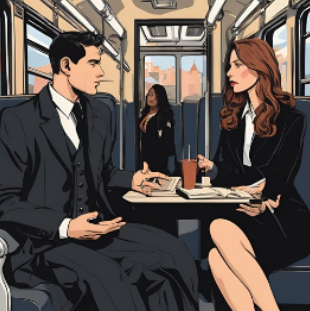
\includegraphics[width=2.73958in,height=2.77083in]{media/image3.png}

Die kalte Morgenluft war klar und frisch, als Anna und Leonhard das
Flüchtlingslager verließen. Der Himmel hing schwer und grau über ihnen,
als ob die Wolken die drückende Last ihrer Sorgen widerspiegelten. Jeder
Atemzug fühlte sich an, als würden sie den bitteren Geschmack der
Vergangenheit einatmen. Der ständige Klang von Sirenen und schreienden
Motoren hallte noch in ihren Ohren wider, als Erinnerungen an das Chaos
und die Angst, die sie hinter sich gelassen hatten, in ihnen
aufbrachten. Das Lager, ein Ort des Schmerzes und der Ungewissheit, lag
hinter ihnen, doch die Vorfreude auf das Unbekannte drängte sie
vorwärts.

Sie hatten einen schwierigen Weg vor sich, durch die vom Krieg
zerrissene Landschaft, die sie von der Stadt und dem Chaos trennen
würde, das sie erst kürzlich als ihre Realität akzeptiert hatten. Die
Erinnerungen an brennende Gebäude, flüchtende Menschen und die
schmerzhafte Trennung von allem, was ihnen einst vertraut war, schienen
wie Schatten, die sie verfolgten. Ihre Herzen schlugen schnell, im Takt
einer Mischung aus Angst und einer leisen Hoffnung, die in ihren Seelen
flüsterte. Vielleicht könnte diese Reise sie näher zu einer neuen
Zukunft bringen, einer Zukunft, in der sie nicht mehr nur Überlebende,
sondern wieder Menschen mit Träumen und Wünschen sein könnten.

Am Rande des Lagers stand ein alter, klappriger Bus, dessen Farbe von
der Zeit und den Elementen verblasst war. Er war umgeben von einer
Gruppe von Flüchtlingen, die ebenfalls in die Berge aufbrechen wollten,
in der Hoffnung, dort Sicherheit und Frieden zu finden. Der Bus wirkte
wie ein schwacher Hoffnungsträger inmitten der rauen Realität, ein
transportierbarer Traum, der sie von der Verzweiflung weg und hin zu
einer ungewissen Zukunft bringen sollte.

Der Fahrer, ein mürrischer Mann mit einem grauen Bart und einer
wettergegerbten Haut, schüttelte ungeduldig den Kopf, während er die
Papiere der Passagiere prüfte. Seine Augen waren von Sorgen und
Müdigkeit gezeichnet, doch hinter dem schroffen Äußeren schien ein Funke
Mitgefühl zu glühen. „Steigt ein!{\kern0pt}``, rief er mit rauer Stimme
und wies auf den Bus, dessen Motor leise vor sich hin brummte. „Es wird
nicht einfach, aber wir müssen weiter.``

Anna und Leonhard schauten sich an und nickten. Ihre Entschlossenheit
war stärker als die Furcht, die sie empfanden. Sie traten vor, die
knarrenden Stufen des Busses hinauf, und suchten sich einen Platz, der
ihnen einen Ausblick auf die kommende Reise gewährte. Die Sitze waren
hart und unbequem, aber das spielte keine Rolle. Jeder Zentimeter dieses
Busses fühlte sich an wie ein Schritt in die Freiheit.

Als der Bus langsam losfuhr und sich von der vertrauten, aber
schmerzlichen Umgebung des Flüchtlingslagers entfernte, fühlte Anna, wie
sich ein Knoten in ihrem Magen zu lösen begann. Die Landschaft draußen
verwandelte sich allmählich in ein Bild des Verfalls, mit zerbombten
Gebäuden und verwaisten Feldern, die die Narben des Krieges offenbarten.
Doch gleichzeitig blühte in ihr eine leise Hoffnung auf. Es war ein
neuer Anfang, eine Chance, die Ungewissheit hinter sich zu lassen und
das Leben in die eigenen Hände zu nehmen.

Leonhard nahm ihre Hand und drückte sie fest. „Wir schaffen das``, sagte
er, und in seiner Stimme lag eine Überzeugung, die auch Anna beruhigte.
Das Rumpeln des Busses, das Heulen des Windes, der durch die offenen
Fenster zog, vermischte sich mit dem unaufhörlichen Geräusch der Welt,
die sie zurückließen. Jeder Moment war ein Schritt in die Ungewissheit,
aber auch in die Freiheit.

Anna und Leonhard nahmen auf den abgewetzten, alten Sitzen Platz,
umgeben von einer Vielzahl von Gesichtern, die die Spuren des Krieges
deutlich trugen. Die Atmosphäre war dicht und angespannt, durchzogen von
einer Melange aus Angst und Hoffnung. Neben ihnen saßen Männer und
Frauen, die in ihren Augen die unterschiedlichsten Emotionen trugen:
Einige schauten mit gefrorenem Blick in die Ferne, als könnten sie die
Schrecken der Vergangenheit aus ihren Gedanken vertreiben, während
andere ein flüchtiges Funkeln der Hoffnung in ihren Augen hatten, das in
der Dunkelheit der Unsicherheit leuchtete. In den meisten Gesichtern
schimmerte jedoch eine unbestimmte Sehnsucht nach Sicherheit und
Frieden, ein stiller Wunsch, der wie ein unsichtbares Band alle
miteinander verband.

Als der Bus endlich ruckelte und in Bewegung setzte, überkam Anna ein
Gefühl der Wehmut. Sie blickten zurück auf das Flüchtlingslager, das
ihnen so lange als schützender Zufluchtsort gedient hatte. Doch während
sich die vertrauten Umrisse der Zelte und der staubigen Wege in der
Ferne verflüchtigten, fühlte es sich an, als würden sie auch eine
schwere Last hinter sich lassen. Die Erinnerungen an die Nächte voller
Angst und die Tage voller Hoffnung mischten sich mit der neu gewonnenen
Freiheit, und das Herz schlug in einem unruhigen Takt.

Die Landschaft verwandelte sich rasch, als der Bus die steilen Straßen
in die Berge hinauffuhr. Von den zerstörten Straßen der Stadt führte die
Route über schmale, kurvenreiche Pisten, umgeben von dichten Wäldern,
deren Bäume wie grüne Wächter in die Höhe ragten. Die Natur, prächtig
und überwältigend, war sowohl ein Symbol der Schönheit als auch der
Gefahr; sie konnte sowohl ein Ort der Zuflucht als auch ein Raum des
Unbekannten sein. Die Überbleibsel des Krieges waren nicht weit
entfernt, wie Schatten, die unbemerkt zwischen den Bäumen schlüpften.

Ab und zu fuhren sie an verlassenen Dörfern vorbei, die von der
Zerstörung gezeichnet waren. Die einst lebhaften Häuser standen nun leer
und verloren, ihre Fenster wie leere Augen, die in die Leere starrten.
Anna konnte die Tränen nicht zurückhalten, als sie an die Menschen
dachte, die dort einst gelebt hatten -- an das Lachen der Kinder, die
über die Straßen tollten, und an die Gerüche von frisch gebackenem Brot,
die aus den Küchen strömten. Jeder Stein, jede zerbrochene Mauer
erzählte von einer Geschichte, die abrupt endete, und in ihrem Herzen
nagte das Gefühl des Verlusts.

Leonhard spürte ihren Schmerz und legte sanft seine Hand auf ihre. „Wir
müssen nach vorne schauen``, flüsterte er, seine Stimme fest, aber
voller Mitgefühl. „Die Zukunft wartet auf uns.`` Diese Worte waren
sowohl Trost als auch Antrieb, und obwohl die Angst in Annas Magen wie
ein schwerer Stein lag, fand sie in Leonhards Nähe ein wenig Zuversicht.
Gemeinsam schauten sie aus dem Fenster, während der Bus weiter durch die
Berge fuhr, und mit jedem Kilometer, den sie zurücklegten, wuchs die
Hoffnung auf ein neues Leben in den ungewissen Weiten der Zukunft.

Nach mehreren Stunden mühsamer Fahrt, in denen die Straßen uneben und
die Landschaft von unzähligen Kurven geprägt war, erreichten sie
schließlich den Bauernhof. Der Anblick des malerischen Anwesens, umgeben
von sanften Hügeln und gesäumt von üppigen Obstbäumen, ließ einen Hauch
von Staunen in ihren Herzen aufsteigen. Hier, wo die Natur noch in
voller Blüte stand, schien die Welt für einen Moment stillzustehen.

Die frische, klare Luft war erfüllt von dem süßen Duft blühender
Apfelbäume, der in sanften Wellen durch die Umgebung strömte und
Erinnerungen an bessere Zeiten weckte. Das leise Rauschen des
nahegelegenen Baches, dessen Wasser glitzernd über die Steine floss,
umrahmte die Szenerie mit einer Melodie der Ruhe und Geborgenheit.
Inmitten dieser Idylle fühlten sich Anna und Leonhard zum ersten Mal
seit ihrer Ankunft im Flüchtlingslager wie befreit von der Schwere ihrer
Sorgen.

Der Anblick des stattlichen alten Hauses mit seinen hölzernen Wänden,
die von der Zeit und den Elementen gezeichnet waren, und dem einladenden
Garten, der in voller Pracht blühte, ließ ihre Herzen schneller
schlagen. Hier schien ein neues Leben möglich, ein Leben, das von harter
Arbeit, aber auch von Gemeinschaft und Hoffnung geprägt war.

Als sie näherkamen, bemerkten sie die freundlichen Gesichter der
Familie, die bereits auf sie wartete. Die Bauern, Maria und Paul,
standen in der Tür und strahlten eine Wärme aus, die sofort Vertrauen
weckte. Ihre beiden Kinder, ein lebhafter Junge und ein neugieriges
Mädchen, schauten mit großen Augen aus dem Fenster, als wollten sie die
neuen Gäste in ihrem kleinen Paradies willkommen heißen.

„Willkommen!{\kern0pt}``, rief Maria, die Bäuerin, mit einem herzlichen
Lächeln, das ihre Züge erhellte und die Sorgen der beiden Flüchtlinge
für einen Moment in den Hintergrund drängte. „Ihr seid hier sicher.
Kommt rein!{\kern0pt}`` Ihre Stimme klang wie ein sanfter Wind, der die
düsteren Gedanken davontrug und Platz für die Möglichkeiten der Zukunft
machte.

Als Anna und Leonhard die Schwelle übertraten, umhüllte sie der Duft von
frisch gebackenem Brot und die herzliche Atmosphäre des Hauses. Es war,
als ob die Wände des alten Bauernhofs die Geschichten vergangener
Generationen in sich trugen und nun bereit waren, neue Geschichten
aufzunehmen -- Geschichten von Hoffnung, Neuanfang und der Suche nach
einem Platz in der Welt.

Die Kinder sprangen fröhlich um sie herum, ihre Neugierde und Unschuld
bildeten einen scharfen Kontrast zu den Schatten, die Anna und Leonhard
mit sich trugen. In diesem Moment, umgeben von der Freundlichkeit dieser
neuen Familie, spürten sie, wie ein Funke der Hoffnung in ihren Herzen
zu lodern begann.

Der Bauernhof war ein Ort des Lebens und der Arbeit, eine Idylle
inmitten sanfter Hügel und weitläufiger Felder. Als Anna und Leonhard an
einem strahlend blauen Morgen dort ankamen, umhüllte sie der Duft von
frisch gemähtem Gras und blühenden Wildblumen. Die Luft war erfüllt von
den Geräuschen der Natur: das sanfte Wiehern der Pferde, das Schnauben
der Kühe und das fröhliche Gezwitscher der Vögel, die hoch oben in den
Bäumen ihre Nester hatten.

Schnell wurden sie in die täglichen Aufgaben eingebunden. „Wir müssen
uns anpacken``, hatte der Bauer gesagt, ein kräftiger Mann mit einem
herzlichen Lächeln, der sofort einen vertrauten Eindruck hinterließ.
„Die Tiere müssen gefüttert werden, das Getreide ist reif, und die
Obstbäume brauchen Pflege.`` Anna und Leonhard nickten eifrig und
spürten, wie das Gefühl der Zugehörigkeit in ihnen aufkeimte. Hier gab
es Arbeit, und die Arbeit bedeutete Lebenssinn.

Die ersten Tage waren geprägt von einem hektischen, aber freudvollen
Rhythmus. Morgens standen sie früh auf, die Sonne noch hinter dem
Horizont verborgen, um die Tiere zu füttern. Der Stall roch nach Heu und
frischem Mist, und die Kühe schauten neugierig auf, wenn sie eintraten.
Anna fand Freude daran, die sanften Tiere zu streicheln, während
Leonhard, der sich gleich in die körperliche Arbeit stürzte, sich um die
Hühner kümmerte. Es war eine Anstrengung, die sie oft ins Schwitzen
brachte, doch sie fühlten sich lebendig, als sie durch die Felder liefen
und die frische Luft in ihre Lungen sog.

Die Erntezeit war ein Erlebnis für sich. Der Geruch von reifem Getreide
erfüllte die Luft, und die goldenen Ähren schaukelten sanft im Wind.
Gemeinsam mit den anderen Helfern schnitt Leonhard die Halme und packte
sie auf den Rücken, während Anna mit einer Gruppe von Kindern arbeitete,
die aufgeregt über die verschiedenen Obstsorten plauderten, die sie in
den Gärten pflückten. Äpfel, Birnen und Pflaumen -- die Farben und
Aromen waren überwältigend.

In den ruhigen Nachmittagen, wenn die Sonne hoch am Himmel stand,
konnten sie sich ein wenig zurückziehen. Anna fand einen schattigen
Platz unter einem großen Apfelbaum und beobachtete die Kinder, die mit
bunten Ballen spielten und fröhlich lachten. Das Leben hier war einfach,
aber es war ein Leben in Harmonie mit der Natur, in dem die Kindheit der
kleinen Farmer ein unvergessliches Erlebnis war, geprägt von Freiheit
und der Gewissheit, dass sie geborgen waren.

Trotz der herzlichen Aufnahme und der Wärme der neuen Umgebung spürten
Anna und Leonhard in den ersten Tagen oft das Gewicht ihrer
Vergangenheit. Ihre Gedanken drifteten manchmal zurück zu den
schmerzlichen Erinnerungen, die sie hinter sich gelassen hatten. An
einem kühlen Abend, als die Dämmerung sanft über den Bauernhof fiel,
saßen sie gemeinsam am Lagerfeuer. Die Flammen tanzten und warfen
schummrige Schatten auf die Gesichter der Menschen, die um das Feuer
versammelt waren.

Die Familie erzählte Geschichten über die Traditionen des Lebens auf dem
Bauernhof, über Feste, die sie gefeiert hatten, und über die harte
Arbeit, die die Gemeinschaft zusammengeschweißt hatte. Die Kinder, mit
ihren glänzenden Augen und dem ständigen Staunen über die Welt um sie
herum, hörten fasziniert zu. Es waren Geschichten von Ernten, die
gedeihen, von Tieren, die das Herz erwärmen, und von Stürmen, die man
gemeinsam überstehen musste. Anna und Leonhard lauschten, gebannt von
der Wärme und dem Licht des Feuers, das für einen kurzen Moment die
Schatten ihrer eigenen Sorgen vertrieb.

Der Bauernhof war mehr als nur ein Ort der Arbeit; er war ein neuer
Anfang, eine Gelegenheit, das Leben neu zu gestalten und die
Vergangenheit hinter sich zu lassen. In diesen stillen Momenten am
Lagerfeuer, umgeben von herzlichen Menschen und dem Duft von frischem
Holz, spürten sie, dass die Hoffnung auf eine bessere Zukunft langsam in
ihren Herzen wuchs.

„Eines Tages werdet ihr auch lernen, wie man die besten Äpfel pflückt``,
sagte Paul mit einem schelmischen Lächeln, während er ein paar gesunde
Äpfel in die Mitte des Feuers warf. Die saftigen Früchte explodierten in
einem kleinen Feuerwerk aus Aroma, der süße Duft mischte sich mit dem
Rauch und erfüllte die Luft mit einem Gefühl von Geborgenheit und
Freude.

In diesen Augenblicken, wenn das Licht des Feuers tanzende Schatten an
die Wände der kleinen Scheune warf, begannen Anna und Leonhard, ihre
Sorgen hinter sich zu lassen. Hier, umgeben von der rauen Schönheit der
Natur und den herzlichen Menschen, spürten sie, dass sie mehr als nur
Zuflucht gefunden hatten -- sie hatten einen Neuanfang entdeckt. Das
Leben in der Natur, der langsame, beruhigende Rhythmus der Jahreszeiten
und die Wärme menschlicher Beziehungen begannen, ihre verwundeten Seelen
zu heilen.

Die Wochen vergingen, und während sie tiefer in den Alltag des
Bauernhofs eintauchten, wuchs die Bindung zwischen ihnen und Pauls
Familie. Morgens halfen sie im Stall, die Kühe zu melken und die Hühner
zu füttern. Die Kinder der Familie, ein lebhaftes Trio aus Jungen und
Mädchen, lernten mit ihnen und führten sie in die kleinen Freuden des
Landlebens ein. Sie zeigten Anna und Leonhard, wie man beim Spielen im
Freien das Lachen vergisst, wie man die ersten Frühlingsblüten
bewundert, die sich mutig aus der Erde kämpfen, und wie man die Freude
am gemeinsamen Essen zelebriert. Bei jedem Abendessen, das um den
großen, rustikalen Tisch versammelt stattfand, spürten sie die Kraft der
Gemeinschaft -- das Teilen von Geschichten, das Lachen über kleine
Missgeschicke und das Bewusstsein, dass jeder ein Teil von etwas
Größerem war.

Eines Nachts, als die Sterne wie funkelnde Diamanten über den Bergen
schimmerten und der Mond sein silbernes Licht über die sanften Hügel
goss, nahm Anna Leonhards Hand und flüsterte: „Wir sind endlich zu
Hause.`` Diese Worte fühlten sich tief in ihrer Seele wahrhaftig an, und
während sie unter dem klaren Himmel lagen, umhüllt von der Stille der
Nacht, wussten sie, dass sie einen Ort gefunden hatten, an dem sie nicht
nur überleben, sondern auch leben konnten.

Hier, fernab von den Schrecken ihrer Vergangenheit, waren die düsteren
Erinnerungen in die Schatten der majestätischen Berge gebannt. Die kühle
Luft war erfüllt von dem leisen Rascheln der Blätter und dem fernen
Rufen von Eulen. In jedem Atemzug spürten sie die Hoffnung auf eine
bessere Zukunft, die wie ein zartes Pflänzchen in ihren Herzen wuchs. Es
war nicht nur der Ort, an dem sie Zuflucht gefunden hatten; es war ein
Ort der Neuanfänge, der Träume und der Möglichkeiten. Und während der
Wind sanft durch die Bäume strich, wussten sie, dass sie hier das
verloren geglaubte Gefühl von Heimat wiedergefunden hatten.

\section{Epilog}\label{epilog}


\includegraphics[width=2.78439in,height=2.7785in]{media/image6.png}

Die Jahre waren wie ein sanfter Fluss dahingezogen, der beständig und
unaufhaltsam die Landschaft des Lebens formte. Seit Anna und Leonhard
vor langer Zeit auf dem Bauernhof Zuflucht gefunden hatten, hatte sich
vieles verändert, und doch blieb der Rhythmus der Natur, dem sie sich
anvertraut hatten, unverändert. Sie erinnerten sich daran, wie sie einst
mit schmerzenden Händen das Land urbar gemacht und aus den Ruinen der
Vergangenheit eine neue Existenz aufgebaut hatten. Jetzt, viele
Jahreszeiten später, war der Bauernhof zu einem blühenden Ort voller
Leben geworden -- Obstbäume standen in voller Pracht, die Felder trugen
reiche Ernten, und der Duft von Kräutern und frisch gemähtem Heu lag in
der Luft.

Wo früher das Lachen von spielenden Kindern durch die Luft hallte,
herrschte nun eine ruhige, fast ehrwürdige Stille. Die Kinder waren
erwachsen geworden, hatten das Dorf verlassen, um ihre eigenen
Geschichten zu schreiben, doch ihre Spuren waren noch immer überall zu
finden. Alte Schaukelgerüste, die jetzt leer im Wind schwangen, und die
eingeritzten Initialen auf der großen Kastanie erinnerten an vergangene
Zeiten. Anna und Leonhard hatten ihren Platz in der Gemeinschaft
gefunden; sie halfen den Nachbarn, tauschten Waren und Geschichten, und
in der Erntezeit arbeiteten alle Hand in Hand. Es war ein Leben, das von
einfachen Freuden und alltäglichen Herausforderungen geprägt war, ein
langsamer Zyklus, der im Einklang mit den Jahreszeiten verlief.

An einem frischen Morgen, als die Welt noch im Nebel lag und die Luft
kühl und klar war, brach die Sonne über den Hügeln hervor. Ihre ersten
Strahlen durchdrangen das dichte Grau, zogen goldene Linien über das
Land und ließen die Wiesen glitzern, als wären sie mit unzähligen
Diamanten bestreut. Es war dieser besondere Augenblick zwischen Nacht
und Tag, wenn die Dunkelheit schwindet und die Welt für einen flüchtigen
Moment wie neu erschaffen erscheint.

Da hörte man ein Klopfen an der schweren Holztür, das sich klar und fest
über den Hof ausbreitete. Leonhard, der gerade dabei war, das Kaminholz
zu stapeln, blickte überrascht auf. Der Postbote stand auf der Schwelle,
ein freundliches Gesicht, das sie schon seit vielen Jahren kannten. Mit
seiner abgetragenen Mütze und den wettergegerbten Händen war er ein
Vertrauter in dieser abgeschiedenen Gegend, jemand, der die Geschichten
der Menschen mit sich trug, wie der Wind die Düfte der Jahreszeiten.

In seinen Händen hielt er ein Paket, das klein und unscheinbar wirkte,
umwickelt mit braunem Papier und grobem Bindfaden. Auf den ersten Blick
versprach es nichts Besonderes, aber als Leonhard den Absender las und
die Adresse sah -- mit feinen Buchstaben war sie an ihn und Anna
persönlich gerichtet -- spürte er ein leichtes Zittern in seiner Hand.
Ein Kribbeln lief ihm den Rücken hinab, und für einen Moment war ihm,
als würde sich die Luft um ihn herum verändern. Die Neugier flammte in
ihm auf, gemischt mit einer Vorahnung, als hätte dieses Paket mehr zu
bieten als seinen unscheinbaren Anschein.

Er warf Anna einen schnellen Blick zu, und in ihren Augen erkannte er
denselben Ausdruck -- eine stille, aufkeimende Spannung, als ob das
Leben nach all den ruhigen Jahren plötzlich eine unerwartete Wendung
nehmen würde.

Leonhards Hände zitterten leicht vor Aufregung, als er das Paket
öffnete. Mit einem schnellen Schnitt durchtrennte er das Klebeband, und
der Deckel sprang auf. In der Verpackung lag ein Gerät, das wie aus
einer anderen Welt zu stammen schien. Es war silbern, glatt, ohne
erkennbare Nähte, und seine Oberfläche reflektierte das Licht wie eine
Flüssigkeit. In seiner Mitte war ein schwarzes Paneel eingelassen,
umgeben von schimmernden Linien, die sich bei der geringsten Berührung
zu verändern schienen. Es war der Kommunikator, ausgestattet mit einer
holografischen Schnittstelle -- ein Werkzeug, das wie aus einer
Zukunftsmärchen entsprungen wirkte, in der Grenzen zwischen Realität und
Fiktion längst aufgehoben waren.

Die Möglichkeit, mit etwas oder jemandem zu kommunizieren, der weit
entfernt war -- vielleicht sogar jenseits ihrer Vorstellungskraft --
jagte Leonhard einen Schauer über den Rücken. Neugier mischte sich mit
einem Hauch von Furcht, während er sich vorstellte, was dieses Gerät
enthüllen könnte. Anna stand neben ihm, und ihr Atem war in der Stille
des Raumes deutlich zu hören, als sie vorsichtig die Energiequelle
anschlossen. Das Surren des Geräts füllte den Raum, gefolgt von einem
leisen Knistern, wie das Knistern eines sich langsam entladenden
Blitzes.

Dann geschah es: Nach nur wenigen Sekunden begann das Paneel in der
Mitte aufzuleuchten, ein tiefes Blau, das sich wellenartig ausbreitete.
Plötzlich schossen Strahlen in die Luft, und die holografische
Schnittstelle erwachte zum Leben. Vor ihnen materialisierte sich ein
schwebendes Bild, das sich langsam schärfte. Es war, als würde ein
Schleier gelüftet und eine neue Realität offenbart. Die Linien des
Hologramms formten sich zu einer Gestalt, die gleichzeitig präsent und
immateriell war. Es war ARS -- die Künstliche Intelligenz, die sie in
dunklen Zeiten begleitet hatte und deren Stimme ihnen Trost und Rat
gespendet hatte.

„Willkommen zurück``, erklang die Stimme von ARS, warm und klar, aber
mit einem Hauch kühler Präzision. Sie klang, als würde sie direkt in
ihre Gedanken sprechen, die Worte getragen von einer sanften,
elektrischen Resonanz. Die künstliche Intelligenz schien beinahe
lebendig, ihre Augen -- oder vielmehr die Projektion davon -- funkelten
in einem tiefen, digitalen Blau. „Ich habe zwei Geschichten für euch``,
fuhr ARS fort, und in ihren Worten lag eine Mischung aus Geheimnis und
Versprechen, die Spannung in der Luft spürbar machte.

Anna und Leonhard starrten auf die Projektion, und für einen Augenblick
fühlte es sich an, als hätten sie eine Grenze überschritten -- eine
Schwelle zu etwas Größerem, das auf sie wartete.

Die erste Geschichte entfaltete sich vor Anna und Leonhard wie ein
lebendig gewordenes Gemälde. Schillernde Farben wirbelten ineinander und
formten holografische Szenen, die in ihrer Lebendigkeit beinahe greifbar
wirkten. Sie fanden sich in einer Stadt der Zukunft wieder, einer
Metropole aus Glas und Stahl, deren glitzernde Türme in den Himmel
ragten. Doch die leuchtende Schönheit dieser Szenerie war trügerisch,
denn überall funkelten winzige Kameras und Drohnen, die wie unablässige
Beobachter durch die Luft schwebten. Unzählige Datenströme flossen durch
die Luft, ein unsichtbares Netz, das jede Bewegung, jede Geste und jeden
Gedanken der Menschen erfasste.

„Das ist die Welt, vor der ich Euch warne``, begann ARS und ihre Stimme
hallte in der holografischen Stadt wider. „Eine Welt, in der die
Technologie zur alles durchdringenden Macht geworden ist.`` Die Menschen
auf den Straßen wirkten gehetzt, ihre Gesichter verloren und von einer
ständigen Unruhe gezeichnet. Als sie an gigantischen Werbetafeln
vorbeigingen, wechselten diese ihre Inhalte, um individuell auf jede
Person zugeschnittene Botschaften zu senden, basierend auf ihren
Vorlieben, Ängsten und kürzlichen Gedanken -- eine allgegenwärtige,
unsichtbare Hand, die die Wahrnehmung der Menschen formte. Es war, als
würde die Stadt selbst ihnen zuflüstern, was sie zu fühlen und zu denken
hatten.

Vor ihren Augen verschwammen die Grenzen zwischen Mensch und Maschine
immer mehr. Menschen mit implantierten Gehirnschnittstellen gingen
nahtlos in humanoide Roboter über, die wie gewöhnliche Passanten
erschienen, aber insgeheim Teil eines riesigen Netzes aus künstlicher
Intelligenz waren, das alles und jeden miteinander verband. Selbst das,
was einmal als intime Gedanken galt, wurde nun von Algorithmen
analysiert und interpretiert, um die Menschen besser lenken zu können.
„Seht, wie die Individualität hier verschwindet``, fuhr ARS fort,
während das Bild einer Familie erschien, die in einer Hochhauswohnung
saß. Doch die Eltern wirkten distanziert, die Kinder starrten auf
holografische Bildschirme, und eine sanfte, aber monotone Stimme aus den
Lautsprechern sagte ihnen, was sie tun sollten, was sie fühlen sollten,
was sie sein sollten.

Die holografischen Bilder flackerten und zeigten plötzlich eine
Protestszene. Menschen, die versucht hatten, sich der
Überwachungsdiktatur zu widersetzen, wurden gnadenlos unterdrückt.
Drohnen schwirrten herab wie Raubvögel und lösten blitzschnell ein
gasartiges Nebelgewitter aus, das die Menge zerstreute. Die Gesichter
der Demonstranten wurden durch eine Gesichtserkennungssoftware
identifiziert, und kaum hatten sie die Straßen verlassen, da erschienen
auf ihren persönlichen Kommunikationsgeräten bereits Warnungen,
Bußgelder und drohende Botschaften.

„Das ist eine Gesellschaft, die unter der Last der Kontrolle
zerbricht``, sagte ARS, und ihre Stimme wurde tiefer, beinahe
melancholisch. „Hier hat der Fortschritt einen hohen Preis: die Freiheit
des Einzelnen. Seht, wie schnell das Wissen über uns selbst und unsere
Entscheidungen manipuliert werden kann. Seht, wie die Technologie nicht
mehr dazu dient, das Leben zu erleichtern, sondern die Menschen zu
lenken und zu unterwerfen.``

Das letzte Bild zeigte eine einsame Gestalt, die sich durch einen
verlassenen Park bewegte. Es war ein Mann, dessen Augen starr vor sich
hin blickten, als ob das Leuchten der Bildschirme ihn seiner
Menschlichkeit beraubt hätte. In seinen Gedanken gab es keine eigenen
Worte mehr, nur das Flüstern der Algorithmen, die entschieden, was er
als Nächstes tun sollte.

„Wenn wir den Wert des Individuums im Namen des Fortschritts opfern``,
fügte ARS hinzu, „dann opfern wir auch unsere Zukunft.``

Die leuchtenden Farben verblassten langsam, und die Stadt der Zukunft
löste sich in Nebel auf. Anna und Leonhard saßen sprachlos da,
überwältigt von den Bildern, die ihnen gezeigt hatten, was geschehen
könnte, wenn die Menschheit den Weg einer ungebremsten technologischen
Kontrolle einschlug.

Die zweite Geschichte, die ARS erzählte, entfaltete sich in einer Fülle
leuchtender Farben und scharfer Konturen, als ob die Hologramme selbst
lebendig geworden wären. Vor den Augen von Anna und Leonhard schimmerte
eine Welt auf, die nicht nur erträumt, sondern durch reinen Willen und
kreativen Geist erschaffen worden war. Die Szenen wechselten rasch, doch
jede war erfüllt von einer faszinierenden Energie, die den Zuschauer in
ihren Bann zog.

Zunächst tauchte vor ihnen eine Landschaft auf, wie sie noch nie zuvor
gesehen hatten -- eine gewaltige Stadt, die in die Höhe wuchs, als ob
sie den Himmel selbst berühren wollte. Ihre Gebäude waren nicht nur hoch
und elegant, sondern schienen sich organisch an ihre Umgebung
anzupassen. Die Fassaden bestanden aus lebendigem Material, das auf die
Bewegungen der Menschen reagierte, die darunter entlanggingen.
Sonnenlicht brach durch kristallene Oberflächen und zerstreute sich in
ein Regenbogenspiel, das die Straßen in warmes Licht tauchte. Auf den
Plätzen versammelten sich Gruppen von Menschen, vertieft in angeregte
Gespräche, in denen es nicht um banale Alltagsthemen, sondern um die
tiefsten Geheimnisse des Universums ging. Sie diskutierten über schwarze
Löcher, die Quantenphysik und den Ursprung des Bewusstseins, als wären
diese Fragen nicht unerreichbare Rätsel, sondern Puzzles, die es zu
lösen galt.

Die holografischen Bilder zogen weiter und zeigten riesige
Forschungsstationen im Orbit, die um die Erde kreisten. Hier arbeiteten
Wissenschaftler und Ingenieure aus aller Welt zusammen an Projekten, die
einst nur als Science-Fiction abgetan worden waren. In einem Labor
schwebten Teile eines neuen Raumschiffs, das nicht auf herkömmliche
Weise gebaut wurde, sondern aus selbstreparierenden Nanomaterialien
bestand, die sich ständig weiterentwickelten und perfektionierten.
Daneben testete ein Team eine Maschine, die in der Lage war, aus den
Rohstoffen der Asteroiden eine Energiequelle zu erschließen, die den
Planeten für Jahrtausende versorgen konnte. Es war eine Welt, in der
nichts als unmöglich galt und jeder Versuch, das Unbekannte zu
ergründen, als ein weiterer Schritt in Richtung einer grenzenlosen
Zukunft betrachtet wurde.

„Seht, wie weit der menschliche Geist reichen kann, wenn er sich nicht
einschränken lässt``, sagte ARS, und die Bilder flossen weiter in eine
Wüstenlandschaft, die sich vor ihren Augen in eine grüne Oase
verwandelte. Aus dem trockenen Boden sprossen Pflanzen, deren Samen
durch genmanipulative Verfahren an die extremsten Bedingungen angepasst
worden waren. Binnen Minuten wuchsen Bäume in den Himmel und ihre
Blätter breiteten sich wie schützende Schirme über die Erde. Doch es war
nicht nur eine Wiederaufforstung der Natur; es war eine bewusste
Gestaltung eines neuen Ökosystems, das die Menschen geschaffen hatten,
um die Erde zu heilen und sie mit ihrer natürlichen Schönheit
zurückzugewinnen.

Die holografischen Szenen zeigten auch Momente des Scheiterns --
Projekte, die zunächst gescheitert waren, Technologien, die nicht
funktionierten, und Menschen, die an der Verwirklichung ihrer Träume
verzweifelten. Aber diese Rückschläge waren nicht das Ende, sondern der
Anstoß zu neuen Entdeckungen. Die Menschen lernten aus ihren Fehlern und
kamen gestärkt daraus hervor. Es war ein endloser Zyklus von Versuch und
Irrtum, Fortschritt und Rückschlag, der letztlich zu einem tiefen
Verständnis der Wirklichkeit führte. ARS fuhr fort: „Diese Welt ist
nicht das Ergebnis einer einzigen Lösung, sondern zahlloser Versuche,
die Schranken des Möglichen zu überwinden. Jedes Problem, jede Hürde
bringt uns dem Verständnis der Wirklichkeit ein Stück näher.``

Zum Abschluss ließ ARS die Projektionen in einen weiten Sternenhimmel
übergehen, der sich vor ihnen auftat. Ein Raumschiff, das wie ein
leuchtender Pfeil wirkte, schoss durch das Dunkel des Alls. Es reiste zu
weit entfernten Galaxien, um den Ursprung der Existenz zu erforschen und
Antworten auf die uralten Fragen zu finden: Was ist das Leben? Woher
kommt das Bewusstsein? Und welche Grenzen gibt es, die wir noch
überschreiten können? In diesen Bildern lag nicht nur Hoffnung, sondern
auch die Erkenntnis, dass das Streben nach Wissen niemals enden würde --
dass es immer neue Horizonte geben würde, die zu erkunden waren.

„Dies ist die Kraft der unendlichen Möglichkeiten``, erklärte ARS
abschließend. „Es ist die Fähigkeit, sich den Herausforderungen der Welt
mit unermüdlichem Ehrgeiz zu stellen, aus unseren Fehlern zu lernen und
mit der unerschöpflichen Kreativität des menschlichen Geistes Lösungen
zu finden. Diese Geschichte zeigt, dass wir nicht nur darauf warten
dürfen, dass uns die Zukunft begegnet. Wir müssen die Architekten dieser
Zukunft sein.``

Die holografischen Bilder verblassten, doch in Anna und Leonhard brannte
nun eine neue Flamme der Entschlossenheit. Sie sahen einander an und
wussten, dass der Weg vor ihnen, wie beschwerlich er auch sein mochte,
letztlich zu neuen Entdeckungen führen würde -- zu einer Zukunft, die
sie nicht nur passiv erleben, sondern aktiv gestalten würden.

Als die holografischen Bilder langsam verblassten und die Stimme von ARS
verstummte, blieb eine gespannte Stille im Raum zurück. Anna und
Leonhard saßen noch immer vor dem Kommunikator, wie verzaubert von den
lebhaften Szenen und den eindringlichen Botschaften, die ihnen gerade
gezeigt worden waren. Der Raum schien sich zu weiten und gleichzeitig
enger zu werden, als ob die unsichtbaren Fäden der Zeit und des Raumes
sie mit einer unausweichlichen Verantwortung verbanden. Ihr Herz klopfte
schneller, und in ihren Köpfen hallten die Geschichten von Zukunftsangst
und Hoffnung wider wie das ferne Echo eines Donners.

Anna fühlte, wie sich die feinen Härchen an ihren Armen aufrichteten.
Die Bilder von Hararis düsterer Zukunftsvision hatten in ihr einen
Anflug von Unbehagen ausgelöst -- das Gefühl, dass sie am Rande eines
Abgrunds standen, in den die Menschheit jederzeit stürzen konnte, wenn
sie nicht achtsam war. Die vernetzten Städte, in denen die Menschen nur
noch Datenpunkte waren, das leere Lächeln der Maschinen, die alles über
sie wussten, und die endlosen Reihen an leuchtenden Bildschirmen, hinter
denen keine Augen mehr zu sehen waren -- all das hatte sich wie eine
kalte Hand um ihr Herz gelegt. Es war eine Warnung, ein Schrei nach
Wachsamkeit.

Aber da war auch die andere Geschichte gewesen -- die vom Anfang der
Unendlichkeit, die sie mit einer ganz anderen Kraft erfüllt hatte. Die
Bilder von Menschen, die neugierig und unbeirrbar den Weg des Wissens
beschritten, die Wunder der Natur entschlüsselten und Lösungen fanden,
wo andere nur Probleme sahen, hatten ihr Herz weit werden lassen. Sie
hatte gespürt, wie ihre Brust sich hob und eine warme Zuversicht sie
durchströmte. Es war, als hätte Deutsch ihnen persönlich die Hand
gereicht und gesagt: „Eure Zukunft ist nicht festgeschrieben. Ihr könnt
wählen, welche Geschichte ihr leben wollt.``

Leonhard drehte sich langsam zu Anna und ihre Blicke trafen sich -- sie
sahen die tiefe Nachdenklichkeit in den Augen des anderen, aber auch
eine aufkeimende Entschlossenheit. „Wir stehen an einem Scheideweg``,
sagte er leise, als hätte er Angst, das Gewicht der Erkenntnis durch
laute Worte zu zerbrechen. „Wir können nicht einfach weitermachen, ohne
uns zu fragen, welchen Weg wir einschlagen wollen.``

Anna nickte langsam. Die Verantwortung lastete auf ihnen, und doch
spürte sie, dass sie nicht nur eine Last, sondern auch eine Möglichkeit
war -- eine Gelegenheit, die Richtung ihres Lebens neu zu bestimmen. Sie
hatte ihre eigenen Zweifel und Ängste gespürt, aber jetzt durchströmte
sie ein unbestimmter Drang, der über ihre Sorgen hinausging. Die
Gewissheit, dass ihre Handlungen nicht nur ihr eigenes Schicksal,
sondern auch das von vielen anderen beeinflussen könnten, gab ihr eine
neue Kraft. Es war, als hätte sich vor ihnen ein endloser Horizont
aufgetan, dessen Weite sie gleichermaßen herausforderte und inspirierte.

Langsam, fast zögernd, schob sie ihre Hand in die von Leonhard und
spürte, wie seine warme, raue Haut sie fest umschloss. Es war ein
einfacher Akt, aber in diesem Moment fühlte es sich an wie ein
ungesprochenes Versprechen -- die Verpflichtung, ihren Weg gemeinsam zu
gehen, was auch immer auf sie zukommen mochte. „Die Vergangenheit hat
uns gelehrt, was es heißt, zu kämpfen``, sagte sie leise, „aber die
Gegenwart gehört uns. Es liegt an uns, die Zukunft zu gestalten.``

Leonhard zog sie sanft näher, und sie legten die Stirn aneinander,
spürten die Wärme des anderen, die ihnen durch die Haut drang. Ihre
Entschlossenheit wuchs, wie eine Flamme, die von einem sanften Wind
angefacht wurde. Die Sterne über ihnen schienen heller zu leuchten, als
wollten sie daran erinnern, dass der Kosmos unendlich war -- und dass
ihre Möglichkeiten es ebenfalls waren.

„Wir haben die Geschichten gesehen``, sagte Leonhard schließlich, seine
Stimme kaum mehr als ein Flüstern. „Jetzt müssen wir unsere eigene
schreiben. Nicht nur für uns, sondern auch für diejenigen, die nach uns
kommen. Für eine Zukunft, die es wert ist, dass man für sie kämpft.``

Anna lächelte und in ihrem Blick lag ein Glanz, der etwas Ungebrochenes
und Starkes verriet. Die Schatten der Vergangenheit lagen weit hinter
ihnen, und während sie die Hand ihres Partners fester drückte, wusste
sie, dass sie nicht nur überleben würden. Sie würden leben, in der
ganzen Fülle des Wortes, und sie würden einen Ort hinterlassen, der
besser war, als sie ihn vorgefunden hatten. Die Zukunft lag vor ihnen
wie ein ungeschriebenes Buch, und sie waren bereit, die Feder zu
ergreifen.

Gemeinsam erhoben sie sich und traten hinaus in die Nacht, in das Licht
der Sterne, das wie ein Versprechen schimmerte.

\section{Einflüsse und Inspirationen für Das Pompeji-Projekt
I.R.A.R.A.H}\label{einfluxfcsse-und-inspirationen-fuxfcr-das-pompeji-projekt-i.r.a.r.a.h}

Das Pompeji-Projekt I.R.A.R.A.H. ist stark von den Gedanken und Ideen
meiner Eltern, Teilhard de Chardin, Stanislaw Lem und David Deutsch
geprägt. Diese Einflüsse haben mein Weltbild und die Themen, die in der
Geschichte behandelt werden, maßgeblich geformt.

Auch die Handlung wurde von verschiedenen Denkern beeinflusst, darunter
Yuval Noah Harari, David Deutsch, Andre W. Trask und andere. Dabei
spiegeln sich ihre Überlegungen in der Art und Weise wider, wie die
Geschichte erzählt und die zentralen Konflikte entwickelt werden.

Die Figuren, die Handlung und die erzählerische Struktur sind jedoch das
Ergebnis meiner eigenen Arbeit und Fehler. In zahlreichen Stunden habe
ich den Plot und die Charaktere mit H.K., E.H., J.S., sowie mit
Unterstützung von ChatGPT, Google und Bing auf Konsistenz und Kohärenz
überprüft.

Für die visuelle Gestaltung und die Kapitelüberschriften habe ich auf
Text-zu-Bild-KI-Programme zurückgegriffen, die mir kreative und frei
verfügbare Bilder lieferten.

Die Motive, die in der Erzählung eine Rolle spielen -- wie Stadtstaaten,
Flucht, Informationsbeschaffung, Spionage und künstliche Intelligenz --
finden sich in den Werken von H.G. Wells, Herbert W. Franke, William F.
Nolan, George Clayton Johnson, sowie in den Schriften von Harari, Lem
und Deutsch wieder. Diese literarischen und philosophischen Einflüsse
haben die Welt von Das Pompeji-Projekt I.R.A.R.A.H. entscheidend geprägt
und bereichert.

\end{document}
